\documentclass[11pt,a4paper]{article}
\usepackage[spanish,es-noshorthands]{babel}
\usepackage[margin=2.3cm]{geometry}
\usepackage{graphicx}
\usepackage{booktabs}
\usepackage{tabularx}
\usepackage{xcolor}
\usepackage{listings}
\usepackage{float}
\usepackage{amssymb}
\usepackage[hidelinks]{hyperref}
\definecolor{aviso}{HTML}{B45309}
\lstset{basicstyle=\ttfamily\footnotesize,columns=fullflexible,
  frame=single,breaklines=true}
\sloppy\emergencystretch=3em
\newcommand{\maqueta}{\textcolor{aviso}{\textbf{MAQUETA}}}
\definecolor{real}{HTML}{15803D}
\newcommand{\capturareal}{\textcolor{real}{\textbf{CAPTURA REAL DE LINUX}}}
\newcommand{\imagenreal}{\textcolor{real}{\textbf{IMAGEN REAL DE MACOS}}}
\title{DevWidgets\\\large Informe de estado del proyecto}
\author{Morse Technologies}
\date{Versión 6 · Fase 6 · 10 de noviembre de 2026}

\begin{document}
\maketitle
\tableofcontents
\newpage

\section{Resumen para leer en dos minutos}
DevWidgets son widgets para programadores, con el aspecto
\emph{Liquid Glass} de iOS 26 y macOS 26, que muestran el estado del
ordenador y del trabajo en curso. Este informe se actualiza en cada
fase; esta es la versión~6.

\paragraph{Qué trae la fase 6: DevWidgets para Linux.}
\begin{itemize}
  \item \textbf{App de escritorio para Linux} con GTK~4 y libadwaita
    sobre el mismo \texttt{DevWidgetsCore} que la versión de macOS:
    una ventana de panel con las tarjetas en los tamaños de los widgets
    de macOS (pequeño, mediano y grande), aspecto de cristal
    translúcido y modo claro y oscuro que sigue al sistema.
  \item \textbf{Icono en la bandeja} (protocolo StatusNotifierItem,
    el de KDE, XFCE, Cinnamon y GNOME con extensión) con un resumen al
    pasar el ratón; si el escritorio no tiene bandeja, la app funciona
    como una ventana normal.
  \item \textbf{Notificaciones de escritorio} con la misma lógica de
    alertas (umbral sostenido, antirruido), CI fallido y, nuevo,
    \textbf{aviso cuando un servidor deja de responder}.
  \item \textbf{Ajustes} (alertas, servidores, proyecto y GitHub) y
    acciones con confirmación (cerrar proceso, parar y reiniciar
    contenedor).
  \item \textbf{Paquete \texttt{.deb}} instalable (probado con
    \texttt{apt} y \texttt{dpkg}, \texttt{lintian} casi limpio) y un
    manifiesto de \textbf{Flatpak experimental} (sin construir).
  \item \textbf{Capturas reales}: esta vez las imágenes de Linux
    (sección~\ref{sec:capturas}) llevan la etiqueta \capturareal{}:
    son de la app funcionando en la máquina de pruebas; las de macOS siguen siendo
    \maqueta{}s.
  \item \textbf{Pendientes menores}: se sigue \texttt{Include} de
    \texttt{\textasciitilde/.ssh/config} al sugerir servidores y se
    puede elegir el disco remoto que se mide.
  \item \textbf{Revisión de fases anteriores}: 8 correcciones
    (sección~\ref{sec:correcciones6}), entre ellas un fallo real con el
    dueño de los puertos de procesos que cambian su título
    (\texttt{sshd}, \texttt{postgres}, Chrome).
  \item \textbf{232 pruebas} automáticas (antes 198), todas en verde,
    y \textbf{cero incumplimientos} de las reglas de código.
\end{itemize}

\paragraph{Importante.} \textbf{Novedad tras la fase 6}: ya hay un
Mac (sección~\ref{sec:mac}). El paquete compila y pasa sus pruebas
en macOS, la app y los widgets pasan la comprobación de tipos, y los
widgets tienen \imagenreal{}es (sección~\ref{sec:imagenes}). Con
Xcode~27.2 la \texttt{.app}, la extensión de widgets y los App
Intents \textbf{compilan con \texttt{xcodebuild} sin errores ni
avisos}; la app se ejecuta y macOS registra la extensión. Para firmar
de verdad falta tu equipo de desarrollador (App Group). Los widgets
usan ahora el \textbf{cristal del propio sistema} y aprovechan mejor
el espacio (sección~\ref{sec:cristal}). Las
ventanas de la app y el modo tintado siguen siendo \maqueta{}s
HTML/CSS. Las de Linux sí son reales, pero tomadas en un escritorio
XFCE virtual (Xvfb, sin GPU): faltan GNOME, KDE y Wayland reales. No
hay token de GitHub ni Docker: esas partes usan respuestas
\textbf{grabadas} o \textbf{escritas a mano}, todas etiquetadas. Los
servidores \texttt{devwidgets-test} y \texttt{devwidgets-closed} son
reales (SSH local). Nada se ha publicado: el repositorio sigue siendo
local y privado. La lista de lo que falta está en la
sección~\ref{sec:estado}.

\section{Plan por fases}
Cada fase añade lo que falta y corrige lo que haya salido mal en la
anterior. Al terminar cada una se actualiza este informe y se envía
un correo con el avance.

\begin{table}[H]
\centering
\begin{tabularx}{\textwidth}{@{}lX l@{}}
\toprule
\textbf{Fase} & \textbf{Contenido} & \textbf{Estado}\\
\midrule
1 & Núcleo (CPU, RAM, disco, red), pruebas, herramientas de calidad,
    widgets pequeño y mediano, esqueleto de la barra de menús,
    maquetas, informe v1. & Hecha\\
2 & GPU, temperatura, batería, procesos que más consumen, IP local,
    E/S de disco en macOS, contadores de red de 64 bits, widgets
    grande y extra grande, gráficas de histórico, correcciones de la
    fase 1. & Hecha\\
3 & Contexto de desarrollo: contenedores Docker, puertos en uso y
    su proceso, estado de Git del proyecto elegido; widget de
    contexto; panel en dos columnas; correcciones. & Hecha\\
4 & GitHub (CI y pull request de la rama), alertas por umbral
    configurables con antirruido, widgets interactivos con App
    Intents (parar contenedor, cerrar proceso, abrir proyecto),
    ventana de Ajustes, correcciones. & Hecha\\
5 & Servidores remotos por SSH, pull requests pendientes de tu
    revisión con ETags, avisos de CI fallido, reiniciar contenedor,
    \texttt{gh} sin bloquear, widget de servidores, correcciones. &
    Hecha\\
6 & Interfaz para Linux (GTK~4 y libadwaita) con el mismo núcleo:
    panel, bandeja, notificaciones, ajustes, paquete \texttt{.deb} y
    Flatpak experimental; \texttt{Include} de SSH, disco remoto,
    aviso de servidor caído, correcciones. & Hecha\\
7 & Compilación y capturas reales de macOS en el runner
    \texttt{macos-26} y prueba en tu Mac; requiere tu decisión de
    publicar el repositorio (sección~\ref{sec:estado}). & Pendiente\\
\bottomrule
\end{tabularx}
\caption{Fases del proyecto.}
\end{table}

\section{Arquitectura}
\subsection{Explicación sencilla}
Hay una pieza que \emph{mide} (distinta en macOS y en Linux), una
pieza común que \emph{calcula} (porcentajes, velocidades, histórico)
y varias piezas que \emph{enseñan} (la barra de menús y los widgets).
La pieza común es la que se reutilizará en Linux y en los servidores
remotos.

\subsection{Explicación técnica}
\begin{lstlisting}
DarwinSampleReader / LinuxSampleReader   contadores acumulados
        | RawSample
        v
MetricsMonitor -> MetricsRecorder        SampleInterval (2 muestras)
        |                  -> MetricReadings  (tasas, GPU, bateria,
        |                                      procesos, IP)
        |                  -> MetricHistory   (5 min: CPU, RAM, red)
        | MetricSnapshot
        +-> panel de la barra de menus (cada segundo)
        +-> SnapshotStore (App Group) -> widgets de WidgetKit
            (cada 60 s + WidgetCenter.reloadAllTimelines)

DeveloperContextReader (cada 10 s, fuera del hilo principal)
   DockerReader  docker ps / docker stats --format '{{json .}}'
   puertos       Linux: /proc/net/tcp{,6} + /proc/[pid]/fd
                 macOS: lsof -nP -iTCP -sTCP:LISTEN -Fpcn
   GitReader     git status --porcelain=v2 --branch
        | DeveloperContext
        +-> panel (columna derecha)
        +-> ContextStore (App Group) -> widget de contexto
   GitHubReader  (fase 4, cada 60 s, ver abajo)

LiveMetricsModel -> AlertMonitor (cada segundo)
        | ThresholdAlert -> UserNotifier (UNUserNotificationCenter)

Widget: boton (App Intent, extension con sandbox)
        | WidgetAction -> ActionInbox (fichero en el App Group)
        | ActionSignal (notify_post de Darwin)
        v
App de barra de menus: ActionHandler
        +-> ContainerController docker stop|restart --time 10 <id>
        +-> ProcessTerminator  SIGTERM, con comprobacion de nombre
        +-> ProjectOpener      NSWorkspace (editor elegido)

ServersModel (fase 5, cada 15 s)
   SSHReader  ssh -o BatchMode=yes [ControlMaster] alias SCRIPT
        | RemoteProbe (reutiliza los analizadores de /proc)
        v
   RemoteTracker -> ServerOverview -> ServerStore -> widget
GitHubClient (actor, cache de ETags) <- GitHubReader,
                                        ReviewQueueReader
CIFailureMonitor -> AlertTracker -> UserNotifier
\end{lstlisting}

\paragraph{Servidores por SSH (fase 5).} \texttt{SSHReader} ejecuta
el \texttt{ssh} del sistema con \texttt{BatchMode=yes} (si la clave
no basta, falla en vez de preguntar), límite de conexión de 5\,s y de
15\,s en total. Envía un único guion de \texttt{sh} que imprime
\texttt{/proc/stat}, \texttt{meminfo}, \texttt{loadavg},
\texttt{uptime}, \texttt{net/dev}, \texttt{df -kP /} y
\texttt{uname}, separados por marcas; \texttt{RemoteProbe} los separa
y usa \textbf{los mismos analizadores} que el lector local de Linux.
Con \texttt{ControlMaster} la conexión se comparte: en vivo, varias
lecturas hicieron un solo inicio de sesión y cada una tardó unos
115\,ms. La carpeta de los sockets (\texttt{/tmp/devwidgets-ssh-<uid>},
permisos 0700) solo se usa si es tuya y privada. La CPU y la red
necesitan dos lecturas (como en local). Los errores se traducen a algo
que se puede arreglar: clave de servidor desconocida, clave rechazada
o inaccesible (con el motivo).

\paragraph{ETags y revisiones (fase 5).} \texttt{GitHubClient} es un
\texttt{actor} que guarda la ETag y el cuerpo de las últimas 64
páginas y envía \texttt{If-None-Match}; un 304 devuelve el cuerpo
guardado. Con \texttt{gh} se usa \texttt{gh api -i} para leer las
cabeceras (el 304 llega como error ``HTTP 304'', comportamiento
tomado del código fuente de \texttt{gh}). La lista de revisiones usa
la búsqueda \texttt{is:pr is:open review-requested:@me}, sin
borradores. La API de búsqueda \textbf{no envía ETag} (comprobado),
así que se consulta cada 5\,min en lugar de cada minuto.

\paragraph{Sin bloquear (fase 5).} \texttt{BlockingWork} ejecuta cada
trabajo bloqueante (\texttt{gh}, \texttt{docker}, \texttt{git},
\texttt{ssh}) en un hilo propio y lo espera con
\texttt{async}/\texttt{await}, de modo que el grupo de hilos
cooperativo de Swift nunca queda parado.

\paragraph{GitHub (fase 4).} \texttt{GitRemoteParser} saca dueño y
nombre del remoto de la rama (o de \texttt{origin}); solo
\texttt{github.com}. \texttt{GitHubReader} hace como mucho 3
peticiones por refresco: el pull request de la rama
(\texttt{pulls?head=dueño:rama}), las ejecuciones de Actions de la
rama (\texttt{actions/runs?branch=}) y, si hay pull request, sus
revisiones. \texttt{GitHubParser} se queda con el commit más reciente
y con la última ejecución de cada flujo; el CI se resume en el peor
resultado (fallo, en curso, cancelado, correcto). La revisión es la
última decisiva de cada revisor; una revisión descartada la anula.
Dos transportes implementan el mismo protocolo
\texttt{GitHubTransport}: \texttt{RESTTransport} (URLSession con el
token) y \texttt{GhCommandTransport} (\texttt{gh api}).
\texttt{GitHubSchedule} pregunta cada 60\,s, enseguida si cambian el
remoto o la rama, y respeta el límite de peticiones de GitHub
(espera a la hora de reinicio que envía la API).

\paragraph{Alertas (fase 4).} \texttt{AlertTracker} es una pequeña
máquina de estados por métrica: \emph{normal} $\to$ \emph{pasado
desde} (instante) $\to$ \emph{avisado}. Avisa cuando el valor lleva
\texttt{sustain\_Seconds} (30) pasado; vuelve a \emph{normal} solo
cuando baja del umbral con un margen (5 puntos o 5\,°C) y, aun así,
no repite antes de \texttt{cooldown\_Seconds} (15\,min). La batería
avisa por debajo de su umbral y solo si no está cargando.

\paragraph{Acciones (fase 4).} La extensión de widgets tiene sandbox
y no puede terminar procesos ni ejecutar \texttt{docker}. El App
Intent deja una petición en el App Group (un fichero por petición,
que caduca a los 60\,s) y avisa con una notificación de Darwin; la
app, que no tiene sandbox, la ejecuta (y además revisa la bandeja
cada 5\,s por si la señal se pierde). Cerrar un proceso envía solo
SIGTERM (el programa puede guardar y salir), se niega con PID
$\le$\,1 o el suyo propio y comprueba que el nombre sigue siendo el
mismo, para no matar otro programa que haya heredado el PID.

\begin{description}
  \item[\texttt{DevWidgetsCore}] Paquete Swift portable, sin interfaz
    ni APIs exclusivas de Apple. Modelos (\texttt{Capacity},
    \texttt{CPUTicks}, \texttt{MemoryUsage}\ldots), niveles de carga
    (\texttt{LoadLevel}: normal, elevado, crítico, que la interfaz
    pinta en verde, ámbar y rojo), \texttt{RingBuffer} para el
    histórico, \texttt{MetricsRecorder}, \texttt{SnapshotStore} en
    JSON y los analizadores de \texttt{/proc/stat},
    \texttt{/proc/meminfo}, \texttt{/proc/pressure/memory},
    \texttt{/proc/net/dev}, \texttt{/proc/diskstats},
    \texttt{/proc/[pid]/stat} y de \texttt{/sys} (GPU AMD, zonas
    térmicas, batería). Nuevos en la fase 2:
    \texttt{HardwareStatus}, \texttt{BatteryState},
    \texttt{ThermalReading}, \texttt{ProcessRanking} (los 5 procesos
    más activos, emparejados por PID y nombre para no confundir un PID
    reutilizado), \texttt{MetricHistory} y
    \texttt{NetworkInterfaces} (IP local y filtro de interfaces
    virtuales, común a macOS y Linux). Nuevos en la fase 3, en
    \texttt{Context/}: \texttt{CommandRunner} y
    \texttt{ProcessCommandRunner} (ejecuta programas con límite de
    tiempo), \texttt{DockerReader} y \texttt{DockerParser},
    \texttt{GitReader} y \texttt{GitStatusParser},
    \texttt{LsofParser}, \texttt{PortList}, \texttt{DeveloperContext}
    y \texttt{JSONFileStore} (almacén genérico que sustituye a
    \texttt{SnapshotStore}); en \texttt{Linux/},
    \texttt{ProcNetParser} y \texttt{LinuxPortReader}.
  \item[\texttt{DevWidgetsDarwin}] Lector de macOS:
    \texttt{host\_processor\_info} (ticks por núcleo),
    \texttt{host\_statistics64} (memoria con la misma fórmula que el
    Monitor de Actividad), \texttt{sysctl} (swap y presión de
    memoria del kernel), \texttt{statvfs} (volumen de datos de APFS)
    y, en la fase 2: \texttt{sysctl NET\_RT\_IFLIST2} con
    \texttt{if\_data64} (red de 64 bits), IOKit
    \texttt{IOBlockStorageDriver} (bytes leídos y escritos),
    \texttt{IOAccelerator} (uso de GPU), \texttt{IOPowerSources}
    (batería), \texttt{ProcessInfo.thermalState} (estado térmico) y
    \texttt{libproc} (procesos).
  \item[App de barra de menús] \texttt{MenuBarExtra} en estilo
    ventana, muestrea cada segundo, tarjetas con
    \texttt{glassEffect} dentro de un \texttt{GlassEffectContainer}
    y publica el último snapshot en el App Group. Desde la fase 2
    muestra solo las métricas que el Mac tiene (un sobremesa no
    enseña batería), la IP local y los 5 procesos más activos.
  \item[Widget de métrica] \texttt{AppIntentConfiguration} con
    \texttt{SelectMetricIntent}: cada widget deja elegir su métrica
    (ahora también GPU, temperatura y batería). El pequeño muestra una
    métrica con anillo; el mediano la destaca y añade tres de CPU,
    memoria, disco y red como filas con barra.
  \item[Widget panel (nuevo)] \texttt{StaticConfiguration} en tamaños
    grande y extra grande. Grande: gráfica de CPU, memoria y red lado
    a lado y 3 procesos. Extra grande: además, filas de disco, GPU,
    temperatura y batería y 5 procesos. Las gráficas usan Swift
    Charts: los porcentajes en escala fija 0--100\,\%, las
    velocidades en una escala que sigue al pico.
  \item[Widget de contexto (fase 3)] \texttt{StaticConfiguration} en
    mediano y grande. Mediano: Git a la izquierda; Docker (el
    contenedor más activo) y 2 grupos de puertos a la derecha.
    Grande: Git, hasta 4 contenedores y 6 grupos de puertos. Desde la
    fase 4, fila de GitHub (enlace a la ejecución fallida o al pull
    request), botón de abrir el proyecto y botón de parar por
    contenedor. Desde la fase 5, el grande muestra 2 pull requests
    pendientes de tu revisión y botones de reiniciar y parar.
  \item[Widget de servidores (fase 5)] \texttt{StaticConfiguration}
    en mediano (2 servidores) y grande (6): punto de color del peor
    indicador, barras de CPU, memoria y disco, núcleos, carga y tiempo
    encendido, o el problema de conexión.
  \item[Ajustes (fase 4)] Ventana con pestañas: Alertas
    (umbral por métrica, tiempo sostenido y pausa; desde la fase 5,
    aviso de CI fallido), GitHub (token en el Llavero y estado actual),
    Servidores (fase 5: alias de \texttt{\textasciitilde/.ssh/config}) y
    Proyecto (editor para abrirlo).
  \item[\texttt{DevWidgetsPresentation} (fase 4)] Objetivo de
    SwiftPM que compila en Linux 9 ficheros portables de la carpeta
    \texttt{macOS} (textos de presentación, datos de vista previa,
    estilo de las acciones) con sus pruebas.
\end{description}

\subsection{Decisiones de diseño}
\paragraph{Nuevas en la fase 5.}
\begin{itemize}
  \item \textbf{El \texttt{ssh} del sistema, no una biblioteca SSH.}
    Respeta tu configuración (\texttt{ProxyJump}, agente, claves en
    el Llavero, \texttt{known\_hosts}) sin reimplementarla, y
    DevWidgets nunca toca contraseñas ni claves privadas. El alias se
    valida (sin ``-'' inicial ni espacios) y va tras \texttt{--}, así
    no puede inyectar opciones.
  \item \textbf{Solo hosts Linux}: el guion lee \texttt{/proc}; un
    macOS o BSD remoto da ``not supported'' en lugar de datos falsos.
  \item \textbf{Un hilo por trabajo bloqueante}, no una cola de
    Dispatch: en Linux la cola concurrente global se limita al número
    de núcleos (medido: 1,29\,s frente a 0,30\,s con hilos).
  \item \textbf{El aviso de CI reutiliza el antirruido}:
    \texttt{AlertTracker} pasó a ser genérico (pasado, intermedio,
    recuperado). Un fallo avisa enseguida, pero no repite antes de
    5\,min; una ejecución cancelada no cambia nada; la primera lectura
    de una rama no avisa (no avisar de fallos antiguos al abrir la
    app).
  \item \textbf{Reiniciar pide confirmación} como parar: el contenedor
    pierde su estado en memoria.
  \item \textbf{Recargas limitadas en general}:
    \texttt{ReloadThrottle} sirve para el contexto (como mucho cada
    30\,s) y para los servidores (cada 60\,s, y solo si cambia el
    estado o el nivel de color, no cada porcentaje).
\end{itemize}

\paragraph{De la fase 4.}
\begin{itemize}
  \item \textbf{Token o \texttt{gh}.} Si guardas un token en Ajustes,
    se usa la API REST con él (en el Llavero, nunca en
    \texttt{UserDefaults} ni en el App Group). Si no, se usa
    \texttt{gh api}, que ya tiene tu sesión. Sin ninguno, el widget
    dice ``Sign in to GitHub'' en lugar de consultar de forma anónima
    (60 peticiones por hora, compartidas por toda tu red). Basta un
    token \emph{fine-grained} de solo lectura (Actions y Pull
    requests).
  \item \textbf{Bandeja de peticiones en vez de XPC.} Un servicio XPC
    o un \texttt{AppIntent} ejecutado en la app exigirían más piezas
    y permisos. Un fichero por petición en el App Group más una
    notificación de Darwin es lo mínimo que cruza el sandbox, y es
    fácil de probar.
  \item \textbf{Confirmación en dos toques.} Los widgets no pueden
    mostrar diálogos. El primer toque ``arma'' la acción durante 8\,s
    y el botón pasa a un ``Confirm'' rojo; solo el segundo la
    ejecuta. En el panel sí hay un diálogo del sistema. Abrir el
    proyecto no pide confirmación.
  \item \textbf{SIGTERM, nunca SIGKILL} al cerrar un proceso desde un
    widget: el programa puede guardar. Forzarlo queda para el
    Monitor de Actividad.
  \item \textbf{Antirruido de alertas.} Tiempo sostenido (un pico de
    compilación no avisa), histéresis (un valor que oscila en el
    umbral no avisa dos veces), pausa de 15\,min y un identificador
    por métrica, para que el centro de notificaciones no se llene.
  \item \textbf{Acciones ocultas en Atajos}
    (\texttt{isDiscoverable = false}): parar o cerrar algo desde una
    automatización sin confirmación sería peligroso.
\end{itemize}

\paragraph{De fases anteriores.}
\begin{itemize}
  \item \textbf{Solo dos abstracciones.} Hay dos protocolos y los dos
    tienen varias implementaciones reales: \texttt{RawSampleReader}
    (macOS, Linux y dobles de prueba) y \texttt{CommandRunner}
    (programas reales y salidas grabadas en las pruebas). Todo lo
    demás son tipos concretos (YAGNI).
  \item \textbf{Docker por su CLI, no por su API.} El comando
    \texttt{docker} ya sabe a qué motor hablar (Docker Desktop,
    Colima, OrbStack, contextos remotos); hablar HTTP con el socket
    habría obligado a reimplementar esa lógica. \texttt{docker stats}
    tarda unos 2\,s, así que solo se ejecuta si hay contenedores en
    marcha.
  \item \textbf{Cada 10 segundos y fuera del hilo principal.} Ejecutar
    programas cada segundo gastaría batería; el contexto cambia
    despacio. Cada programa tiene un límite de 5\,s y su salida va a
    un fichero temporal, así un programa colgado o muy hablador no
    puede bloquear la app.
  \item \textbf{Qué proyecto.} Lo eliges tú, una vez, con un selector
    de carpetas; se recuerda entre arranques. Adivinarlo (el último
    repositorio modificado, la ventana activa de Xcode) sería frágil y
    sorprendente. Sin proyecto, el widget lo dice en lugar de inventar.
  \item \textbf{Git sin ventanas inesperadas.} En macOS
    \texttt{/usr/bin/git} es un intermediario que abre el instalador
    de herramientas si no están. Solo se usa un Git real (Homebrew,
    Command Line Tools o Xcode); si no hay, el widget dice ``Git not
    found''.
  \item \textbf{Puertos agrupados por programa}: un servidor de
    desarrollo abre varios puertos y IPv4 e IPv6 duplican cada uno.
  \item \textbf{Contadores en bruto separados de los valores
    mostrados.} Los lectores solo devuelven contadores acumulados;
    las tasas se calculan en un único sitio común. Así macOS y Linux
    no pueden calcular distinto (responsabilidad única).
  \item \textbf{Analizadores puros.} Los analizadores de
    \texttt{/proc} reciben texto y devuelven modelos, sin tocar el
    disco, de modo que se prueban con ficheros grabados.
  \item \textbf{Contadores que retroceden} (reinicio o desbordamiento
    de 32 bits) dan velocidad cero en lugar de un pico falso.
  \item \textbf{Widgets sin refresco por segundo.} WidgetKit limita
    las recargas. La app es la vista en vivo; los widgets leen el
    último snapshot publicado (cada 60 s) y tienen además un refresco
    de reserva cada 15 minutos.
  \item \textbf{Métricas que pueden no existir.} GPU, temperatura y
    batería son opcionales en el modelo. Cuando faltan, el widget
    muestra ``—'' y ``Not available'' en lugar de un cero falso.
  \item \textbf{La app no usa el App Sandbox; la extensión sí.}
    \texttt{libproc} solo lista otros procesos fuera del sandbox, y la
    fase~4 necesitará además poder terminarlos. La extensión de
    widgets sigue aislada: solo lee el fichero del App Group. La app
    lleva \emph{hardened runtime} para poder notarizarse.
  \item \textbf{macOS no da grados.} No hay API pública de
    temperatura; se usa el estado térmico del sistema (nominal,
    templado, limitando) con el mismo código de colores. En Linux sí
    se muestran grados (la zona más caliente).
  \item \textbf{Liquid Glass.} En los modos transparente y tintado
    de macOS 26 el sistema dibuja su propio cristal y retira el fondo
    del widget. Por eso el contenido no depende del fondo y los
    elementos clave usan \texttt{widgetAccentable()} para teñirse en
    modo tintado.
\end{itemize}


\section{Interfaz para Linux (fase 6)}\label{sec:linux}
\subsection{Explicación sencilla}
La parte que mide y calcula ya existía y funcionaba en Linux desde la
fase~1. En esta fase se le ha puesto cara: una ventana con las mismas
tarjetas que los widgets de macOS, un icono en la barra del escritorio
y avisos del sistema. Todo lo que decide (cuándo avisar, qué texto
mostrar, qué color usar) es el mismo código que en macOS.

\subsection{Elección de la biblioteca gráfica}
\begin{table}[H]
\centering
\begin{tabularx}{\textwidth}{@{}lX@{}}
\toprule
\textbf{Opción} & \textbf{Valoración (10 de noviembre de 2026)}\\
\midrule
\textbf{C de GTK~4 + libadwaita, directo} (elegida) & Swift importa
las cabeceras C con un \texttt{systemLibrary} (\texttt{CGtk}, por
\texttt{pkg-config}). Sin dependencias de terceros, siempre al día con
la versión de GTK instalada, y documentación oficial. A cambio, hay
que escribir una capa fina en Swift (señales, cajas para cierres,
punteros): unas 550 líneas en \texttt{Sources/devwidgets-linux/Gtk}.\\
\texttt{AparokshaUI/adwaita-swift} & Declarativa al estilo SwiftUI,
pero \textbf{archivada} en octubre de 2024.\\
\texttt{makoni/swift-adwaita} & Activa pero joven (unas 11 estrellas,
un solo mantenedor) y arrastra GtkSourceView.\\
SwiftGtk / \texttt{gir2swift} & Generadas desde GObject
Introspection; pesadas de compilar y mantener, y con poca actividad.\\
Qt, Electron o web & Otra pila y otro aspecto; no reutilizan el
núcleo Swift sin un puente.\\
\bottomrule
\end{tabularx}
\caption{Opciones para la interfaz de Linux.}
\end{table}

\subsection{Explicación técnica}
\begin{lstlisting}
DevWidgetsCore + DevWidgetsPresentation   (mismo codigo que macOS)
        |
DevWidgetsLinuxShell   (sin GTK, con pruebas): ajustes, bandeja,
        |              notificaciones, opciones, tamanos
devwidgets-linux       (GTK 4 + libadwaita, modo Swift 5)
  Gtk/    senales, bucle principal, dibujo con Cairo
  Views/  tarjetas: metricas, maquina, contexto, servidores
  App/    ventana, bandeja (D-Bus), avisos, ajustes, trabajos

hilo de GLib (principal) <- MainLoop.post <- trabajos en segundo plano
  muestras cada 1 s | contexto cada 10 s | servidores cada 15 s
\end{lstlisting}
\begin{itemize}
  \item \textbf{Hilos}: GTK no es seguro entre hilos, así que el
    bucle de GLib es dueño del hilo principal; las lecturas se hacen
    en segundo plano y el resultado vuelve con \texttt{MainLoop.post}.
    Cada bucle evita solapar rondas si una lectura tarda.
  \item \textbf{Bandeja}: StatusNotifierItem por GDBus, sin
    bibliotecas extra. Solo cuando el escritorio confirma el icono,
    cerrar la ventana la oculta en lugar de salir (si no hay bandeja,
    la ventana no quedaría inaccesible).
  \item \textbf{Notificaciones}: \texttt{GNotification} (portal o
    \texttt{org.freedesktop.Notifications}); al pulsar, abre la
    ejecución de CI o muestra el panel. Las reglas son las de
    \texttt{AlertMonitor}, \texttt{CIFailureMonitor} y el nuevo
    \texttt{ServerDownMonitor}.
  \item \textbf{Aspecto}: CSS de GTK con fondos translúcidos, bordes
    claros y sombras para imitar el cristal; GTK~4.18 no admite
    \texttt{@media (prefers-color-scheme)}, así que hay dos hojas y la
    oscura se pone o se quita al cambiar el esquema del sistema.
  \item \textbf{Tamaños}: \texttt{DashboardLayout} usa las medidas de
    los widgets de macOS (pequeño 170$\times$170, mediano
    364$\times$170, grande 364$\times$382) y las rotula en el panel.
  \item \textbf{Opciones}: \texttt{--hidden} (arranca en la bandeja),
    \texttt{--dark}/\texttt{--light}, \texttt{--preferences[=alerts|servers|project]}.
\end{itemize}

\subsection{Empaquetado}
\begin{itemize}
  \item \textbf{\texttt{.deb}} con \texttt{tools/package\_deb.sh}:
    biblioteca de Swift enlazada estáticamente (no hace falta tener
    Swift instalado), enlazado con \texttt{lld} y \texttt{-z
    relro,now}, dependencias calculadas con \texttt{dpkg-shlibdeps},
    lanzador \texttt{.desktop} validado, metadatos AppStream, icono,
    página de manual. Resultado: \texttt{dist/devwidgets\_0.6.0\_amd64.deb},
    unos 15\,MB (58\,MB instalado). \texttt{lintian} solo avisa de que
    falta la página web del proyecto (no hay repositorio publicado).
  \item \textbf{Flatpak} (\texttt{packaging/flatpak/}): manifiesto
    con el runtime GNOME~49 y la extensión \texttt{swift6}.
    \textbf{Experimental y sin construir}: no había
    \texttt{flatpak-builder} en la máquina, y dentro del sandbox la
    lista de procesos, los puertos, \texttt{docker}, \texttt{git} y
    \texttt{ssh} solo verían el sandbox mientras no se use
    \texttt{flatpak-spawn --host}.
\end{itemize}

\section{Reglas de código y cómo se controlan}
\begin{table}[H]
\centering
\begin{tabularx}{\textwidth}{@{}XX@{}}
\toprule
\textbf{Regla} & \textbf{Cómo se comprueba}\\
\midrule
\texttt{MAYUS\_NAME} constantes, \texttt{this\_Name} variables,
\texttt{thisName} funciones, \texttt{PascalCase} tipos &
\texttt{tools/check\_style.py}\\
Líneas $\le$ 70 columnas & swift-format, SwiftLint y
\texttt{check\_style.py}\\
Funciones $\le$ 25 líneas (incluye propiedades calculadas como
\texttt{body}) & \texttt{check\_style.py} (líneas totales) y
SwiftLint (cuerpo $\le$ 23)\\
$\le$ 3 parámetros & \texttt{check\_style.py} y SwiftLint\\
Complejidad ciclomática $\le$ 10 ($\le$ 15 justificada) &
\texttt{check\_style.py} y SwiftLint\\
\bottomrule
\end{tabularx}
\caption{Reglas y herramientas. Todo se ejecuta con
\texttt{tools/lint.sh}.}
\end{table}

\paragraph{Criterios acordados en esta fase.} Las propiedades
almacenadas, los parámetros y los casos de \texttt{enum} siguen el
estilo de variable (\texttt{used\_Bytes}, \texttt{elevated}). Las
constantes son los \texttt{static let} y los \texttt{let} globales.
Los nombres impuestos por Apple
(\texttt{typeDisplayRepresentation},
\texttt{caseDisplayRepresentations}) están en una lista de
excepciones. Solo hay una función con más de 3 parámetros: el
inicializador de \texttt{RawSample}, con un parámetro por familia de
métricas obligatoria (CPU, memoria, disco, red), marcado y
justificado en el código; las familias nuevas y opcionales (hardware,
procesos, IP) son propiedades con valor por defecto, así que el
inicializador no ha crecido.

\paragraph{Resultado actual.} swift-format: 0 avisos. SwiftLint
0.65.1 en modo estricto: 0 avisos. \texttt{check\_style.py}: 134
ficheros Swift (más los JavaScript, CSS y Python de las maquetas y
herramientas, solo para el ancho), 0 incumplimientos. Además hay un autotest del
comprobador que verifica que detecta cada regla con un fichero mal
escrito a propósito.

\section{Correcciones de la fase 2 (sobre la fase 1)}\label{sec:correcciones}
Revisión crítica del código propio, buscando sobreingeniería y
nombres poco claros:
\begin{table}[H]
\centering
\begin{tabularx}{\textwidth}{@{}XX@{}}
\toprule
\textbf{Problema} & \textbf{Corrección}\\
\midrule
\texttt{ByteFormatting} también formateaba porcentajes. &
Renombrado a \texttt{MetricFormatting}; ahora además grados, minutos y
\% de núcleo.\\
\texttt{LoadThresholds.elevated\_Fraction}: falso para
temperaturas. & \texttt{elevated\_Limit} y \texttt{critical\_Limit};
valen para fracciones y grados.\\
\texttt{remainingCapacity(\_:\_:)}: dos \texttt{UInt64} sin
etiqueta, fáciles de intercambiar. &
\texttt{capacityFromAvailable(\_:total\_Bytes:)}.\\
\texttt{SampleFactory.timed} en pruebas: nombre ambiguo. &
\texttt{makeTimedSample}.\\
\texttt{MetricPresentation} con inicializador de 6 parámetros, que
incumplía la regla de 3. & Inicializador de 3 (\texttt{kind},
valor, detalle) más \texttt{with(level:fraction:)}; título e icono
pasan a \texttt{MetricKind}.\\
\texttt{MetricTrends} duplicaba el búfer del grabador y tres
funciones recibían \texttt{(from, to, elapsed\_Seconds)}. &
\texttt{MetricHistory} (codificable) y \texttt{SampleInterval}: un
solo valor con las dos muestras y el tiempo.\\
Red en Linux: se sumaban \texttt{docker0}, \texttt{veth}, VPN\ldots{}
y el tráfico contaba doble. & Solo interfaces físicas, con la misma
lista para macOS y Linux. Prueba con una línea \texttt{docker0}.\\
Red en macOS con contadores de 32 bits. & \texttt{if\_data64}.\\
App con sandbox: no podría ver procesos. & App sin sandbox,
extensión con sandbox.\\
\bottomrule
\end{tabularx}
\caption{Problemas encontrados en la revisión y su corrección.}
\end{table}
Además, una prueba nueva destapó un fallo real en el analizador de
\texttt{/sys}: al limpiar el texto se borraban todos los espacios y
``Not charging'' no se reconocía. Se corrigió antes de cerrar la fase.

\section{Correcciones de la fase 3}\label{sec:correcciones3}
\begin{table}[H]
\centering
\begin{tabularx}{\textwidth}{@{}XX@{}}
\toprule
\textbf{Problema} & \textbf{Corrección}\\
\midrule
El comprobador de estilo no entendía casos de \texttt{enum} con
varios valores asociados y daba falsos avisos. & Corregido, con un
caso nuevo en su autotest. Además ahora detecta casos mal nombrados
que antes se le escapaban.\\
\texttt{LinuxExtrasReader}: nombre vago para dos cosas distintas. &
\texttt{LinuxHardwareReader} y \texttt{LinuxProcessReader}, con las
utilidades comunes en \texttt{KernelFiles}.\\
\texttt{ProcessStatParser} y \texttt{KernelUnits} estaban en el
fichero de \texttt{/sys}. & Fichero propio.\\
\texttt{readBattery} con un \texttt{where} encadenado difícil de
leer. & Dos funciones con nombre: \texttt{isBattery} y
\texttt{readBatteryState}.\\
\texttt{MetricPresentation.is\_Available} se deducía comparando el
texto con ``—''. & Propiedad explícita.\\
Memoria: se calculaba un nivel y luego se sobrescribía. &
Construcción directa, con comentario del porqué (presión, no
porcentaje).\\
El muestreo arrancaba desde \texttt{.task} de la etiqueta de la
barra de menús (riesgo anotado en la fase 2). & Arranca en el
\texttt{init} de la app.\\
\texttt{SnapshotStore} solo servía para un tipo. &
\texttt{JSONFileStore<Value>} genérico, también para el contexto.\\
Panel de la barra de menús demasiado alto con 7 tarjetas más
procesos. & Dos columnas.\\
\bottomrule
\end{tabularx}
\caption{Correcciones de código de fases anteriores.}
\end{table}
Una prueba nueva destapó también que en Linux \texttt{comm} nombra a
Node como ``MainThread'' y corta los nombres a 15 caracteres; los
dueños de los puertos se toman ahora del programa de
\texttt{cmdline}.

\section{Correcciones de la fase 4}\label{sec:correcciones4}
\begin{table}[H]
\centering
\begin{tabularx}{\textwidth}{@{}XX@{}}
\toprule
\textbf{Problema} & \textbf{Corrección}\\
\midrule
\textbf{Fallo real}: un programa que ignora SIGTERM sobrevivía a su
límite de tiempo en \texttt{ProcessCommandRunner} (lo destapó una
prueba nueva). & Tras 1\,s de gracia se envía SIGKILL; prueba que
busca el proceso en \texttt{/proc}. Límite configurable por comando
(\texttt{docker stop} necesita 20\,s).\\
El widget de contexto nunca se recargaba por sí mismo: dependía de la
recarga de las métricas cada 60\,s. & \texttt{ContextPublisher} y
\texttt{ContextChangeTracker}: recarga solo cuando cambia algo
visible (Git, GitHub, contenedores, puertos), como mucho cada 30\,s.\\
Dos refrescos solapados (al cambiar de proyecto) podían escribir
datos viejos encima de los nuevos. & Contador de refrescos: solo se
publica el último.\\
Ningún fichero de la carpeta \texttt{macOS} se compilaba en Linux. &
Objetivo \texttt{DevWidgetsPresentation}: 9 ficheros portables
compilados y probados.\\
\texttt{DarwinProcessNames} devolvía ``'' para un proceso
desconocido. & Devuelve \texttt{nil}, necesario para comprobar la
identidad antes de cerrar un proceso.\\
\texttt{GitReader.readState} mezclaba lectura y construcción. &
\texttt{makeStatus} aparte; lee también el remoto.\\
Listas de procesos y contenedores duplicadas para añadir botones. &
\texttt{ProcessList} y \texttt{ContainerList} genéricas con un
accesorio por fila.\\
En el widget de contexto mediano el nombre del contenedor no cabía
junto a CPU, memoria y el botón nuevo. & \texttt{ViewThatFits}: si no
cabe, se omite la memoria.\\
\bottomrule
\end{tabularx}
\caption{Correcciones de la fase 4.}
\end{table}

\section{Correcciones de la fase 5}\label{sec:correcciones5}
\begin{table}[H]
\centering
\begin{tabularx}{\textwidth}{@{}XX@{}}
\toprule
\textbf{Problema} & \textbf{Corrección}\\
\midrule
\textbf{Fallo real}: unos ajustes de alertas guardados por una
versión anterior, sin las claves nuevas, no se podían leer y se
perdían todos los umbrales del usuario. & Lectura tolerante: las
claves que faltan toman su valor por defecto (prueba incluida).\\
El transporte y el cliente de GitHub se creaban de nuevo cada minuto.
& Cliente persistente; solo se recrea al cambiar el token. Necesario
para que la caché de ETags sirva de algo.\\
Las lecturas del contexto y \texttt{docker stop} bloqueaban hilos del
grupo cooperativo (\texttt{Task.detached} con una llamada
bloqueante). & \texttt{BlockingWork}: hilo propio por trabajo.\\
Una ejecución de CI cancelada se mostraba como ``CI passing''. &
``CI cancelled: <flujo>''.\\
\texttt{FakeCommandRunner} de las pruebas no era seguro entre hilos. &
Protegido con un cerrojo.\\
\texttt{AlertTracker} solo servía para reglas numéricas. & Genérico
(\texttt{AlertCondition}); lo reutilizan las alertas de CI.\\
\texttt{ContextChangeTracker} solo servía para el contexto. &
\texttt{ReloadThrottle<Shape>} genérico (contexto y servidores).\\
El texto de confirmación de reiniciar decía ``as above'', sin sentido
en un diálogo. & ``Docker stops it, forcing it after 10 seconds, then
starts it again.''\\
\bottomrule
\end{tabularx}
\caption{Correcciones de la fase 5. También se valida el alias de un
servidor al leerlo de disco, no solo al escribirlo.}
\end{table}

\section{Correcciones de la fase 6}\label{sec:correcciones6}
\begin{table}[H]
\centering
\begin{tabularx}{\textwidth}{@{}XX@{}}
\toprule
\textbf{Problema} & \textbf{Corrección}\\
\midrule
\textbf{Fallo real}: el dueño de un puerto se leía mal en procesos
que cambian su título; \texttt{sshd} aparecía como ``sshd.log
[listener]\ldots'' y Chrome con su ruta completa. & El nombre se
toma del título reescrito (``sshd: \ldots'', ``postgres: \ldots'') o
de la ruta del ejecutable (prueba con casos reales).\\
La orquestación del contexto (Docker, puertos, Git, GitHub) estaba en
el modelo de macOS y habría que copiarla en Linux. &
\texttt{DeveloperContextRefresher} en el núcleo; lo usan las dos
apps.\\
``Los contenedores que más consumen'', el texto de una acción fallida
y los límites de cada umbral estaban repetidos en las vistas. &
\texttt{listBusiest}, \texttt{describeFailure} y
\texttt{limit\_Range}/\texttt{limit\_Step} en el núcleo.\\
Servidores guardados por la fase 5 (sin disco elegido). & Se leen con
disco \texttt{/} (prueba incluida).\\
La lectura tolerante de los ajustes de alertas repetía el mismo
código por clave. & Un único ayudante de decodificación.\\
La API de presentación (\texttt{ContextLine} y otros) era interna y
Linux no podía usarla. & Pública, con inicializadores.\\
Doble valor por defecto al leer los ajustes de Linux. & Uno solo.\\
\texttt{ServersSettingsView} de macOS superaba el tamaño de función.
& Dividida en secciones: vigilados, añadir y sugerencias.\\
\bottomrule
\end{tabularx}
\caption{Correcciones de la fase 6.}
\end{table}

\section{Cómo se está probando}
\subsection{Pruebas automáticas del núcleo}
Swift 6.4.2 en Linux (Debian 13, x86\_64) con Swift Testing:
\textbf{233 pruebas en 51 suites, todas superadas} (199 del núcleo
en 40 suites, incluida la de SSH en vivo; 20 de la capa de Linux sin
GTK en 6 suites; y 14 de presentación en 5 suites, una de ellas
añadida tras la fase~6). En el Mac se suman las 4 de
\texttt{DarwinReaderTests}. Más 2 pruebas del
propio comprobador de estilo (Python). La parte GTK se probó a mano en
el escritorio virtual (sección~\ref{sec:capturas}).

\paragraph{Fase 5: datos reales y escritos a mano.} \textbf{SSH}: la
salida del guion remoto se \textbf{grabó} de un \texttt{sshd} real
arrancado en la máquina de pruebas (\texttt{tools/ssh\_test\_server.sh},
puerto 2222, solo \texttt{127.0.0.1}, claves de prueba propias); los
tres errores de \texttt{ssh} (clave de servidor, clave rechazada,
conexión rechazada) son \textbf{reales}; la salida de un host sin
\texttt{/proc} y el \texttt{\textasciitilde/.ssh/config} de ejemplo
son \textbf{a mano}. \textbf{Revisiones}: la búsqueda se
\textbf{grabó} de forma anónima con un revisor explícito
(\texttt{review-requested:ahoppen}) en lugar de \texttt{@me}, que
exige sesión (su error 422 también está grabado). \textbf{\texttt{gh
api -i}} y su 304 están \textbf{escritos a mano} siguiendo el código
fuente de \texttt{gh} (no hay \texttt{gh} con sesión).

\paragraph{Datos grabados y escritos a mano.} Donde la máquina de
pruebas no tiene el dato real, se usan ficheros en el formato exacto
del programa, y \texttt{Tests/Fixtures/README.md} dice cuáles son:
la salida de Git es \textbf{real} (repositorios de prueba con rama
por delante y por detrás, renombrado, conflicto y HEAD separada); la
de Docker y \texttt{lsof} está \textbf{escrita a mano} (no hay Docker
ni \texttt{lsof} en la máquina); las tablas de \texttt{/proc/net} y
los enlaces de descriptores son a mano con cabecera real.
\textbf{GitHub (fase 4)}: no hay token en la máquina de pruebas. Las
respuestas de la API son \textbf{grabadas} el 10 de noviembre de 2026
(16:02, hora de Madrid) de forma anónima del repositorio público
\texttt{swiftlang/swift-format} y recortadas a los campos que se
leen; el error de \texttt{gh} sin sesión es \textbf{real}; una
revisión descartada, una ejecución en curso y el error 404 de
\texttt{gh} son \textbf{escritos a mano} en el mismo formato.

\begin{table}[H]
\centering
\begin{tabularx}{\textwidth}{@{}lX@{}}
\toprule
\textbf{Suite} & \textbf{Qué comprueba}\\
\midrule
CPUTests & Fracción ocupada por diferencia de ticks, contadores que
retroceden, cálculo por núcleo, análisis de \texttt{/proc/stat}.\\
MemoryTests & RAM usada a partir de \texttt{MemAvailable}, swap,
presión por PSI y por porcentaje usado, ficheros incompletos.\\
DiskTests & Solo discos completos, velocidad de lectura/escritura,
sin velocidad cuando no hay contadores, espacio real, ruta
inexistente.\\
NetworkTests & Solo interfaces físicas (sin \texttt{lo} ni
\texttt{docker0}), contadores pegados a los dos puntos, velocidad,
reinicio del contador.\\
\textbf{InterfaceTests} (nueva) & Interfaces virtuales descartadas,
preferencia por cable/Wi-Fi para la IP local, lectura real de las
interfaces.\\
\textbf{HardwareTests} (nueva) & Umbrales de temperatura (80/95\,°C),
batería baja solo preocupa sin cargador, valores de \texttt{/sys},
estados de carga del kernel, árbol \texttt{/sys} grabado y ausente.\\
\textbf{ProcessTests} (nueva) & \texttt{/proc/[pid]/stat} con nombres
con espacios y paréntesis, ficheros truncados, solo carpetas
numéricas, orden por CPU y memoria, PID reutilizado, límite de 5.\\
LoadAndCapacityTests & Umbrales verde/ámbar/rojo, capacidad
recortada.\\
RingBufferTests & Orden, sobrescritura, vueltas y, nuevo, guardado y
lectura en JSON y capacidad inválida.\\
RecordingTests & Primer muestreo, tasas e histórico, ranking de
procesos, límite de 300 puntos, monitor con lector falso y con
errores.\\
SnapshotStoreTests & Guardar y leer el snapshot (ahora con
histórico), almacén vacío, fichero corrupto.\\
MetricFormattingTests & \texttt{1.5 KB}, \texttt{2.0 KB/s},
\texttt{42\%}, y nuevos \texttt{152\%} (proceso con más de un núcleo),
\texttt{73 °C}, \texttt{2 h 05 min}.\\
LinuxSampleReaderTests & Lectura completa con ficheros grabados
(\texttt{/proc} y \texttt{/sys}) y lectura real de esta máquina.\\
\textbf{DockerTests} (nueva) & \texttt{ps} y \texttt{stats} (a mano),
unidades de Docker (\texttt{kB}, \texttt{MiB}, \texttt{GB}), valores
desconocidos, sin Docker, motor parado, \texttt{stats} omitido si nada
corre.\\
\textbf{PortTests} (nueva) & Solo sockets en escucha, IPv6, dueños
por enlaces de descriptores, \texttt{lsof} (a mano), nombre del
programa desde \texttt{cmdline}, puertos reales de esta máquina.\\
\textbf{GitTests} (nueva) & Rama, upstream, por delante/detrás,
preparados, modificados, conflicto, sin seguimiento (salida real),
HEAD separada, sin proyecto, repositorio real creado con
\texttt{git init}, carpeta que no es repositorio.\\
\textbf{CommandRunnerTests} (nueva) & Salida, error con código y
mensaje, programa colgado detenido a tiempo, 300\,KB de salida sin
bloqueo, búsqueda de ejecutables.\\
\bottomrule
\end{tabularx}
\caption{Suites de prueba de las fases 1 a 3.}
\end{table}

\begin{table}[H]
\centering
\begin{tabularx}{\textwidth}{@{}lX@{}}
\toprule
\textbf{Suite} & \textbf{Qué comprueba}\\
\midrule
ContextTests & Lector completo con salidas grabadas,
sin \texttt{lsof}, guardar y leer el contexto.\\
\textbf{GitHubParsingTests} (nueva) & Remotos SSH, \texttt{ssh://} y
HTTPS (otros servidores no), pull request, ejecuciones del último
commit, resultado de cada combinación estado/conclusión, revisiones
(aprobada, cambios pedidos, descartada).\\
\textbf{GitHubTransportTests} (nueva) & Códigos HTTP (401, 403 por
límite, 404), cabeceras \texttt{retry-after} y
\texttt{x-ratelimit-reset}, errores de \texttt{gh}, elección token
o \texttt{gh}.\\
\textbf{GitHubReaderTests} (nueva) & Lectura completa con un
transporte grabado: sin remoto, sin credenciales, sin pull request,
límite de peticiones, rama con caracteres especiales.\\
\textbf{GitHubScheduleTests} (nueva) & Cada 60\,s, enseguida al
cambiar de rama, espera al reinicio del límite.\\
\textbf{AlertTrackerTests}, \textbf{AlertMonitorTests} (nuevas) &
Tiempo sostenido, histéresis, pausa, batería solo sin cargador,
métricas desactivadas o ausentes, textos de aviso.\\
\textbf{ActionInboxTests}, \textbf{ConfirmationGateTests} (nuevas) &
Peticiones en orden, caducadas descartadas, fichero corrupto; armar,
confirmar, caducar a los 8\,s, otra acción desarma.\\
\textbf{ActionPerformerTests} (nueva) & Cierra un proceso real
(\texttt{python3} hijo), se niega con PID reutilizado, PID 1 o el
propio; argumentos y límite de \texttt{docker stop}.\\
\textbf{ContextChangeTrackerTests} (nueva; hoy
\texttt{ReloadThrottleTests}) & Recarga solo con cambios
visibles y como mucho cada 30\,s.\\
\textbf{Presentation} (3 suites nuevas) & Textos de GitHub, iconos y
consecuencias de cada acción, datos de vista previa.\\
\bottomrule
\end{tabularx}
\caption{Suites de prueba (continuación; nuevas en la fase 4).}
\end{table}

\begin{table}[H]
\centering
\begin{tabularx}{\textwidth}{@{}lX@{}}
\toprule
\textbf{Suite} & \textbf{Qué comprueba}\\
\midrule
\textbf{RemoteProbeTests}, \textbf{RemoteHostTests} & Salida grabada
por SSH, secciones que faltan, host sin \texttt{/proc}, errores reales
de \texttt{ssh}, argumentos (\texttt{BatchMode}, \texttt{--},
\texttt{ControlPath}), carpeta de sockets privada, aliases de
\texttt{\textasciitilde/.ssh/config} sin patrones, alias inválidos
también al leer de disco.\\
\textbf{RemoteTrackerTests} & CPU y red con dos lecturas, un fallo
olvida la lectura anterior, los hosts que fallan conservan su sitio,
varios hosts en paralelo, \texttt{ssh} ausente, recarga solo con
cambios de estado o color.\\
\textbf{LocalSSHServerTests} & \textbf{SSH real} contra el
\texttt{sshd} local: lectura correcta y puerto cerrado; varias
lecturas con un solo inicio de sesión. Se salta si no existe
\texttt{DEVWIDGETS\_SSH\_TEST\_CONFIG}.\\
\textbf{GitHubClientTests}, \textbf{GhIncludeTests} & 304 devuelve
la página guardada, límite de 64 páginas, contadores; salida de
\texttt{gh api -i}, ``HTTP 304'', \texttt{gh} lento sin bloquear.\\
\textbf{ReviewQueueTests} & Búsqueda grabada (sin borradores),
vacía, 422 de \texttt{@me}, consulta codificada.\\
\textbf{CIFailureMonitorTests}, \textbf{AlertSettingsCodingTests} &
Primera lectura sin aviso, fallo nuevo avisa, cancelado no cambia,
pausa de 5\,min, una rama no afecta a otra; ajustes antiguos se leen.\\
\textbf{ReloadThrottleTests}, \textbf{ContainerController} &
Recargas limitadas; argumentos de parar y reiniciar.\\
\textbf{Presentation} (2 suites nuevas) & Textos de revisiones y de
servidores (núcleos, carga, tiempo encendido, problemas).\\
\bottomrule
\end{tabularx}
\caption{Suites de prueba nuevas en la fase 5.}
\end{table}

\begin{table}[H]
\centering
\begin{tabularx}{\textwidth}{@{}lX@{}}
\toprule
\textbf{Suite} & \textbf{Qué comprueba}\\
\midrule
\textbf{SSHConfigReaderTests} (nueva) & \texttt{Include} con
comodín, con \texttt{\textasciitilde/}, relativo, a un fichero que
falta y a sí mismo (bucle), en orden; \texttt{include=} y
mayúsculas; sin \texttt{\textasciitilde/.ssh/config}.\\
\textbf{ServerDownMonitorTests} (nueva) & Un solo aviso tras 1\,min
sin respuesta; un corte corto no avisa; problemas de configuración
(clave rechazada, sin \texttt{ssh}) nunca avisan; texto con host y
motivo.\\
\textbf{RemoteHostTests}, \textbf{RemoteProbeTests} (ampliadas) &
Disco elegido en el guion (\texttt{df -kP /srv/data}), rutas
aceptadas y rechazadas (relativas, con comillas u opciones), ajustes
de la fase 5 sin disco leen \texttt{/}.\\
\textbf{PortTests} (ampliada) & Dueños con título reescrito
(\texttt{sshd}, \texttt{postgres}, Chrome).\\
\textbf{DeveloperContextRefresherTests} (nueva) & Sin proyecto se
leen igualmente las revisiones; la cola de revisiones espera su
intervalo salvo si cambia el cliente.\\
\textbf{LinuxSettingsTests} & Guardar y leer, carpeta según
\texttt{XDG\_CONFIG\_HOME}, fichero ausente, un host dañado se
descarta solo.\\
\textbf{TrayStateTests} & Resumen de la bandeja, estado de aviso
según la especificación, nombre en el bus, todas las propiedades
D-Bus declaradas tienen valor, tamaños de macOS.\\
\textbf{AlertRouterTests} & El aviso de CI conserva su página y
respeta el interruptor; el de servidor espera un minuto.\\
\textbf{LaunchOptionsTests}, \textbf{GitHubSourceTests},
\textbf{IconLocatorTests} & Opciones de arranque y rechazos; token
frente a \texttt{gh}; iconos del repositorio frente a los
instalados.\\
\bottomrule
\end{tabularx}
\caption{Suites de prueba nuevas o ampliadas en la fase 6.}
\end{table}

\subsection{Prueba en vivo}
\texttt{devwidgets-probe} lee la máquina con el mismo código que
usarán los widgets. Para las maquetas se tomaron 90 muestras (una por
segundo) con una carga real: 18\,s de CPU ocupada, 3\,GB de memoria
reservados durante 22\,s, una descarga de unos 120\,MB/s y, al final,
compilaciones repetidas de este mismo proyecto. Por eso los procesos
que aparecen son \texttt{swift-frontend} y \texttt{swift-build}, el
pico de memoria llega al 83\,\% y la red muestra la descarga. La IP
mostrada es la de la máquina de pruebas.

\paragraph{Contexto en vivo.} \texttt{devwidgets-probe context
<carpeta>} lee Docker, puertos y Git con el mismo código que la app.
Sobre el repositorio de DevWidgets dio: rama \texttt{main}, 2
preparados, 14 modificados y 31 sin seguimiento (la fase~3 a medio
hacer), 17 puertos en escucha de 6 programas, y Docker ``no
instalado''.

\paragraph{GitHub en vivo (fase 4).} \texttt{devwidgets-probe github
<carpeta>} usa el mismo lector que la app. Con \texttt{gh} sin sesión
dio ``no credentials'', como debe. Con la API REST anónima (solo
permitida en la sonda) sobre un clon de \texttt{swift-format}: en
\texttt{main}, 2 ejecuciones correctas; en una rama de Dependabot, el
pull request \#1322 sin revisión y el CI fallando en ``Pull
request''. Sobre DevWidgets (sin remoto): ``not configured''.

\paragraph{SSH en vivo (fase 5).} \texttt{devwidgets-probe servers
-F <config> devwidgets-test devwidgets-closed} contra el
\texttt{sshd} local (OpenSSH 10.0, paquete de Debian): el primero dio
8 núcleos, CPU 1\,\%, memoria 37\,\%, disco 9\,\% y carga 0,49; el
segundo ``Connection refused''. El registro de \texttt{sshd} mostró un
solo inicio de sesión para varias lecturas (\texttt{ControlMaster}).

\paragraph{ETags en vivo (fase 5).} Dos lecturas seguidas con la API
REST anónima sobre \texttt{swift-format}: 6 peticiones, 3 respondidas
con 304. Nota: en anónimo, el 304 no dejó de restar del límite.

\paragraph{Linux en vivo (fase 6).} La app instalada desde el
\texttt{.deb} se ejecutó en un escritorio XFCE virtual (Xvfb
1600$\times$1100, \texttt{xfwm4} con compositor, \texttt{xfce4-panel}
con bandeja y \texttt{dunst} para las notificaciones), con la sesión
D-Bus propia. Comprobado: el icono aparece en la bandeja y su resumen
dice ``CPU 2\,\% · Memory 27\,\% · Disk 9\,\%''; un clic muestra u
oculta el panel; con la CPU al 100\,\% (\texttt{yes} en 8 núcleos)
llegó el aviso ``CPU at 100\,\%'' a los 30\,s; con
\texttt{devwidgets-closed} cerrado llegó ``stopped responding'' al
minuto; el diálogo de cerrar un proceso y el aviso de error
(``Protected process'') funcionan; \texttt{--preferences=servers}
abre la pestaña correcta. Consumo medido con \texttt{ps}: 4--5\,\% de
un núcleo de media y unos 160\,MB de memoria, con picos del
24--30\,\% al animar (dibujo por software, sin GPU).

\subsection{Lo que no se ha podido verificar}
\paragraph{Nuevo en la fase 6.}
\begin{itemize}
  \item \textbf{Escritorios reales}: GNOME (necesita la extensión
    AppIndicator para la bandeja), KDE Plasma, Cinnamon; solo se
    probó XFCE en Xvfb.
  \item \textbf{Wayland}: GTK~4 lo usa por defecto si está
    disponible, pero solo se probó X11.
  \item \textbf{Notificaciones por el portal} de Flatpak y en GNOME
    (se probaron con \texttt{dunst}).
  \item \textbf{Flatpak}: el manifiesto no se ha construido.
  \item \textbf{Rendimiento con GPU} y en pantallas HiDPI.
  \item \textbf{Acciones de Docker} desde Linux (no hay Docker) y
    GitHub con sesión.
  \item \textbf{Otras distribuciones}: el \texttt{.deb} es para Debian
    13 / Ubuntu 24.04 o posteriores (GTK $\geq$ 4.12, libadwaita
    $\geq$ 1.5); no hay RPM.
\end{itemize}
\paragraph{De la fase 5.}
\begin{itemize}
  \item \textbf{SSH desde la app de macOS}: que el \texttt{ssh} de
    macOS use el agente y las claves del Llavero al lanzarse desde una
    app de barra de menús, y servidores reales en otra red
    (\texttt{ProxyJump}, latencia).
  \item \textbf{\texttt{gh api -i} y su 304 con sesión}: el formato se
    ha tomado del código fuente de \texttt{gh}.
  \item \textbf{Revisiones con \texttt{@me}}: necesitan sesión; solo
    se probó la búsqueda con un revisor explícito.
  \item \textbf{\texttt{docker restart}} con un Docker real, y la
    notificación de CI al pulsarla (abrir la ejecución).
  \item \textbf{Widget de servidores} compilado y en el escritorio.
\end{itemize}
\paragraph{De la fase 4.}
\begin{itemize}
  \item \textbf{Compilación de la app, los widgets y los App
    Intents}, el Llavero, \texttt{UNUserNotificationCenter},
    \texttt{notify\_post} desde el sandbox, \texttt{confirmationDialog}
    dentro de un \texttt{MenuBarExtra}, \texttt{openSettings} y abrir
    el proyecto con \texttt{NSWorkspace}.
  \item \textbf{El doble toque en un widget real}: que WidgetKit
    recargue a tiempo para mostrar ``Confirm''.
  \item \textbf{\texttt{docker stop}} con un Docker real.
  \item \textbf{GitHub autenticado}: ni \texttt{gh} con sesión ni la
    API con token (no hay token aquí); repositorios privados.
\end{itemize}
\paragraph{De fases anteriores.}
\begin{itemize}
  \item \textbf{Docker real}: ni la salida de un motor real ni Docker
    Desktop, Colima u OrbStack. El formato se ha tomado de la
    documentación de \texttt{docker ps/stats --format}.
  \item \textbf{\texttt{lsof} en macOS}: formato de la documentación;
    sin ejecutar. Tampoco cuánto tarda con muchos procesos.
  \item \textbf{Selector de carpeta y \texttt{UserDefaults}} en la
    app de barra de menús, y que lanzar programas funcione con
    \emph{hardened runtime} (debería: la app no tiene sandbox).
  \item \textbf{Compilación de macOS} (resuelto en parte tras la
    fase~6: ver sección~\ref{sec:mac}). Todo el código Darwin (IOKit,
    \texttt{libproc}, \texttt{if\_data64}, fuentes de energía), la
    app y los widgets (incluido Swift Charts) están escritos para
    Xcode~26 y macOS~26, pero no se han compilado. En Linux quedan
    excluidos con \texttt{\#if os(macOS)}; SwiftLint, swift-format y
    \texttt{check\_style.py} sí los analizan.
  \item \textbf{Valores reales en un Mac} (comprobados en reposo tras
    la fase~6, sección~\ref{sec:mac}): que la clave
    \texttt{Device Utilization~\%} exista en la GPU de Apple silicon,
    que los bytes de disco coincidan con el Monitor de Actividad y
    cuántos procesos se ven sin privilegios.
  \item \textbf{GPU, batería y temperatura en Linux} solo se han
    probado con ficheros grabados: la máquina de pruebas no tiene
    esos sensores.
  \item \textbf{Aspecto real} del cristal, de los modos, de las
    gráficas y del refresco de los widgets en el escritorio.
  \item \textbf{App Group y firma.} Resuelto con el App Group con
    prefijo del equipo (sección~\ref{sec:appgroup}): no hay que
    registrar nada.
\end{itemize}

\section{Compilación y capturas en un runner de macOS}\label{sec:runner}
GitHub ofrece runners \texttt{macos-26} (Apple silicon) con Xcode~26
instalado (26.6 por defecto). Es la forma de compilar y obtener
capturas reales sin tener un Mac:
\begin{enumerate}
  \item \textbf{Compilar}: el flujo \texttt{.github/workflows/ci.yml}
    ya tiene el trabajo \texttt{macos-app}: \texttt{swift test} (que
    compila también \texttt{DevWidgetsDarwin}), XcodeGen y
    \texttt{xcodebuild} sin firma.
  \item \textbf{Capturas} (fase 5): un objetivo de pruebas en macOS
    renderizará cada vista de widget con \texttt{ImageRenderer} y los
    datos de \texttt{PreviewData}, en claro y oscuro, y subirá los PNG
    como artefactos. Sustituirán a las maquetas.
  \item \textbf{Límites}: el runner es una máquina virtual sin
    batería ni GPU dedicada a la vista, no tiene escritorio con
    widgets reales y no puede firmar con tu equipo. Las capturas serán
    de las vistas SwiftUI, no del escritorio; las de escritorio y el
    App Group habrá que verlos en tu Mac.
\end{enumerate}
\textbf{No se ha subido nada}: el repositorio sigue siendo local y
privado. El trabajo se ejecutará el día que decidas publicarlo en
GitHub (puede ser un repositorio privado; los minutos de macOS cuentan
10 veces en el plan gratuito).

\section{Primera compilación en Mac}\label{sec:mac}
El 10 de noviembre de 2026, entre las 17:55 y las 18:15 (hora de
Madrid), se compiló por primera vez en un Mac real: MacBook Pro
(MacBookPro18,1, Apple M1 Pro, 10 núcleos, 16\,GB), macOS 27.2.1,
Swift 6.3.3 y el SDK de macOS 26.5 de las \textbf{Command Line Tools}.
Durante la sesión Marvin instaló Xcode 27.2, pero su licencia no está
aceptada: \texttt{xcodebuild} se niega a funcionar hasta que él
ejecute \texttt{sudo xcodebuild -license}, y no se ha hecho por él.
Por eso, en esta primera sesión, no hubo \texttt{.app}. Marvin la
aceptó después y la compilación con Xcode está en la
sección~\ref{sec:xcodebuild}. Con las Command Line Tools se pudo:
\begin{itemize}
  \item \texttt{swift build} y \texttt{swift test} de todo el paquete
    (núcleo, \texttt{DevWidgetsDarwin}, presentación, capa de Linux
    sin GTK, sonda y pruebas).
  \item \textbf{Comprobar los tipos de la app y de la extensión de
    widgets completas} (\texttt{tools/check\_macos\_clt.sh}): las
    mismas fuentes y módulos que \texttt{macOS/project.yml}, con
    \texttt{swiftc -typecheck}, en modo Swift~6, para macOS~26. Esto
    incluye SwiftUI, WidgetKit, App Intents, Swift Charts,
    UserNotifications y el Llavero.
  \item \textbf{Dibujar los widgets de verdad} con
    \texttt{ImageRenderer} (\texttt{tools/render\_widgets\_clt.sh},
    sección~\ref{sec:imagenes}).
\end{itemize}

\paragraph{Errores reales encontrados y corregidos.}
\begin{itemize}
  \item \texttt{IORegistry.swift}: no encontraba \texttt{DiskIOCounters}
    (faltaba \texttt{import DevWidgetsCore}) y llamaba a
    \texttt{readProperties(ofClass:)} en vez de
    \texttt{readProperties(of:)}.
  \item \texttt{readSysctl}: aviso por formar un puntero a un genérico.
    Ahora exige \texttt{BitwiseCopyable}, usa
    \texttt{withUnsafeMutableBytes} y descarta respuestas de otro
    tamaño (antes, un \texttt{sysctl} de 4 bytes leído como 8 habría
    dejado medio valor).
  \item \textbf{App}: \texttt{UserNotifier.PAGE\_KEY} estaba aislada
    en el actor principal y se leía desde el delegado de
    notificaciones (error de concurrencia de Swift~6).
  \item \textbf{App}: \texttt{HistoryChart}, compartida, usaba
    \texttt{MetricHeader}, que solo existía en la extensión; movida a
    \texttt{Shared}.
  \item \textbf{Widgets}: \texttt{MetricKind} es público desde la
    fase~6 y su conformidad con \texttt{AppEnum} exigía miembros
    públicos.
  \item \textbf{Vistas previas sin gráficas}: los datos de la galería
    de widgets tenían un solo punto de histórico, así que las gráficas
    salían vacías. Ahora hay un minuto de historia que acaba en los
    mismos valores (prueba nueva).
  \item \textbf{Widget pequeño de red}: la columna no ocupaba todo el
    ancho y el encabezado quedaba desplazado hacia el centro.
  \item \textbf{Barras de servidores}: un \texttt{ProgressView} de
    AppKit, que \texttt{ImageRenderer} no sabe dibujar; ahora usan la
    misma barra que el resto de widgets (que además ya no se sale si
    el valor pasa del 100\,\%).
  \item La sonda leía siempre con el lector de Linux; en macOS usa
    \texttt{DarwinSampleReader}.
  \item Una prueba de cerrar procesos solo funcionaba en Linux (leía
    \texttt{/proc}); otra pasaba en macOS por casualidad.
  \item 41 avisos de ficheros sin declarar en el paquete; con solo las
    Command Line Tools, \texttt{swift test} no encontraba
    \texttt{Testing} (\texttt{tools/swift\_test\_clt.sh}).
\end{itemize}

\paragraph{Resultado.} \texttt{swift build} desde cero: sin errores ni
avisos. \texttt{swift test}: \textbf{235 pruebas en 52 suites, todas
superadas}, incluida la suite nueva \texttt{DarwinReaderTests}, que
lee el Mac real. Comprobación de tipos de la app y de la extensión:
\textbf{sin errores ni avisos}. Las pruebas de SSH en vivo se saltaron
(no hay \texttt{sshd} de pruebas en el Mac).

\begin{table}[H]
\centering
\begin{tabularx}{\textwidth}{@{}lXX@{}}
\toprule
\textbf{Dato} & \textbf{DevWidgets (sonda)} & \textbf{Referencia de
macOS}\\
\midrule
GPU & Clave \texttt{Device Utilization~\%} presente; 0\,\% en reposo &
\texttt{ioreg}: la misma clave, 0 \\
Disco (contadores) & 2 \texttt{IOBlockStorageDriver}; total 101,2\,GB
leídos y 88,5\,GB escritos & \texttt{top}: 94\,GiB y 82\,GiB (los mismos
bytes en GiB) \\
Disco (velocidad) & 1,8\,MB/s lectura + 25,9\,MB/s escritura &
\texttt{iostat}: 5 y 34\,MB/s en segundos cercanos \\
Disco (espacio) & 994,7\,GB, 734,7\,GB no disponibles & \texttt{df}:
mismo total; 74\,\% usado (cuenta solo este volumen) \\
Memoria & 16\,GiB, 9,3\,GB usados (54\,\%), presión normal, sin swap
& \texttt{top}: 2\,GB fijos + 3,1\,GB comprimidos; swap 0 \\
Batería & 90\,\%, con batería, 693\,min & \texttt{pmset}: 90\,\%,
11:33 restantes \\
Térmico & Normal & \texttt{pmset -g therm}: sin avisos \\
CPU & 34\,\% total, 10 núcleos & \texttt{top}: 39\,\% en otro
instante \\
Procesos & Se ven procesos y demonios del usuario
(\texttt{mediaanalysisd}, \texttt{accountsd}) & 834 procesos, 553 del
usuario \\
\bottomrule
\end{tabularx}
\caption{Lecturas reales del Mac comparadas con las herramientas de
macOS.}
\end{table}

\paragraph{Conclusión.} Los valores son correctos o coherentes. La
clave de la GPU existe en Apple silicon, los bytes de disco coinciden
exactamente con \texttt{top} y la batería con \texttt{pmset}. Falta
comprobar la GPU bajo carga, cuántos procesos se ven exactamente sin
privilegios y el estado térmico con calor.

\subsection{Compilación con Xcode}\label{sec:xcodebuild}
El mismo día, entre las 18:24 y las 18:45 (hora de Madrid), con la
licencia de Xcode ya aceptada por Marvin:
\begin{itemize}
  \item \texttt{brew install xcodegen} y \texttt{xcodegen generate}
    en \texttt{macOS/}: se genera \texttt{DevWidgets.xcodeproj} (no se
    guarda en el repositorio; tampoco los \texttt{Info.plist} ni los
    \emph{entitlements} que genera). Homebrew, al instalar, hizo su
    limpieza automática habitual de registros antiguos.
  \item \texttt{xcodebuild -scheme DevWidgetsApp} con Xcode~27.2
    (27B52), sin firma (\texttt{CODE\_SIGNING\_ALLOWED=NO}):
    \textbf{BUILD SUCCEEDED, 0 errores y 0 avisos}. Compila la app de
    la barra de menús, la extensión \texttt{DevWidgetsWidgets.appex}
    y extrae los metadatos de los App Intents
    (\texttt{Metadata.appintents}). No hizo falta corregir nada:
    la comprobación de tipos previa ya había limpiado los errores.
  \item \textbf{Con firma local} (\texttt{CODE\_SIGN\_IDENTITY=-})
    Xcode se niega: ``DevWidgetsApp/DevWidgetsWidgets requires a
    provisioning profile''. El motivo era el App Group
    \texttt{group.com.morsetechnologies.devwidgets}, que comparten la
    app y la extensión para pasarse las lecturas (ya cambiado, véase
    la sección~\ref{sec:appgroup}).
  \item Se firmó a mano en modo \emph{ad hoc} (\texttt{codesign
    --sign -}) con los mismos \emph{entitlements} y se abrió la app:
    arranca, queda en la barra de menús y \texttt{pluginkit} muestra
    la extensión \texttt{com.morsetechnologies.devwidgets.widgets}
    registrada, así que aparece en la galería de widgets. Sin perfil
    de aprovisionamiento macOS puede no dar acceso al contenedor del
    App Group a la extensión (en ese caso el widget muestra ``Open
    DevWidgets in the menu bar''), y puede preguntar si la app puede
    acceder a datos de otras apps.
  \item Pruebas con la cadena de Xcode: \textbf{235 pruebas en 52
    suites, todas superadas}.
\end{itemize}

\paragraph{Firma real.} Marvin firma ya con su equipo; el App Group
se cambió después para no depender de registros ni perfiles
(sección~\ref{sec:appgroup}). No se han hecho capturas del escritorio:
añadir un widget al escritorio es un gesto del usuario en la galería, y
una captura de pantalla sin él solo mostraría su escritorio
(\texttt{screencapture} también requiere el permiso de Grabación de
pantalla).

\subsection{App Group con prefijo de equipo}\label{sec:appgroup}
\paragraph{El problema.} Con su equipo, la app firmada no podía
escribir en el contenedor \texttt{group.com.morsetechnologies.devwidgets}
(lo había creado antes la versión firmada \emph{ad hoc}): macOS~15 y
posteriores protegen los contenedores de grupo y lo denegaba
(\texttt{deny(1) file-write-create}, error 513). La app solo lo
apuntaba en el registro y el widget decía ``Open DevWidgets in the
menu bar'' aunque la app estaba abierta. Arreglarlo moviendo o
borrando carpetas no vale: los widgets son para otras personas.

\paragraph{La solución.} En macOS, Apple admite App Groups con el
formato \texttt{<Team ID>.<nombre>}: no se registran en la web de
desarrolladores, no necesitan perfil de aprovisionamiento y el sistema
no pregunta al usuario, porque comprueba que el prefijo coincide con
el equipo que firma. Los \texttt{group.} sin perfil provocan el aviso
``quiere acceder a datos de otras apps'' o la denegación.
\begin{itemize}
  \item \texttt{project.yml}: ajuste \texttt{APP\_GROUP\_IDENTIFIER =
    \$(TeamIdentifierPrefix)com.morsetechnologies.devwidgets}, usado
    en los \emph{entitlements} de los dos destinos y en la clave
    \texttt{DevWidgetsAppGroup} de sus \texttt{Info.plist}. El equipo
    solo aparece en \texttt{DEVELOPMENT\_TEAM}, con firma automática.
  \item \texttt{AppGroup.swift} lee el identificador del
    \texttt{Info.plist} al arrancar; no hay ningún equipo en el código.
  \item Como el nombre cambia, la app usa un contenedor nuevo y el
    antiguo se queda sin tocar: ningún paso manual.
  \item Prueba nueva (\texttt{ProjectSpecTests}): los dos destinos
    declaran el mismo grupo con prefijo y no queda ningún
    \texttt{group.}.
\end{itemize}

\paragraph{Sin fallos silenciosos.} Si no hay App Group o guardar
falla, el panel de la barra de menús muestra en rojo ``Widgets can't
update: \ldots'' hasta que vuelve a funcionar (se reintenta cada
minuto). El widget vacío ya no afirma que la app está cerrada: ``No
data yet. Open DevWidgets in the menu bar.'', y el panel explica el
motivo.

\paragraph{Verificación en el Mac.} El 10 de noviembre de 2026 a las
21:16 (hora de Madrid), en el Mac de Marvin: \texttt{xcodegen generate}
y \texttt{xcodebuild -allowProvisioningUpdates
DEVELOPMENT\_TEAM=TZX43BGUAU}, con firma automática y la DerivedData
por defecto: \textbf{BUILD SUCCEEDED}, sin errores ni avisos. La app y
la extensión están firmadas con \texttt{TeamIdentifier=TZX43BGUAU}, y
en las dos el entitlement y la clave \texttt{DevWidgetsAppGroup} valen
\texttt{TZX43BGUAU.com.morsetechnologies.devwidgets}. Tras abrir la
app, el registro muestra \texttt{Saved snapshot for the widgets} a
las 21:16:24 y a las 21:17:24 (cada 60\,s), ningún \texttt{Saving
snapshot failed} y ninguna denegación del sandbox. El contenedor
antiguo no se tocó. A Marvin solo le queda quitar el widget y volver
a añadirlo desde la galería.

\subsection{Distribución}\label{sec:distribucion}
Fuera de la App Store, como un DMG firmado y notarizado:
\begin{enumerate}
  \item Firmar con un certificado \textbf{Developer ID Application}
    (Xcode › Product › Archive › Distribute App › Direct
    Distribution).
  \item Notarizar: Xcode lo hace en el mismo paso, o
    \texttt{xcrun notarytool submit} y \texttt{xcrun stapler staple}.
  \item Crear el DMG con la app y un enlace a \texttt{/Applications}
    (\texttt{hdiutil create}), firmarlo y notarizarlo.
\end{enumerate}
El certificado Developer ID y la notarización necesitan el
\textbf{Apple Developer Program de pago}; una cuenta gratuita solo
firma para el propio Mac. El usuario solo abre el DMG, arrastra la app
a Aplicaciones, la abre una vez y añade los widgets desde la galería.
No toca carpetas ni ajustes.

\section{Widgets de macOS: imágenes reales}\label{sec:imagenes}
Las imágenes de esta sección llevan la etiqueta \imagenreal{}: son
las \textbf{vistas SwiftUI reales} de los widgets (el mismo código que
compila la extensión), dibujadas en el Mac con \texttt{ImageRenderer}
a escala 2$\times$ y en los tamaños de macOS (pequeño 170$\times$170,
mediano 364$\times$170, grande 364$\times$382, extra grande
760$\times$382). Los datos son los de la vista previa de la galería
(\texttt{PreviewData}), no los del Mac.

Cada widget se dibuja en tres presentaciones:
\begin{itemize}
  \item \textbf{Cristal (clear)}: la que usa Marvin en su escritorio.
    El programa activa \texttt{widgetRenderingMode = .accented}, que
    las vistas leen, y, como hace el sistema, quita el fondo y tiñe el
    contenido de blanco conservando su opacidad.
  \item \textbf{Oscuro} y \textbf{claro} a todo color, con el fondo
    del sistema (\texttt{.fill.tertiary}).
\end{itemize}

\textbf{Qué no es real}: fuera del escritorio WidgetKit no dibuja el
Liquid Glass. \texttt{tools/compose\_widget\_renders.py} pone cada
widget sobre una placa neutra (oscura en cristal y oscuro, clara en
claro) con un borde fino, sobre fondo transparente: solo se ve el
widget, sin fondo de pantalla ni escritorio. El contenido sí es real;
el cristal real deja ver el fondo, refracta y reacciona a la luz.

\begin{figure}[H]
\centering
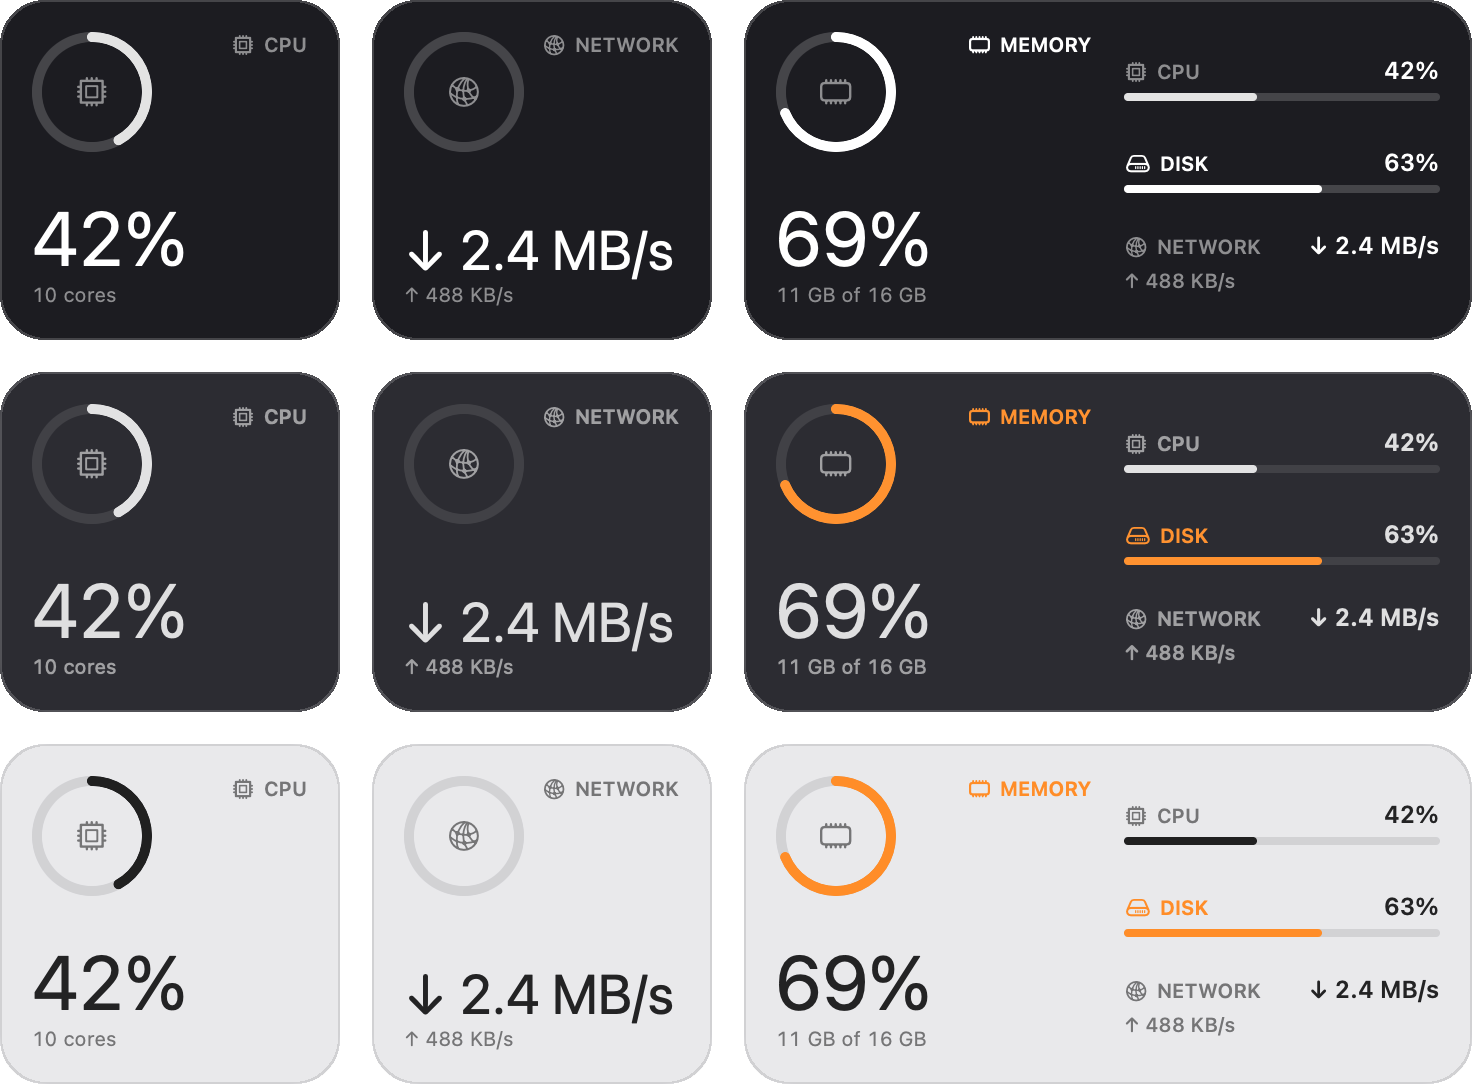
\includegraphics[width=\textwidth]{images/real-gallery.png}
\caption{\imagenreal{} · Widgets pequeños (CPU, red) y mediano
(memoria): cristal (arriba), oscuro y claro.}
\end{figure}

\begin{figure}[H]
\centering
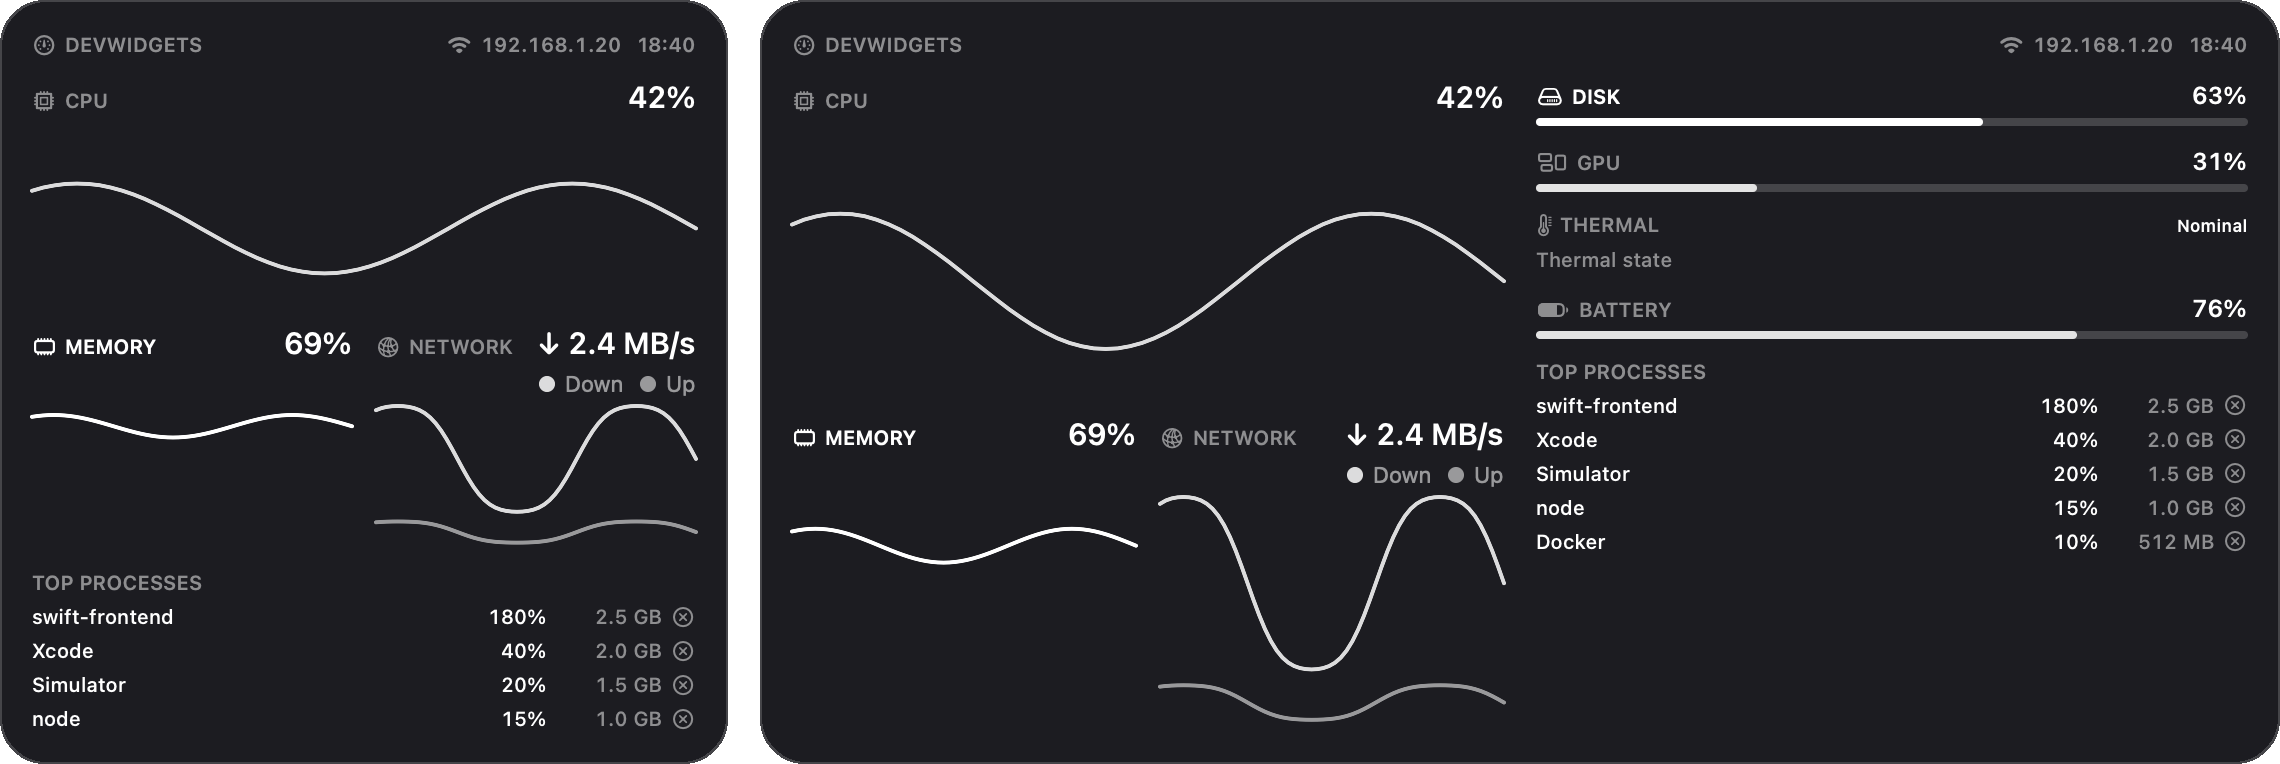
\includegraphics[width=\textwidth]{images/real-dashboards-clear.png}
\caption{\imagenreal{} · Widgets de panel grande y extra grande, en
cristal: histórico de CPU, memoria y red, discos, GPU, temperatura,
batería y procesos con botón de cerrar.}
\end{figure}

\begin{figure}[H]
\centering
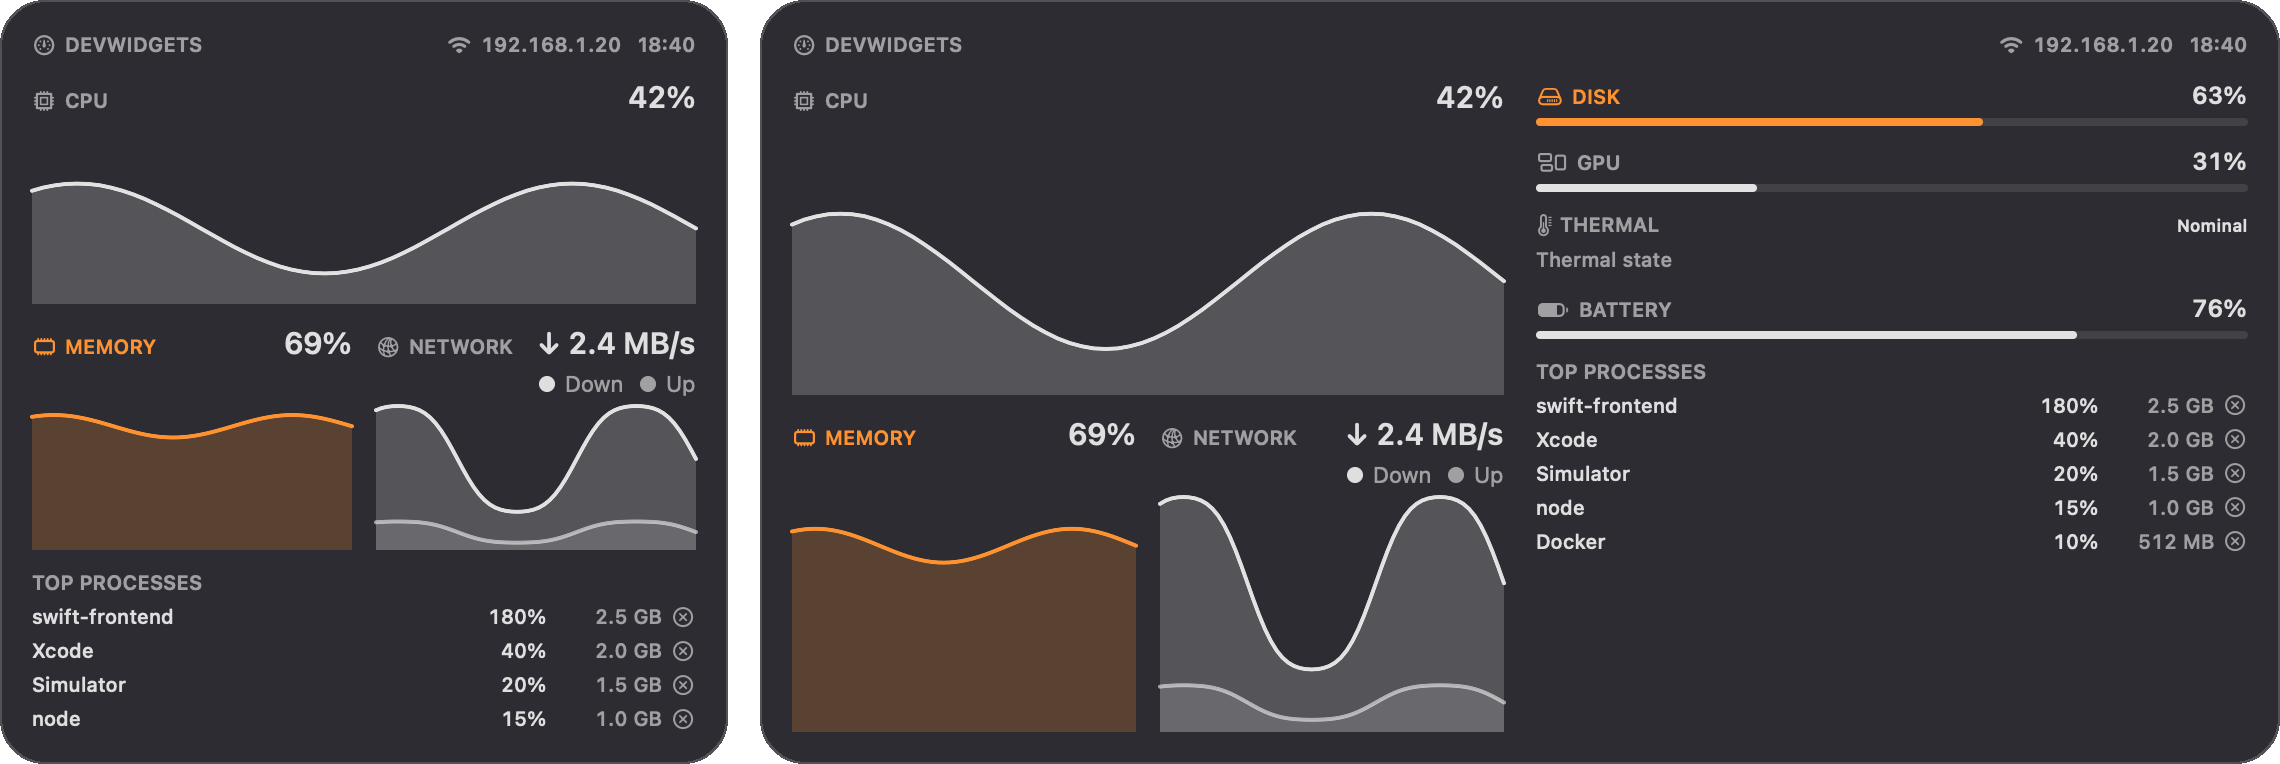
\includegraphics[width=\textwidth]{images/real-dashboards-dark.png}
\caption{\imagenreal{} · Widgets de panel, oscuro a todo color: el
naranja de memoria es el único color, porque su presión está
elevada.}
\end{figure}

\begin{figure}[H]
\centering
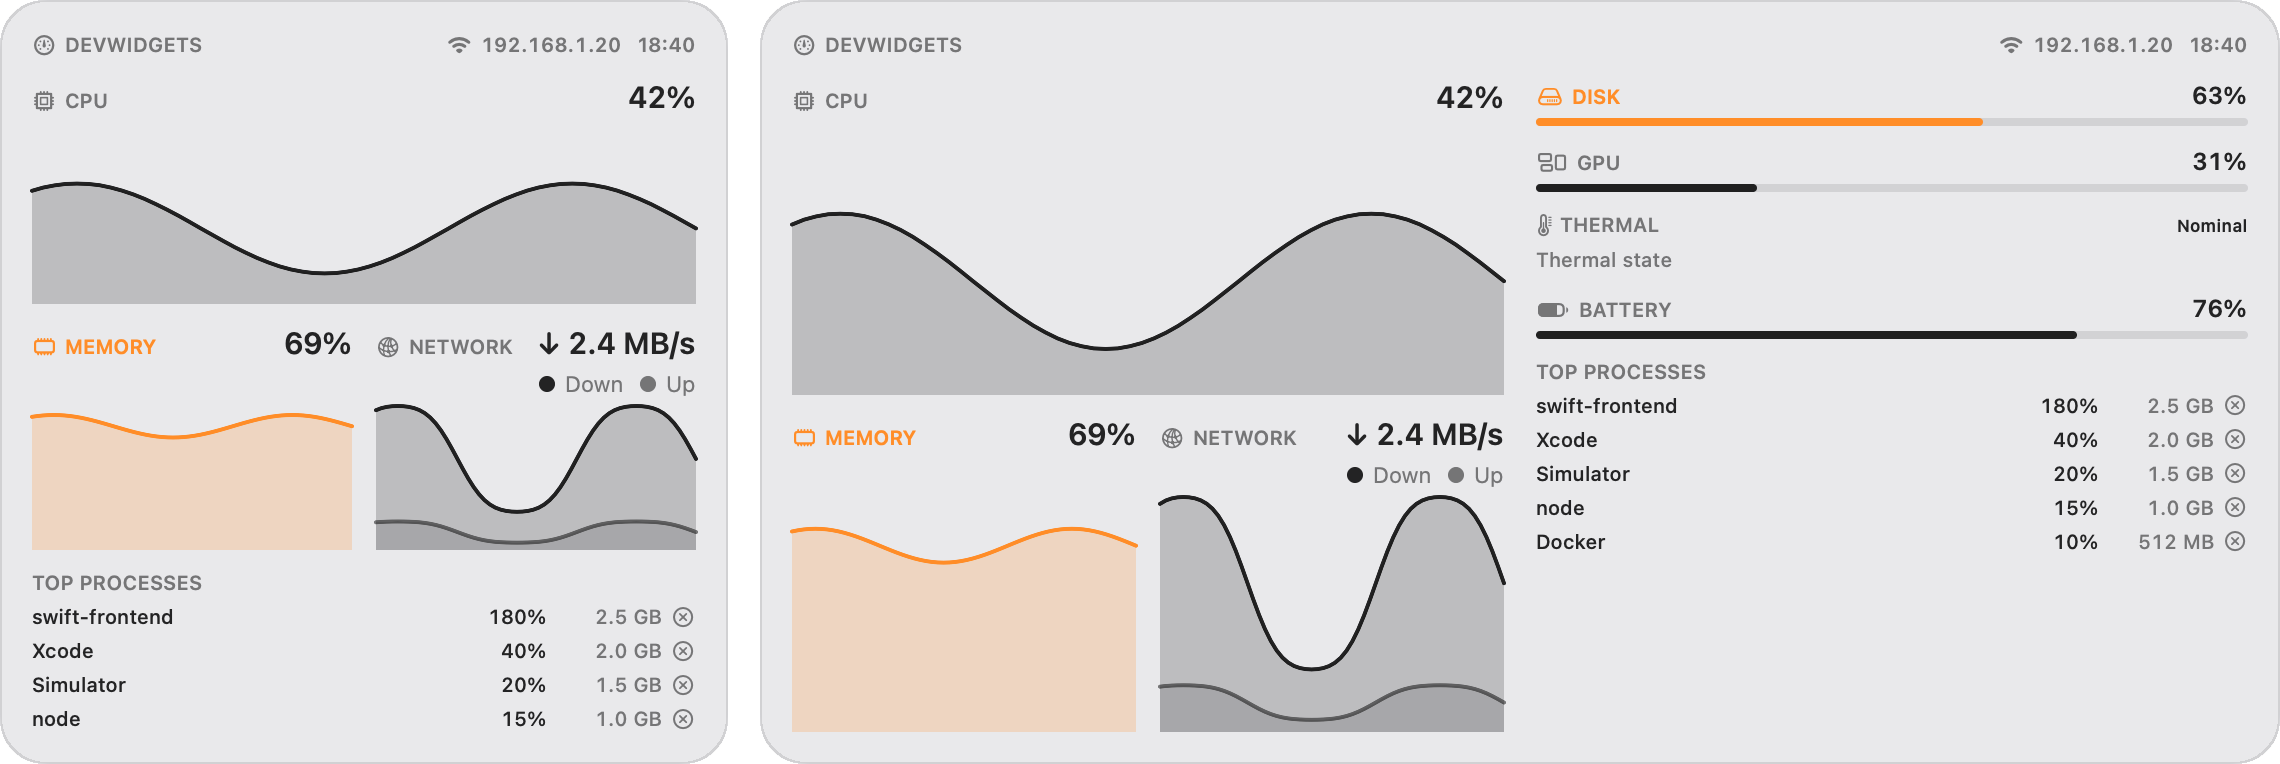
\includegraphics[width=\textwidth]{images/real-dashboards-light.png}
\caption{\imagenreal{} · Widgets de panel, claro a todo color.}
\end{figure}

\begin{figure}[H]
\centering
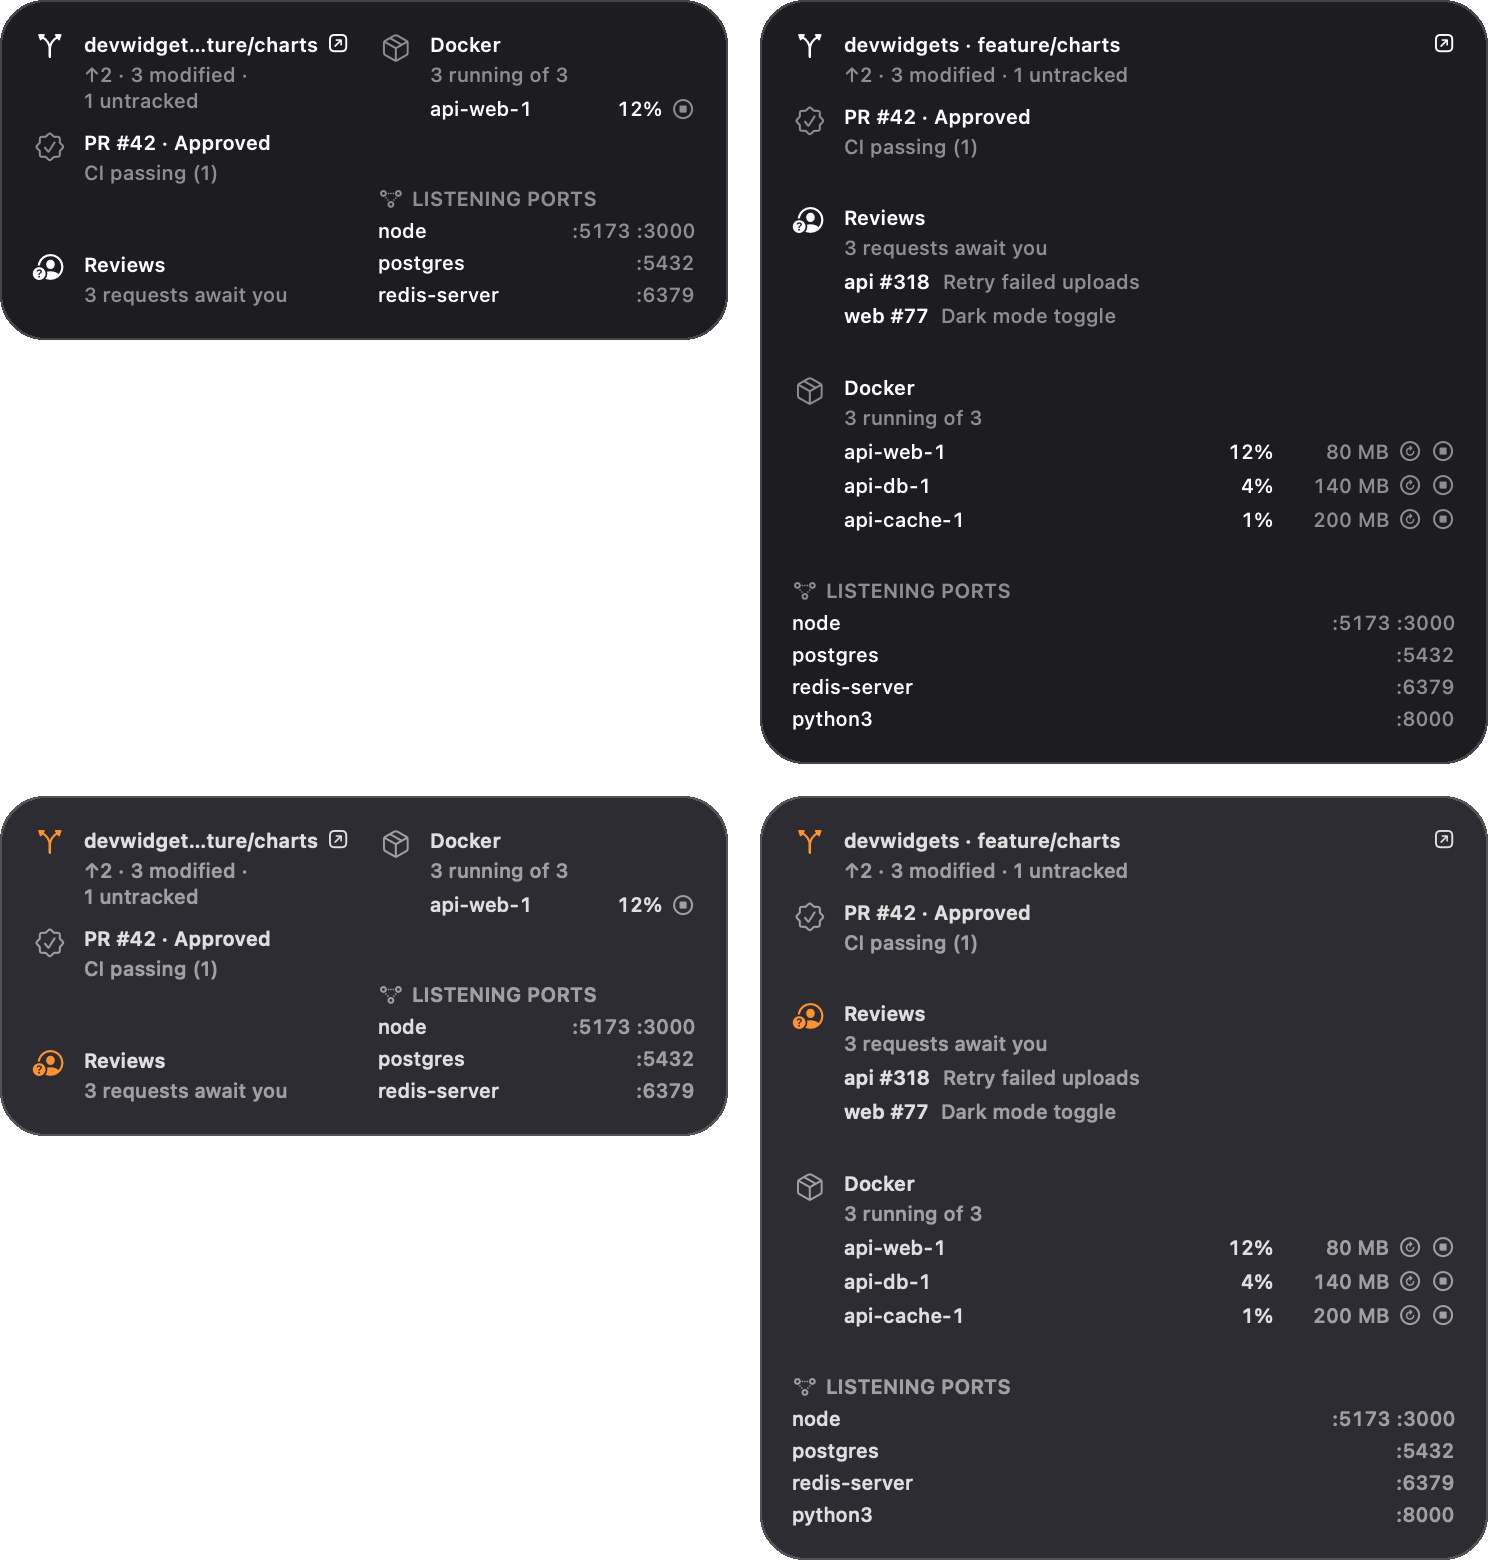
\includegraphics[width=0.9\textwidth]{images/real-context.png}
\caption{\imagenreal{} · Widget de contexto mediano y grande, cristal
y oscuro: Git, pull request y CI, revisiones pendientes, Docker con
botones de reiniciar y parar, y puertos.}
\end{figure}

\begin{figure}[H]
\centering
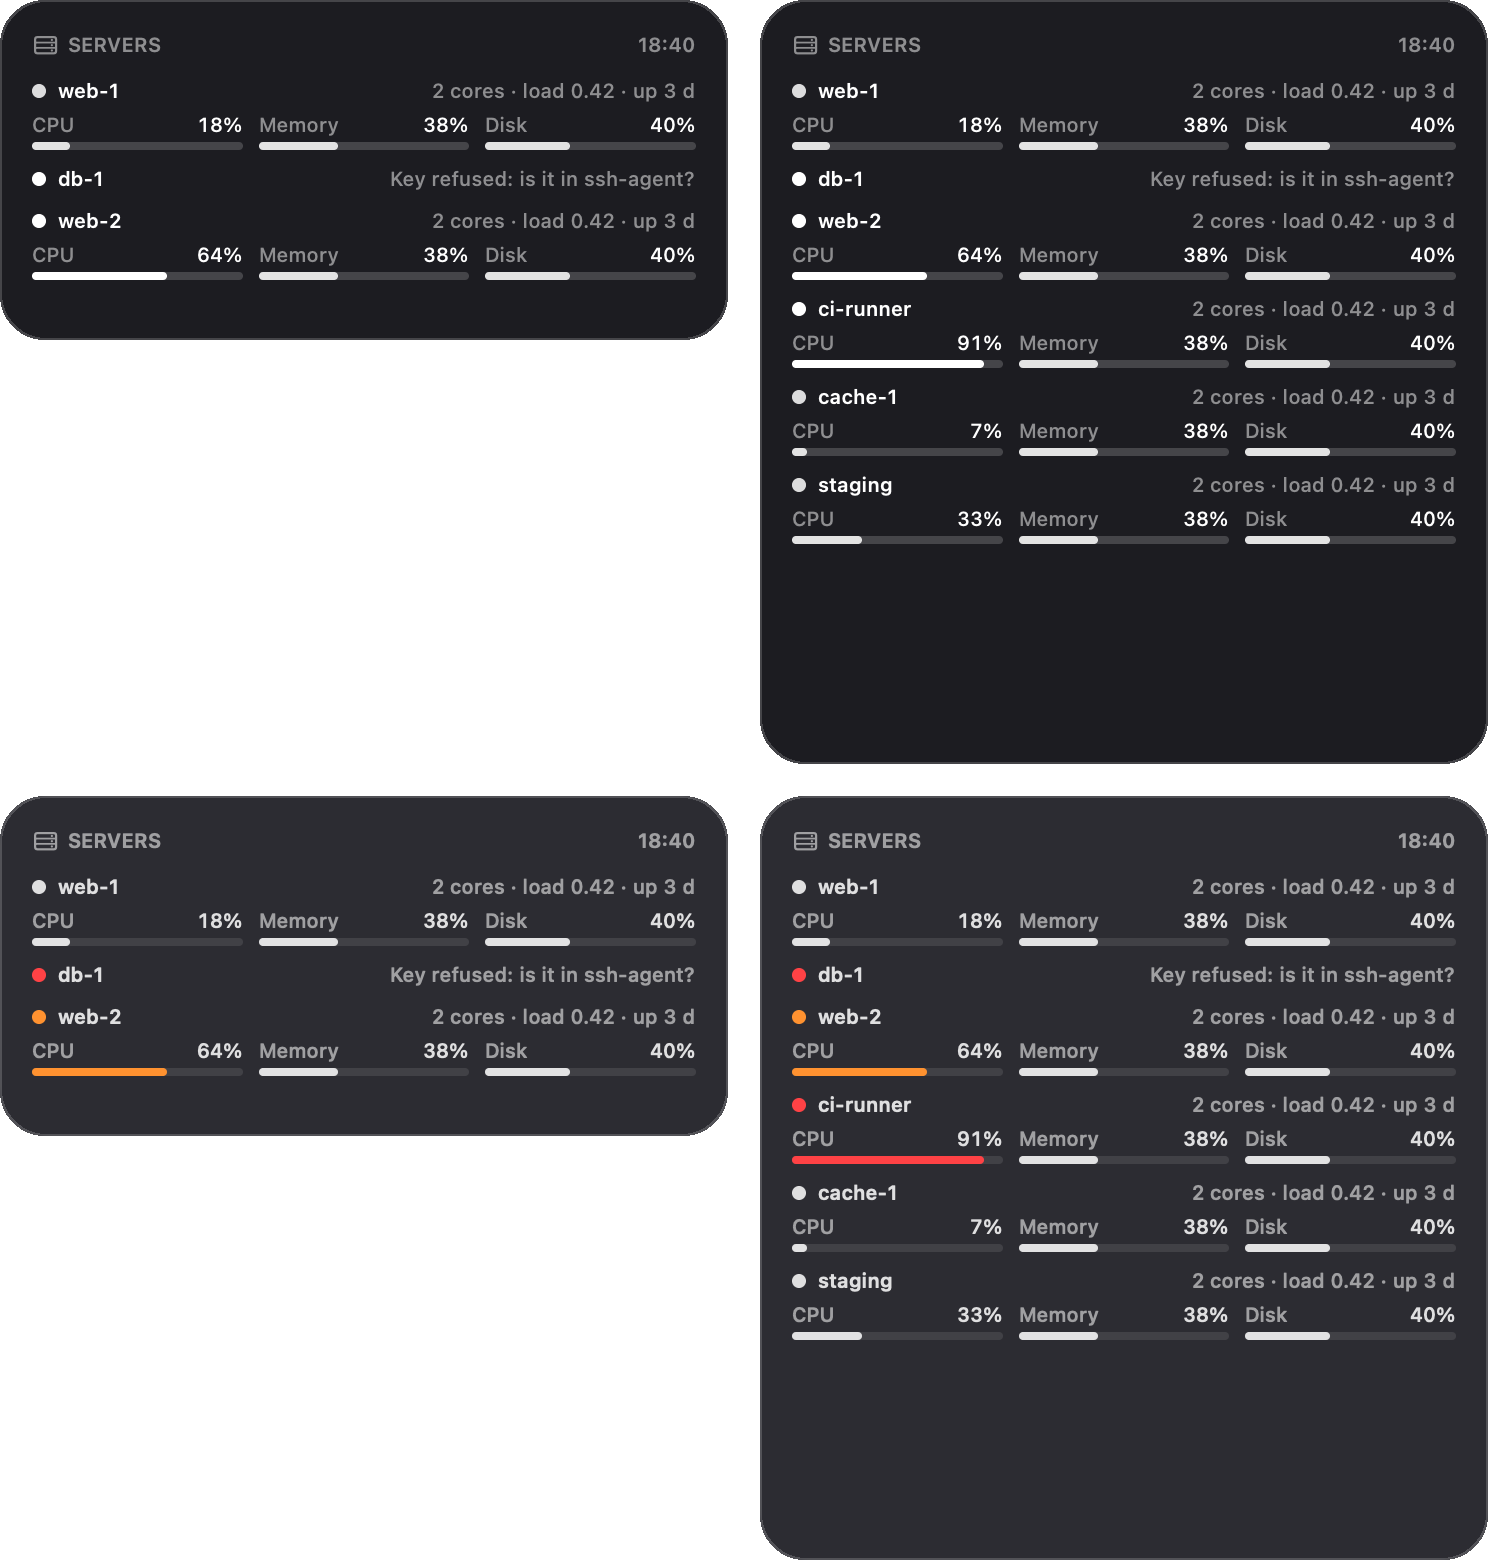
\includegraphics[width=0.9\textwidth]{images/real-servers.png}
\caption{\imagenreal{} · Widget de servidores mediano y grande, cristal
y oscuro. Seis servidores de ejemplo (\texttt{db-1} con la clave
rechazada).}
\end{figure}

\section{Cristal nativo y aprovechamiento del espacio}\label{sec:cristal}
\subsection{Explicación sencilla}
Marvin pidió que los widgets se vean \textbf{exactamente} como los
suyos del escritorio y que los medianos y grandes aprovechen mejor el
espacio. Antes cada widget pintaba su propio ``cristal'' (un degradado
blanco sobre un material translúcido) y usaba verde, naranja y rojo
por todas partes. Eso no es el cristal de macOS: es una imitación que
se nota. Ahora el widget no pinta fondo propio, deja que macOS ponga su
Liquid Glass, el texto es blanco y gris como en sus widgets, las cifras
son grandes y el color solo aparece cuando algo necesita atención.

\begin{figure}[H]
\centering
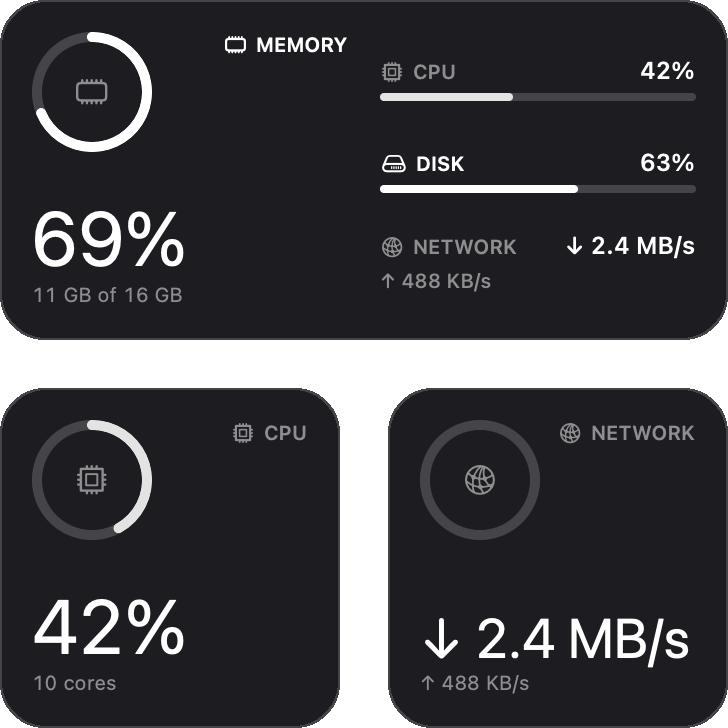
\includegraphics[width=\textwidth]{images/comparison-reference.png}
\caption{\imagenreal{} · DevWidgets en la misma disposición que los
widgets nativos de Marvin en su escritorio (memoria mediano, CPU y red
pequeños), con los que se comparó. Solo los widgets, sin fondo; la
captura de su escritorio no se incluye.}
\end{figure}

\subsection{Explicación técnica}
\paragraph{Qué dice Apple.} En macOS~26, con los widgets en cristal o
tintados, el sistema dibuja el widget en modo \texttt{accented}: quita
todo lo que esté en \texttt{containerBackground}, pone su Liquid Glass
y tiñe el contenido (blanco en cristal) conservando la opacidad.
Recomienda leer \texttt{widgetRenderingMode}, dejar los degradados y
rellenos para el modo a todo color y no imitar el cristal.

\paragraph{Cambios en el cristal.}
\begin{itemize}
  \item Fuera \texttt{WidgetGlassBackground} (degradado +
    \texttt{.ultraThinMaterial}). Los cuatro widgets usan
    \texttt{systemWidgetBackground()}, que es
    \texttt{.containerBackground(.fill.tertiary, for: .widget)}, el
    fondo de la plantilla de Xcode. En cristal el sistema lo quita.
  \item Color solo por estado: \texttt{LoadLevel.tint} es
    \texttt{.primary} cuando todo va bien, naranja si está elevado y
    rojo si es crítico. Iconos y títulos en \texttt{.secondary} salvo
    con aviso.
  \item Las gráficas leen \texttt{widgetRenderingMode}: el relleno
    translúcido bajo la línea solo se dibuja a todo color. La segunda
    serie (subida) es \texttt{.secondary} en vez de azul.
  \item Jerarquía como la del sistema: etiquetas pequeñas en mayúsculas
    (\texttt{CPU}, \texttt{TOP PROCESSES}, como ``TUESDAY'' en el
    calendario), cifras grandes (38\,pt, peso normal, como el ``85\,\%''
    de la batería) y anillo fino (5\,pt) con el símbolo dentro.
\end{itemize}

\paragraph{Cambios en el espacio.} Márgenes del sistema (16\,pt, los de
WidgetKit, sin añadir más).
\begin{itemize}
  \item \textbf{Pequeño}: anillo arriba a la izquierda, título arriba a
    la derecha, cifra grande y detalle abajo, como el widget de
    batería.
  \item \textbf{Métrica mediano}: la mitad izquierda es el pequeño; las
    tres filas de la derecha se reparten toda la altura.
  \item \textbf{Panel grande}: cuatro procesos en vez de tres.
  \item \textbf{Contexto}: el mediano añade la fila de revisiones y una
    tercera línea de puertos; el grande reparte Git, revisiones, Docker
    y puertos en toda la altura, como la agenda del calendario.
  \item \textbf{Servidores mediano}: hasta tres servidores, los que
    quepan (\texttt{ViewThatFits}); antes, dos y un hueco vacío.
  \item Datos de ejemplo más realistas para la galería: tres
    contenedores, cinco puertos, dos revisiones, cinco procesos y seis
    servidores.
\end{itemize}

\begin{figure}[H]
\centering
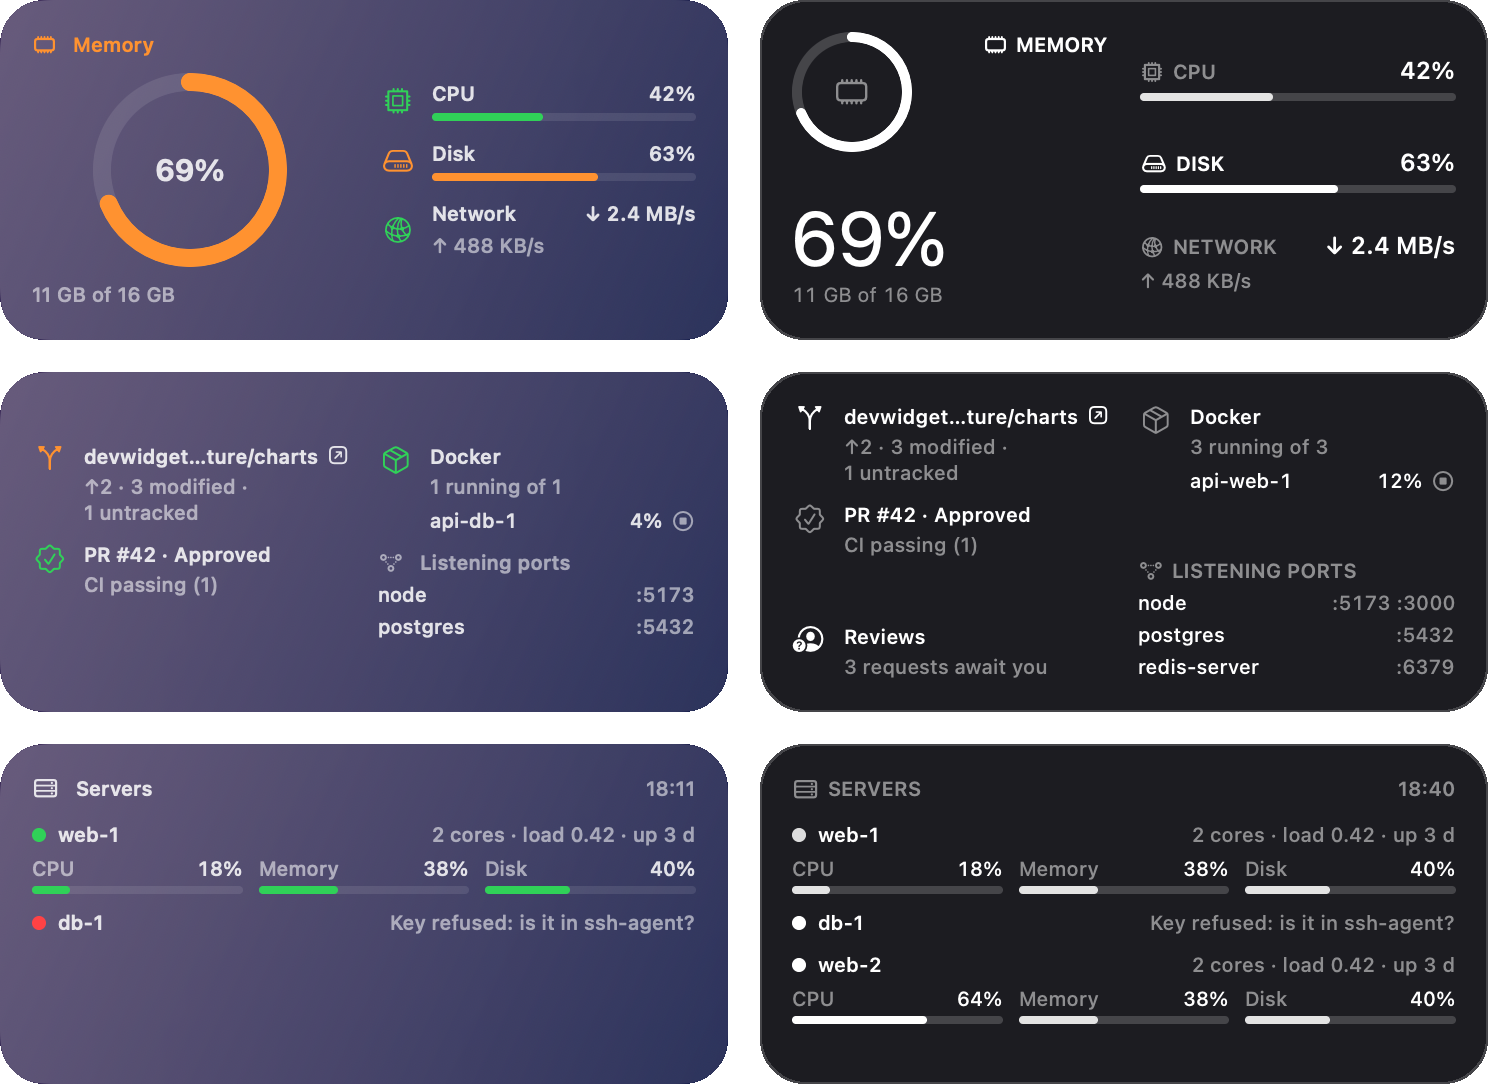
\includegraphics[width=0.95\textwidth]{images/before-after-medium.png}
\caption{\imagenreal{} · Medianos antes (oscuro, cristal imitado) y
después (presentación en cristal, sobre placa neutra).}
\end{figure}

\begin{figure}[H]
\centering
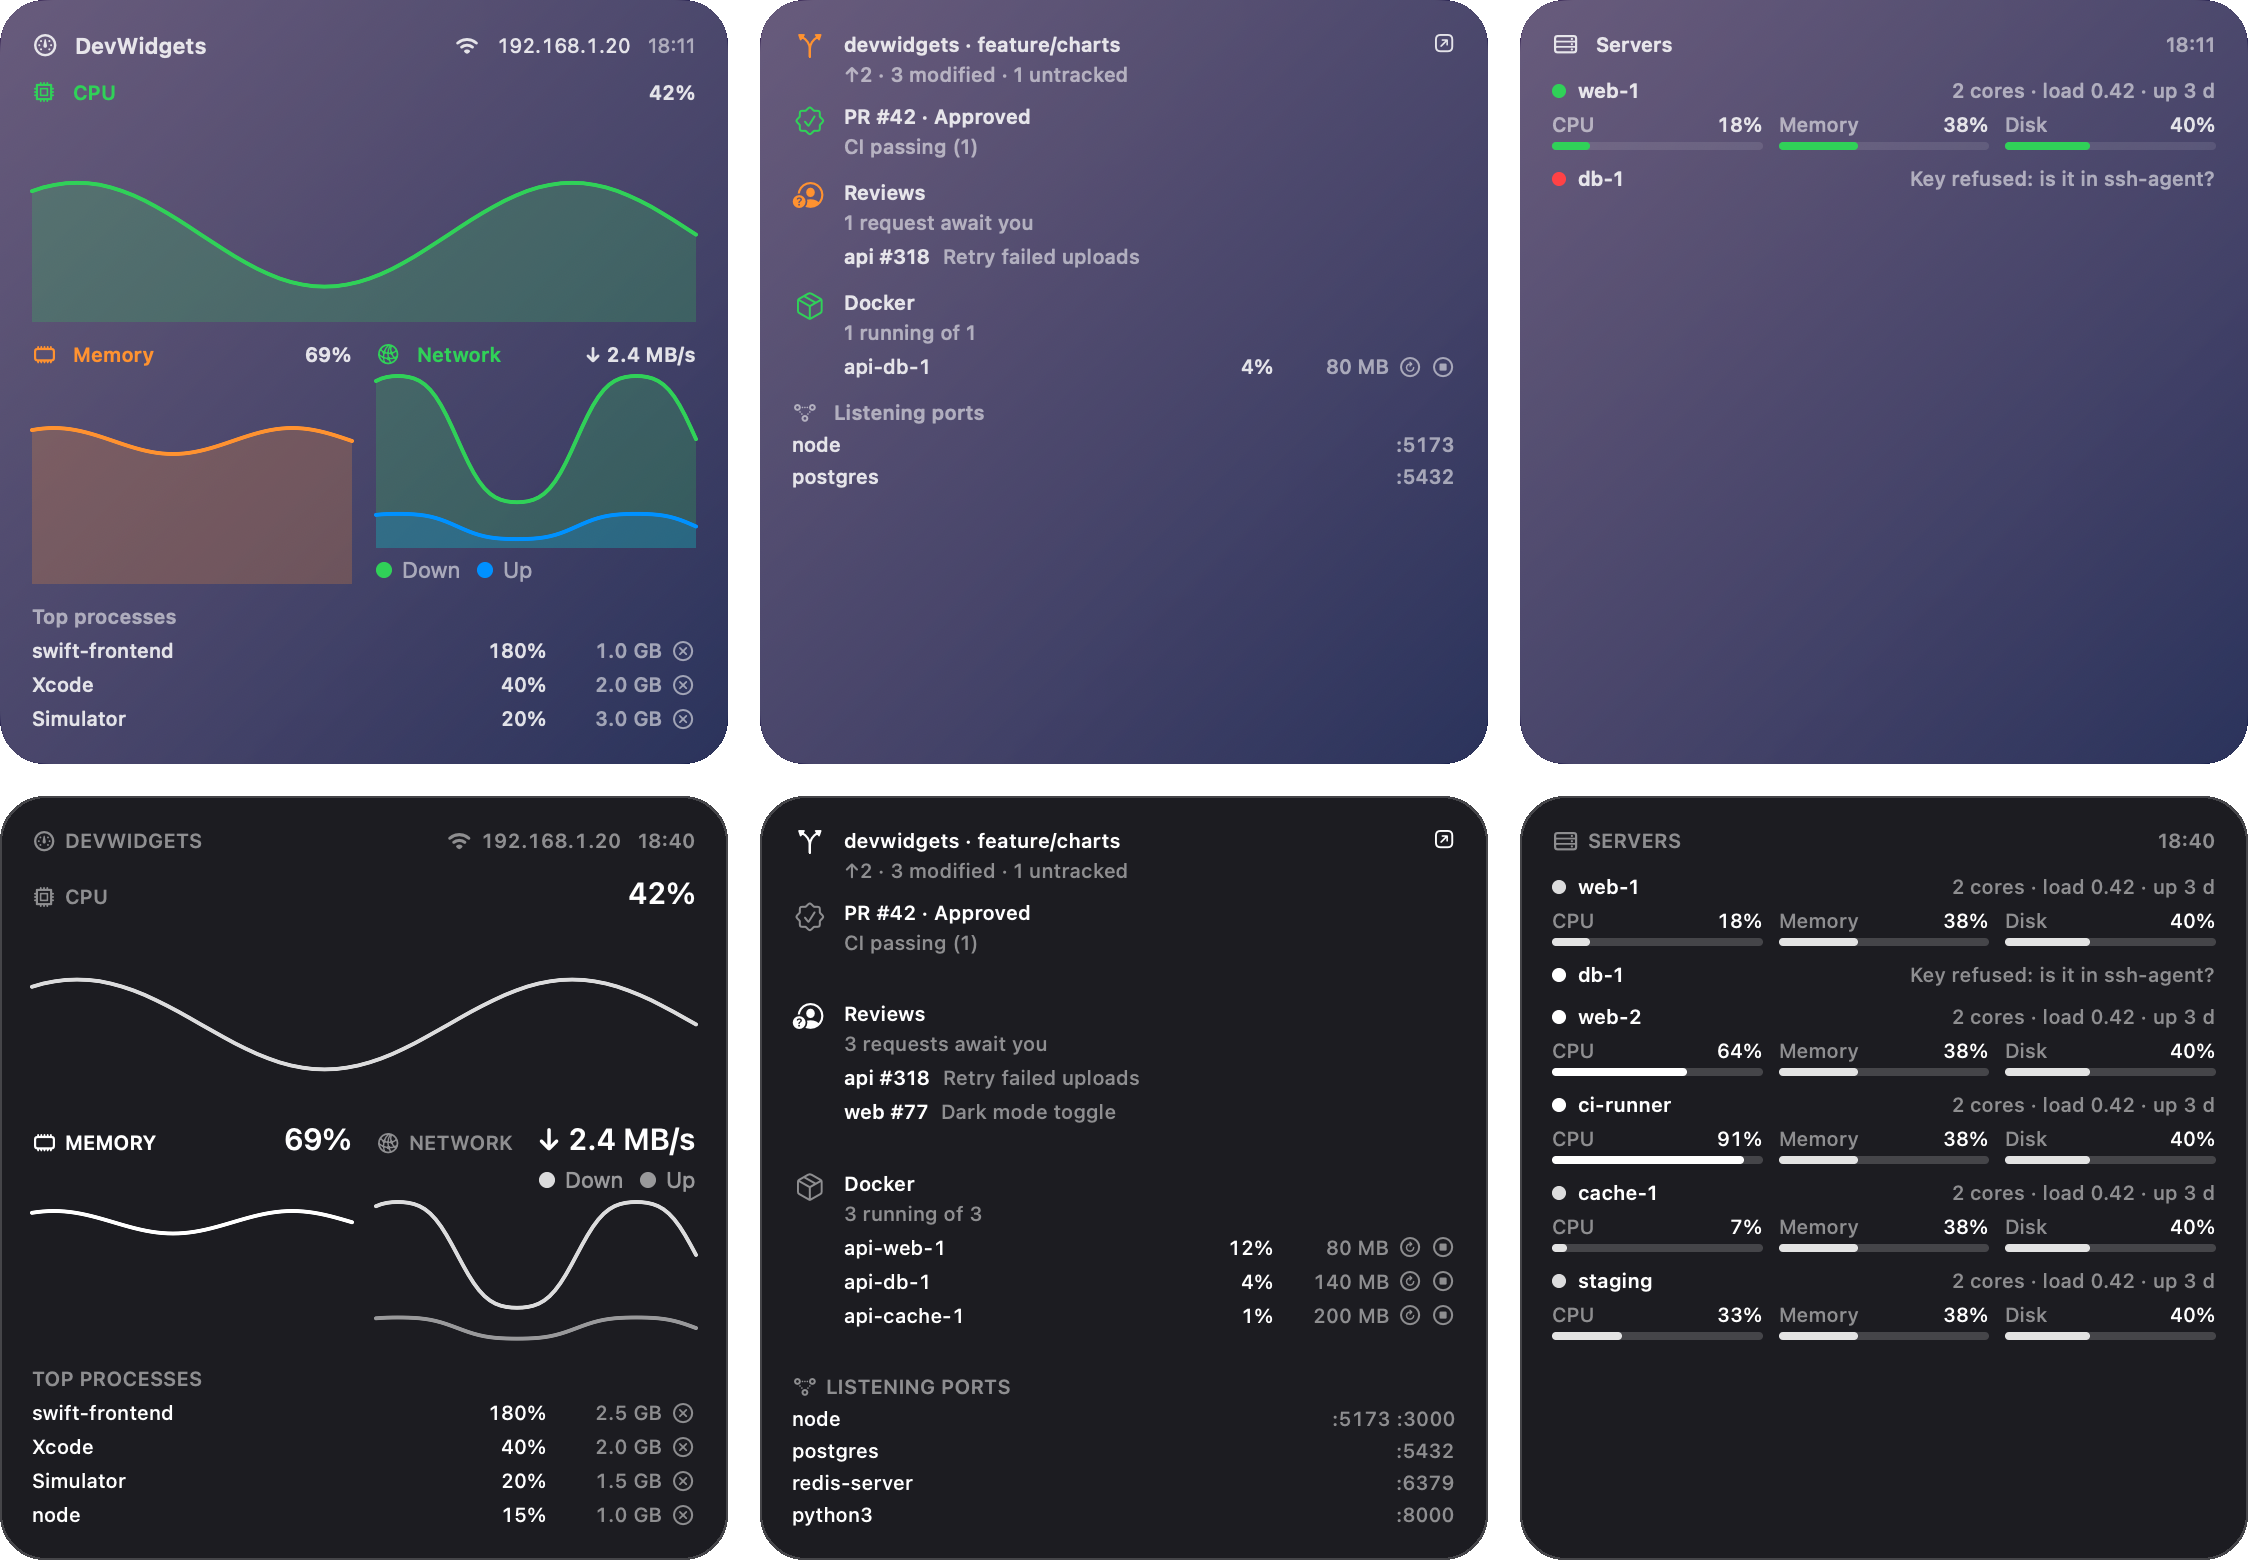
\includegraphics[width=\textwidth]{images/before-after-large.png}
\caption{\imagenreal{} · Grandes antes (arriba) y después (abajo).}
\end{figure}

\paragraph{Autocrítica.}
\begin{itemize}
  \item Las imágenes no son capturas del escritorio: el contenido es
    real, el fondo de cristal es una placa neutra.
  \item Con \texttt{.primary} cuando todo va bien, en cristal un aviso
    se distingue solo por el blanco más intenso del título (el sistema
    quita el color); en la app y a todo color sigue siendo naranja o
    rojo.
  \item El nombre del proyecto se corta en el contexto mediano cuando
    la rama es larga.
  \item Falta comprobar en el escritorio real que \texttt{.fill.tertiary}
    a todo color se ve como los widgets de Apple; si no, la alternativa
    es otro estilo del sistema, nunca un fondo propio.
\end{itemize}

\section{Capturas reales de Linux}\label{sec:capturas}
Las imágenes de esta sección llevan la etiqueta \capturareal{}: la app
\texttt{devwidgets} instalada desde el \texttt{.deb}, funcionando en
la máquina de pruebas (escritorio XFCE virtual, sin GPU) y capturada
con \texttt{xwd}. Los datos son de esa máquina: los procesos
\texttt{yes} son la carga de prueba, \texttt{devwidgets-test} es el
\texttt{sshd} local y \texttt{devwidgets-closed} un puerto cerrado.
Docker aparece como ``Not installed'' y GitHub sin remoto porque así
es en la máquina. Solo se han recortado los bordes.

\begin{figure}[H]
\centering
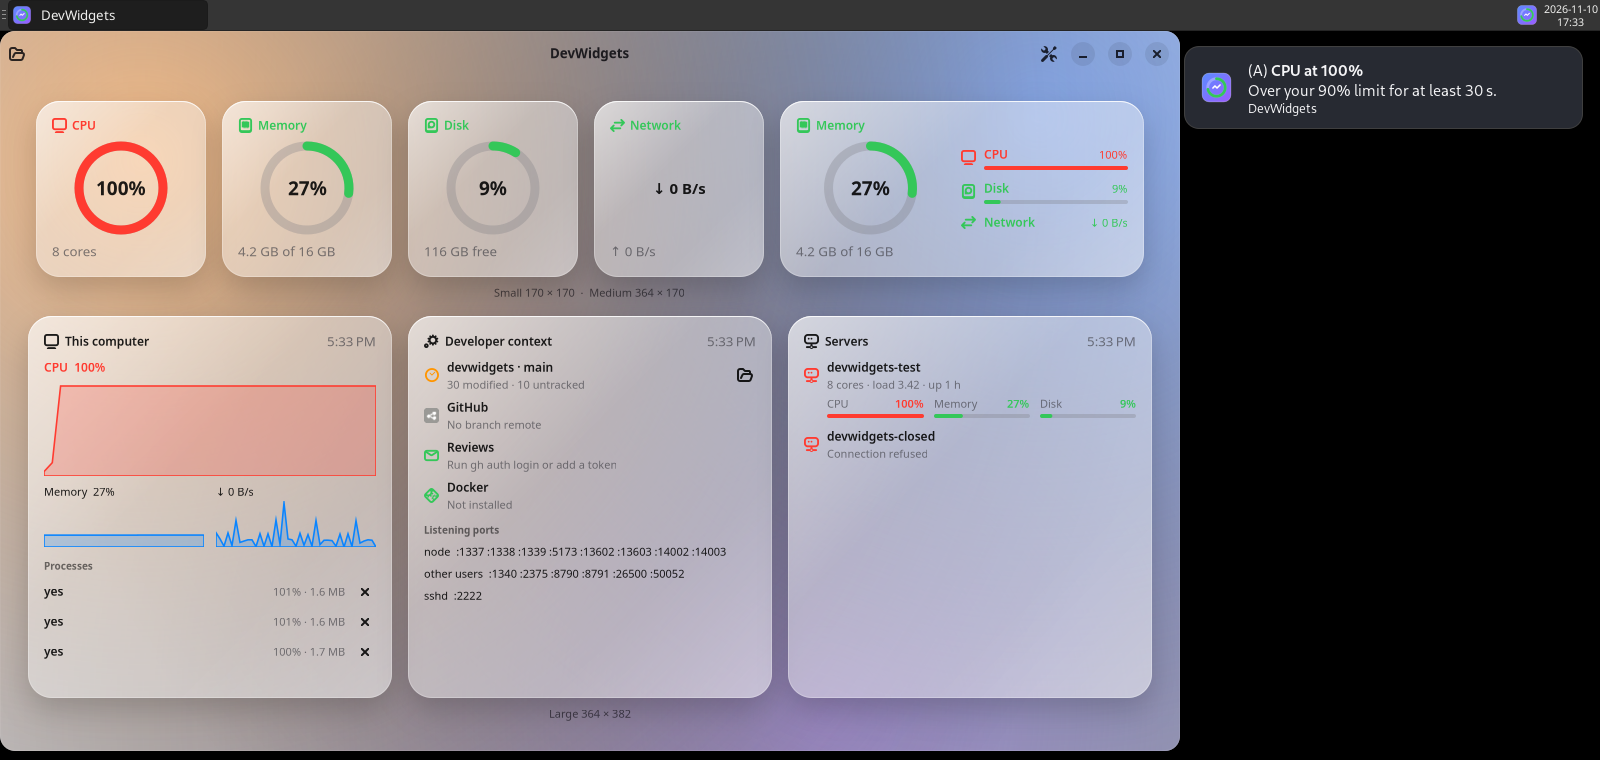
\includegraphics[width=\textwidth]{images/linux-dashboard-light.png}
\caption{\capturareal{} · Panel en modo claro: fila de tarjetas
pequeñas y mediana, y las grandes de este equipo, contexto y
servidores, con sus tamaños de macOS rotulados. CPU al 100\,\% por la
carga de prueba y su notificación real (\texttt{dunst}). Arriba a la
derecha, el icono en la bandeja.}
\end{figure}

\begin{figure}[H]
\centering
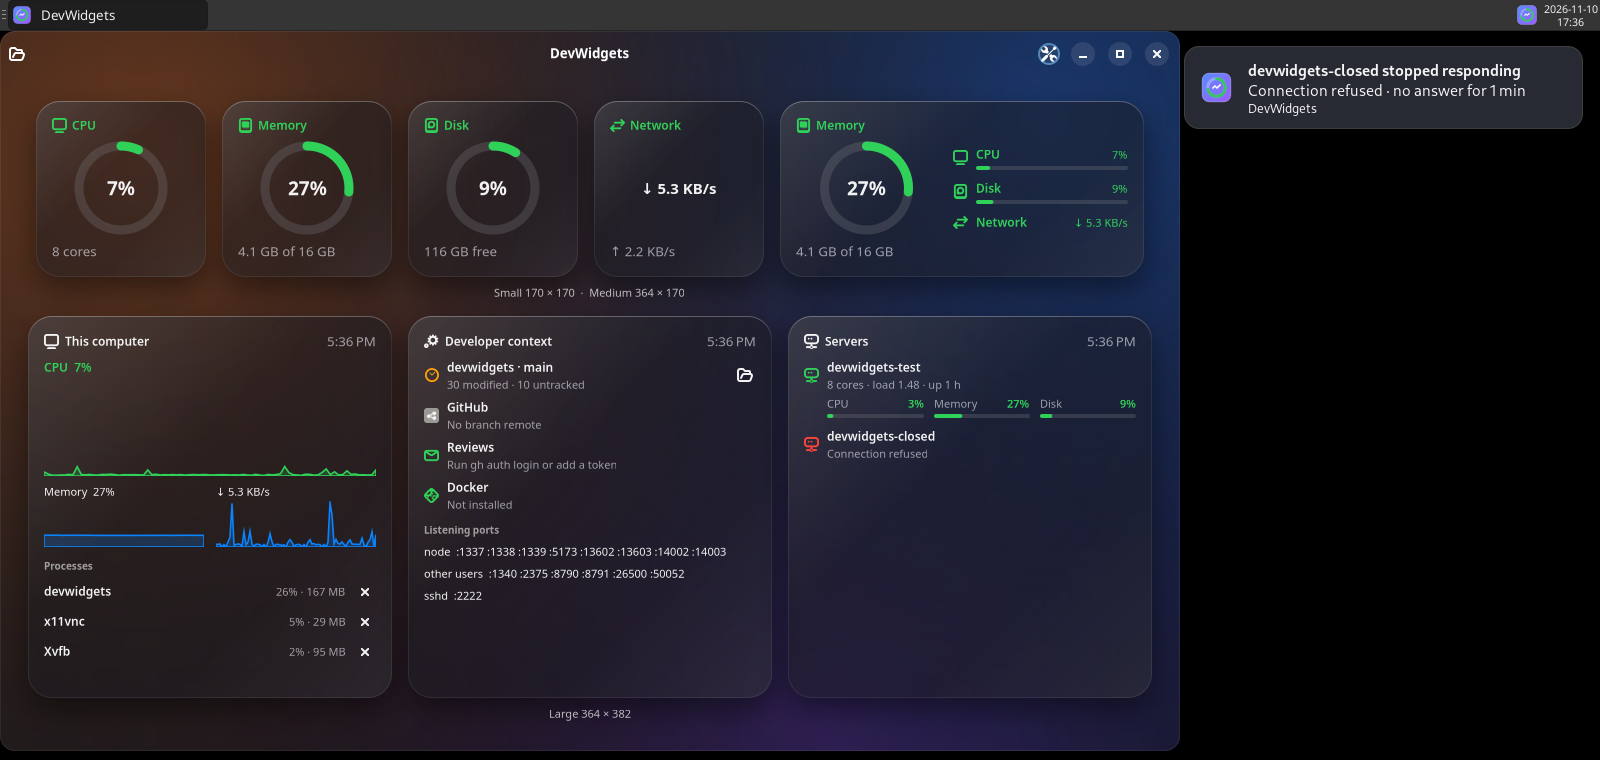
\includegraphics[width=\textwidth]{images/linux-dashboard-dark.png}
\caption{\capturareal{} · Modo oscuro y aviso nuevo de servidor que
deja de responder (\texttt{devwidgets-closed}, tras 1\,min).}
\end{figure}

\begin{figure}[H]
\centering
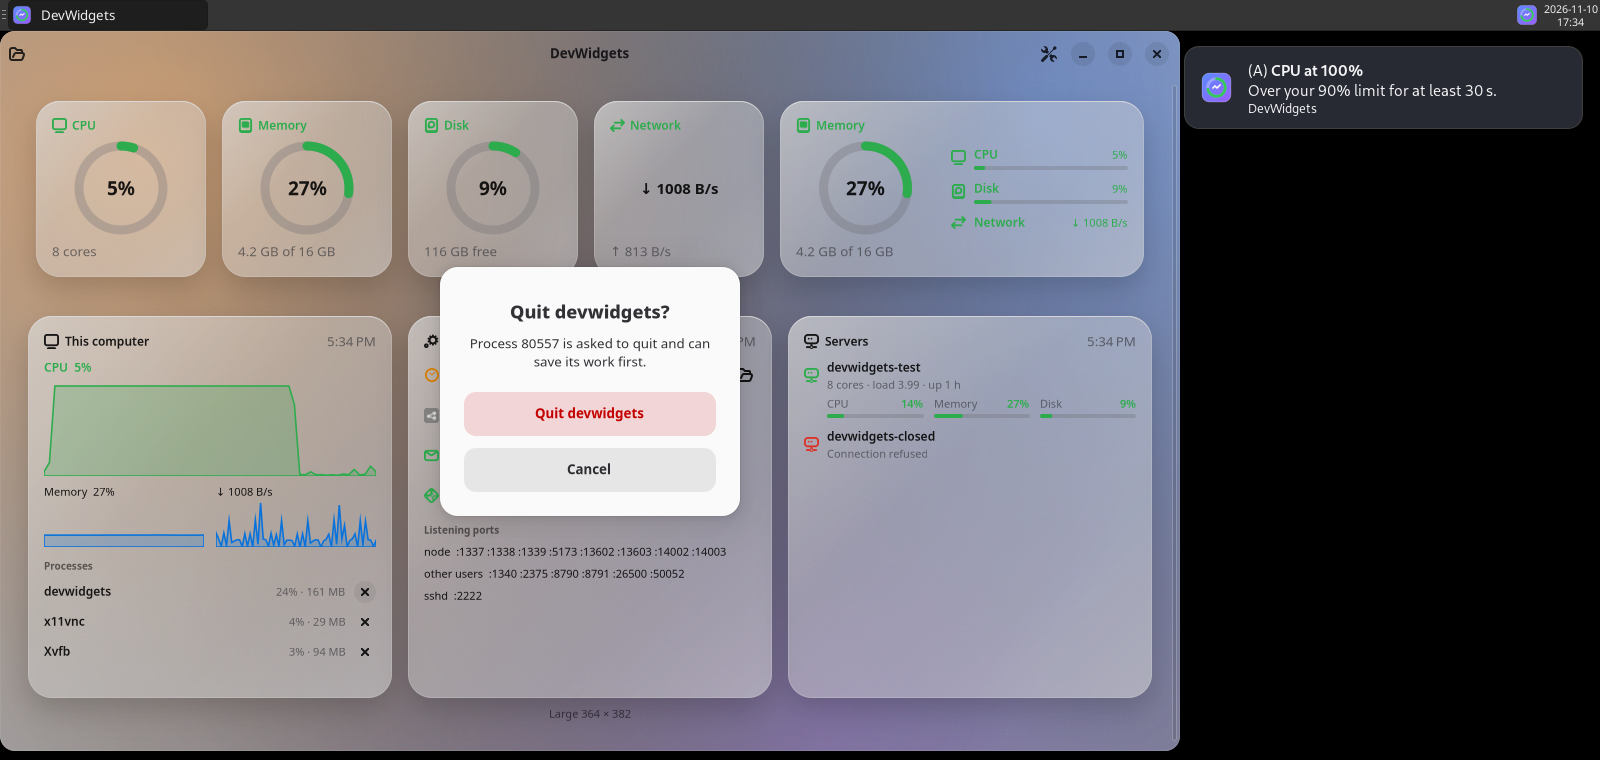
\includegraphics[width=0.49\textwidth]{images/linux-confirm.png}
\hfill
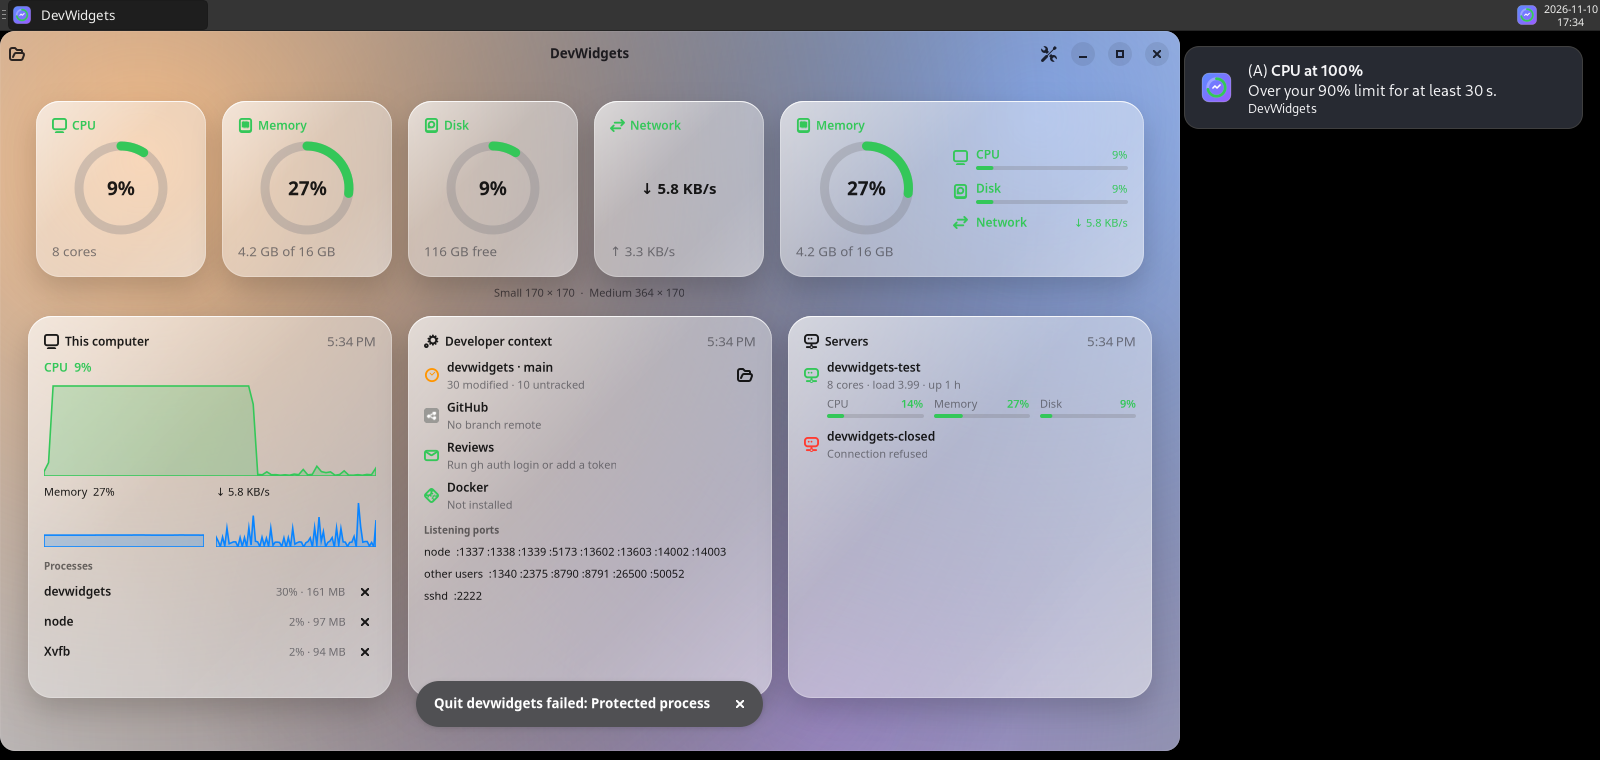
\includegraphics[width=0.49\textwidth]{images/linux-toast.png}
\caption{\capturareal{} · Confirmación al cerrar un proceso (como en
macOS) y, tras confirmar con un proceso protegido, el aviso de
error.}
\end{figure}

\begin{figure}[H]
\centering
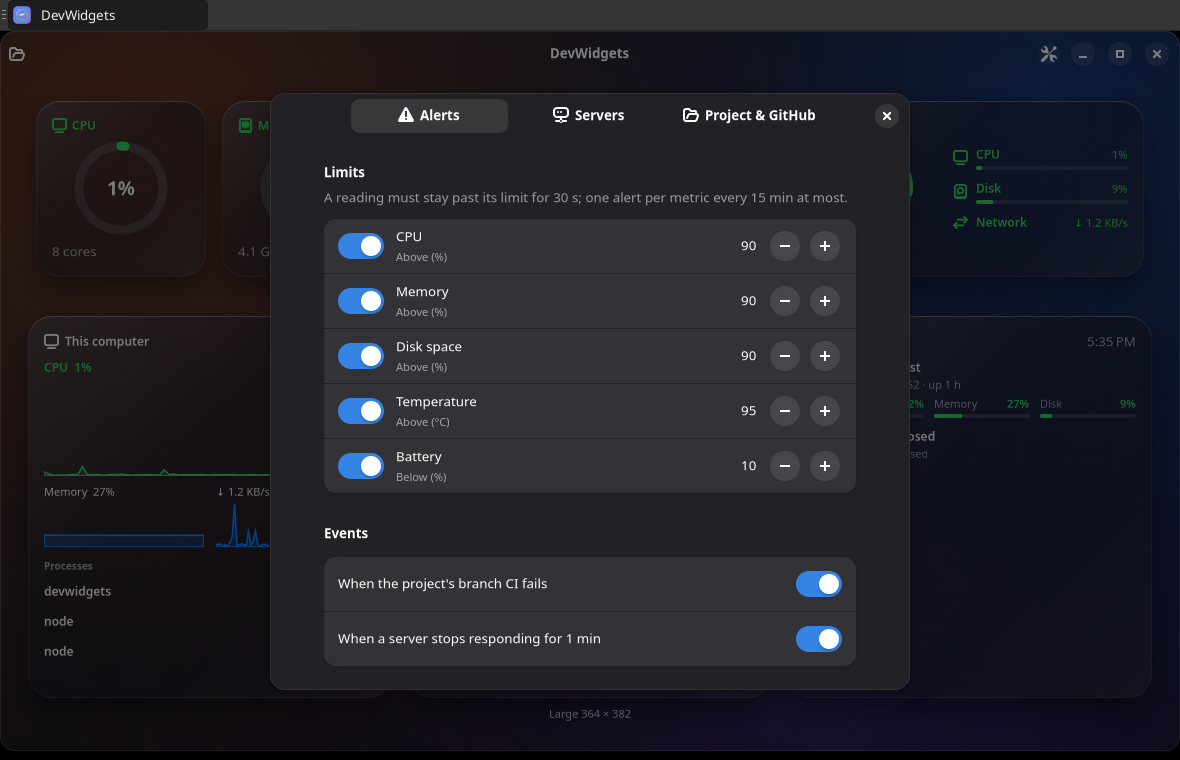
\includegraphics[width=0.49\textwidth]{images/linux-preferences-alerts.png}
\hfill
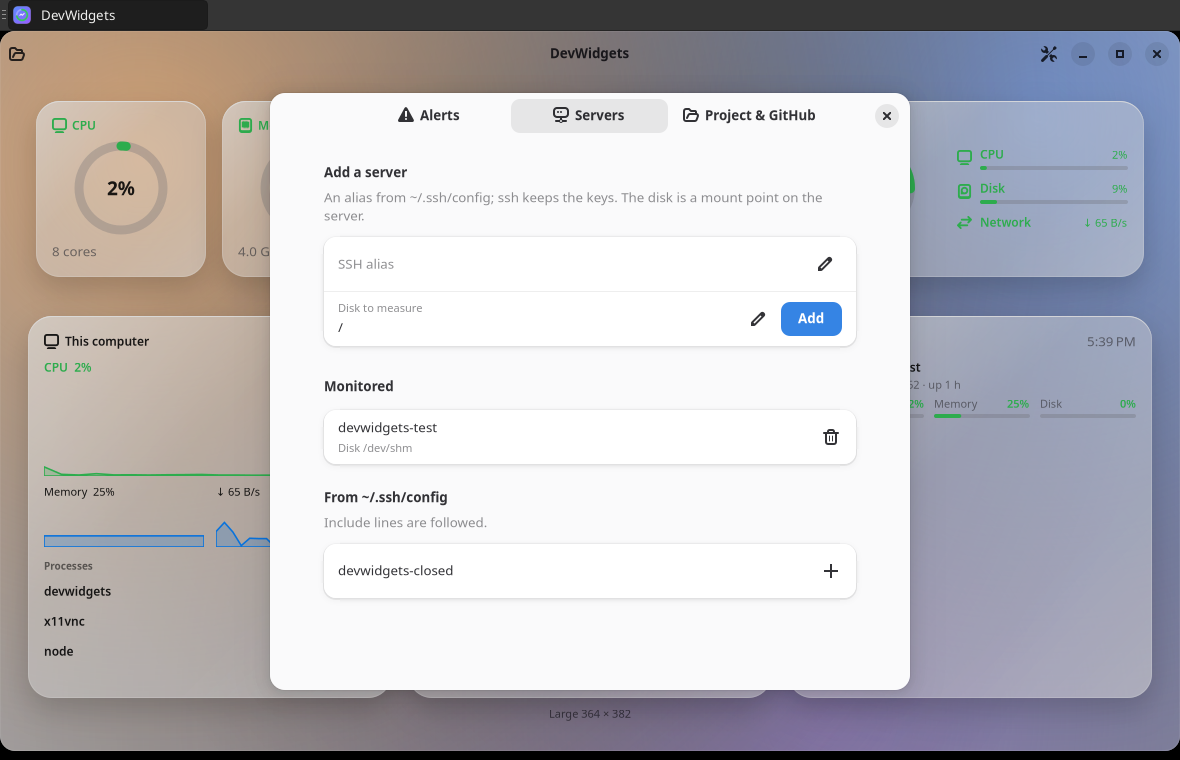
\includegraphics[width=0.49\textwidth]{images/linux-preferences-servers.png}
\caption{\capturareal{} · Ajustes: alertas (modo oscuro) y servidores,
con \texttt{devwidgets-test} midiendo el disco \texttt{/dev/shm} y
\texttt{devwidgets-closed} sugerido desde un fichero incluido con
\texttt{Include}.}
\end{figure}

\begin{figure}[H]
\centering
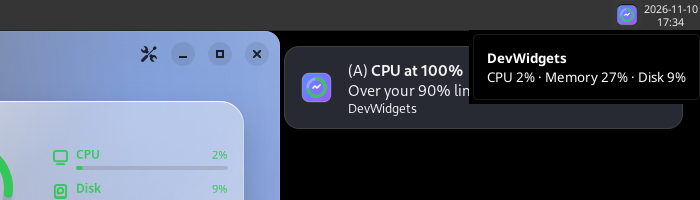
\includegraphics[width=0.6\textwidth]{images/linux-tray-tooltip.png}
\caption{\capturareal{} · Resumen del icono de la bandeja.}
\end{figure}

\section{Maquetas que quedan}
Las maquetas de los widgets en modo claro, oscuro y cristal se han
sustituido por imágenes reales (sección~\ref{sec:imagenes}). Quedan como
\maqueta{}s HTML/CSS, renderizadas con Chromium sin interfaz, el modo
tintado y las ventanas de la app (panel de la barra de menús, Ajustes,
avisos y diálogos), que solo se pueden capturar con la app instalada.
Reproducen la disposición de las vistas SwiftUI, pero \textbf{no son
capturas de macOS}. En las
de la fase 2, GPU, batería y temperatura son \textbf{valores de
ejemplo}. El cristal se imita
con desenfoque y brillos; el Liquid Glass real refracta el fondo y
reacciona a la luz.

\begin{figure}[H]
\centering
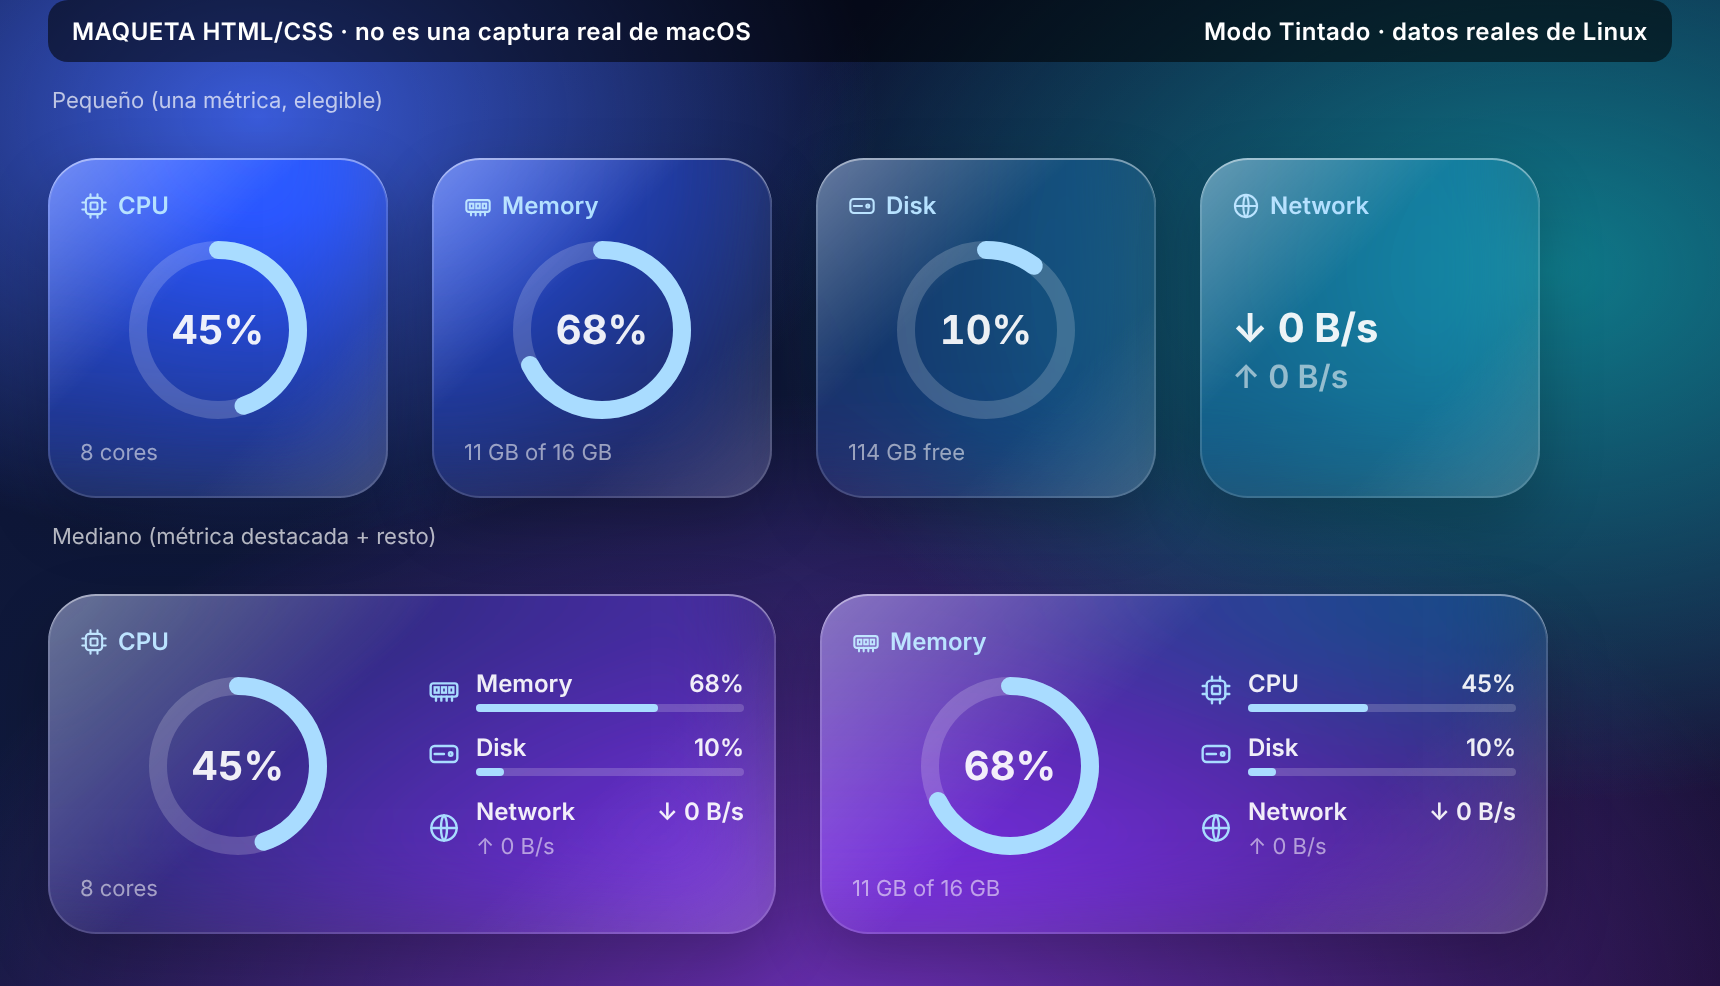
\includegraphics[width=\textwidth]{images/mockup-gallery-tinted.png}
\caption{\maqueta{} · Modo tintado: el sistema tiñe con un único
color los elementos marcados con \texttt{widgetAccentable()}.}
\end{figure}

\begin{figure}[H]
\centering
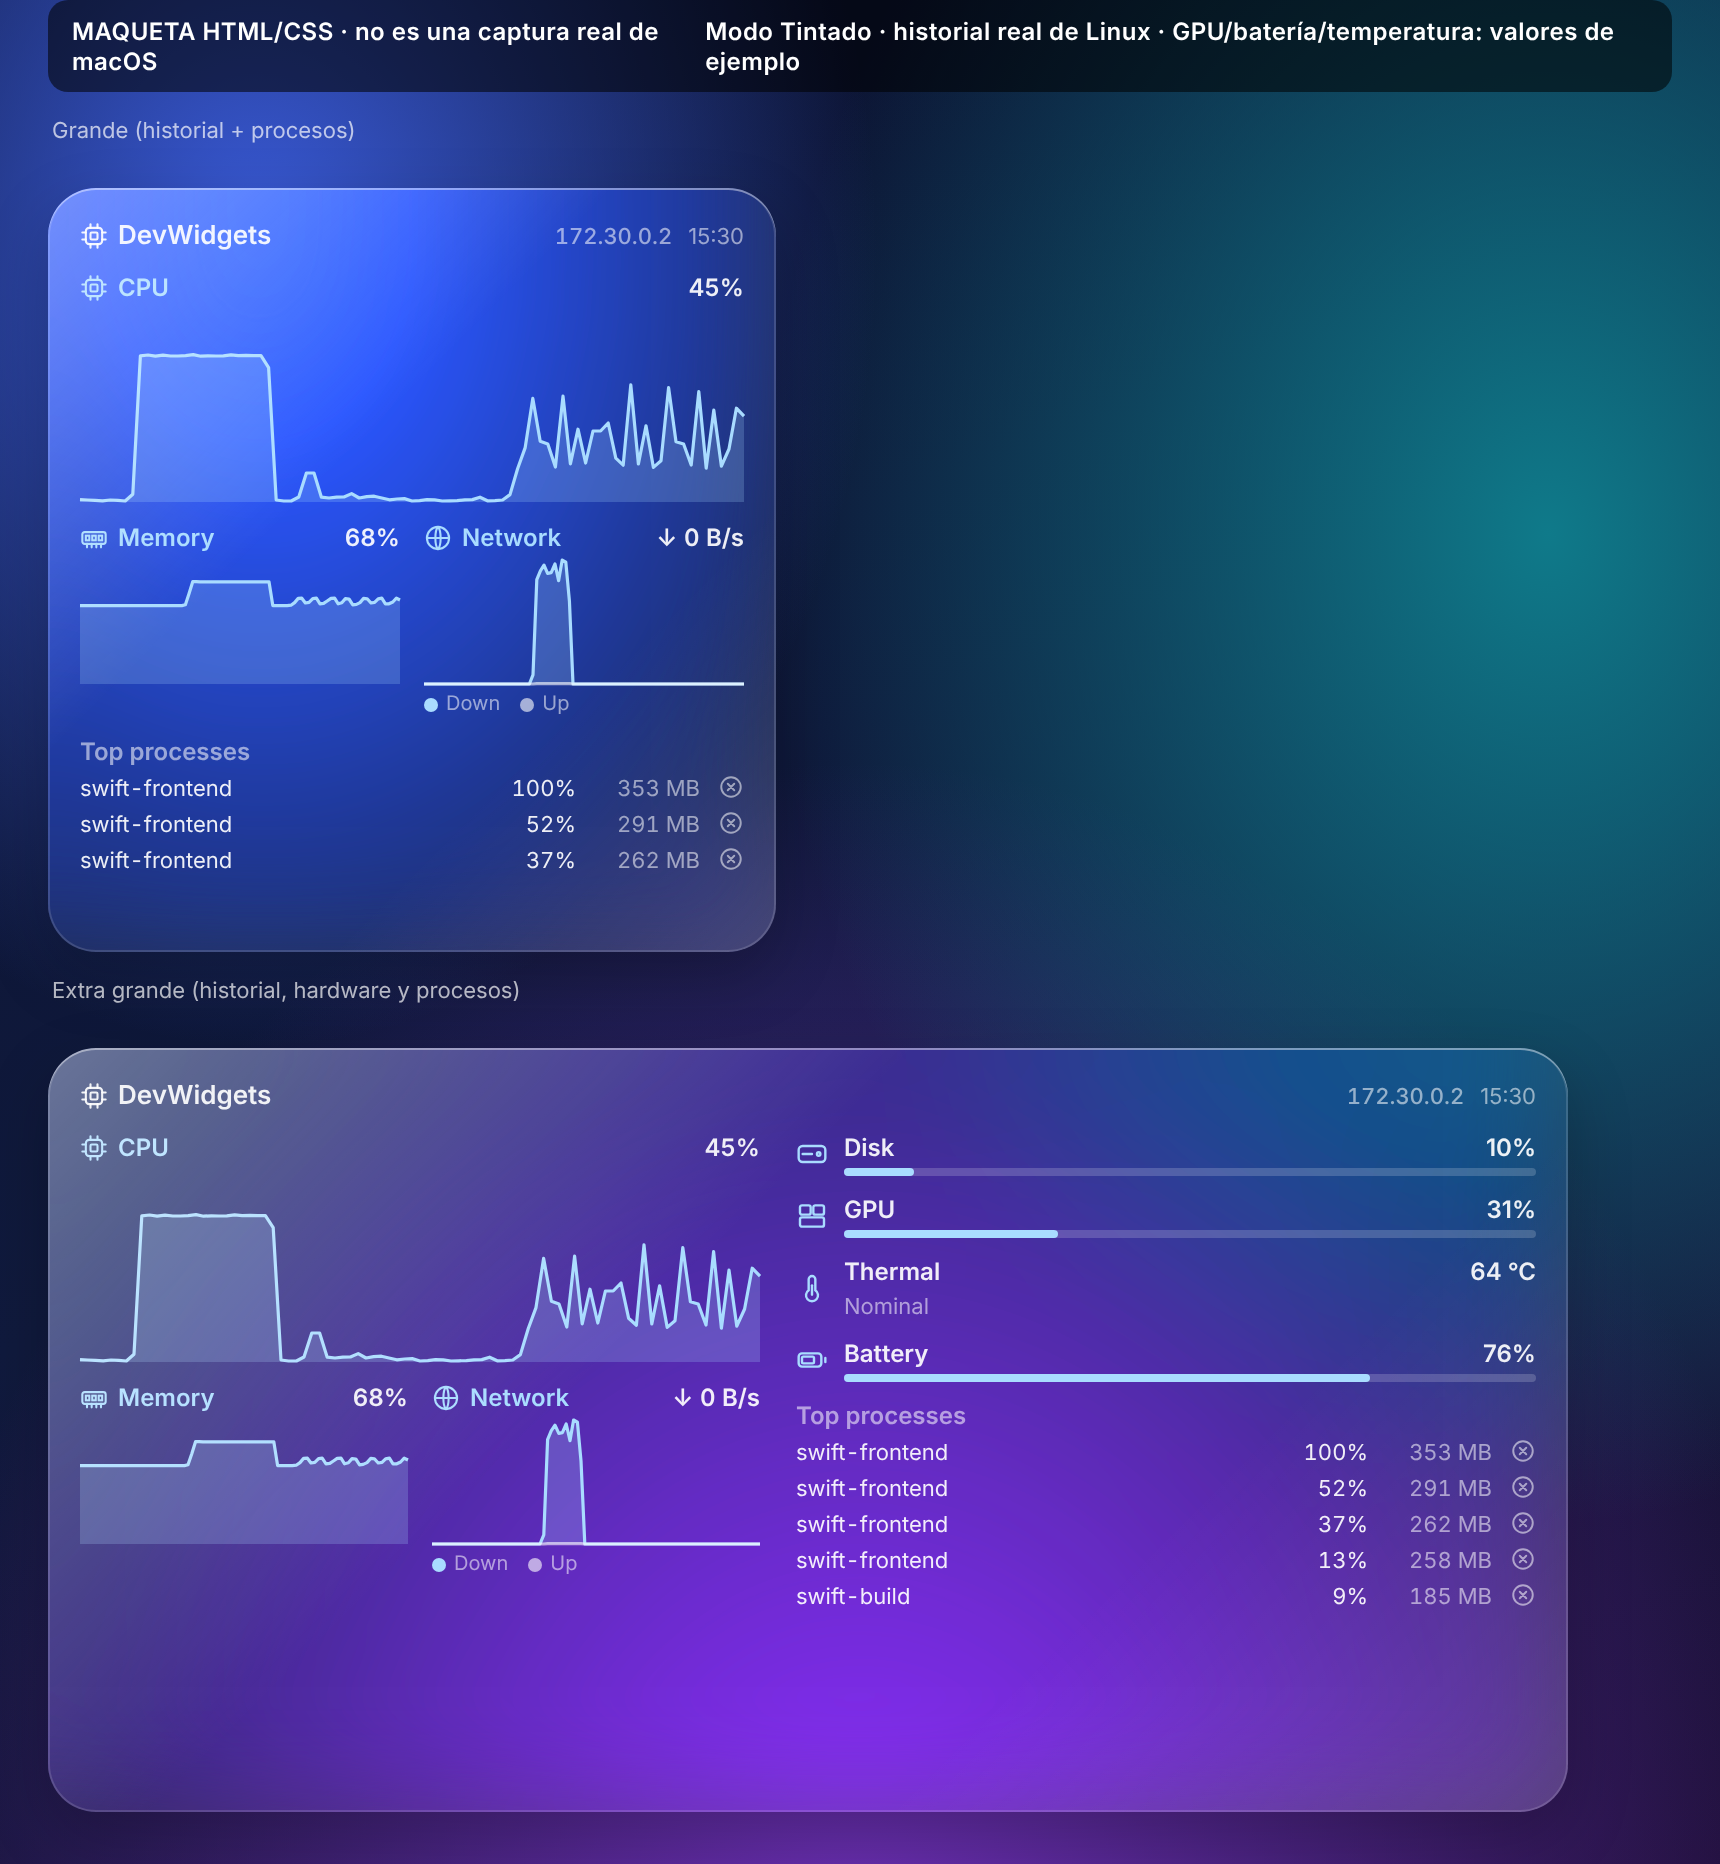
\includegraphics[width=0.9\textwidth]{images/mockup-dashboards-tinted.png}
\caption{\maqueta{} · Nuevo en la fase 2 · Modo tintado: gráficas y
barras toman el color único del sistema.}
\end{figure}

\begin{figure}[H]
\centering
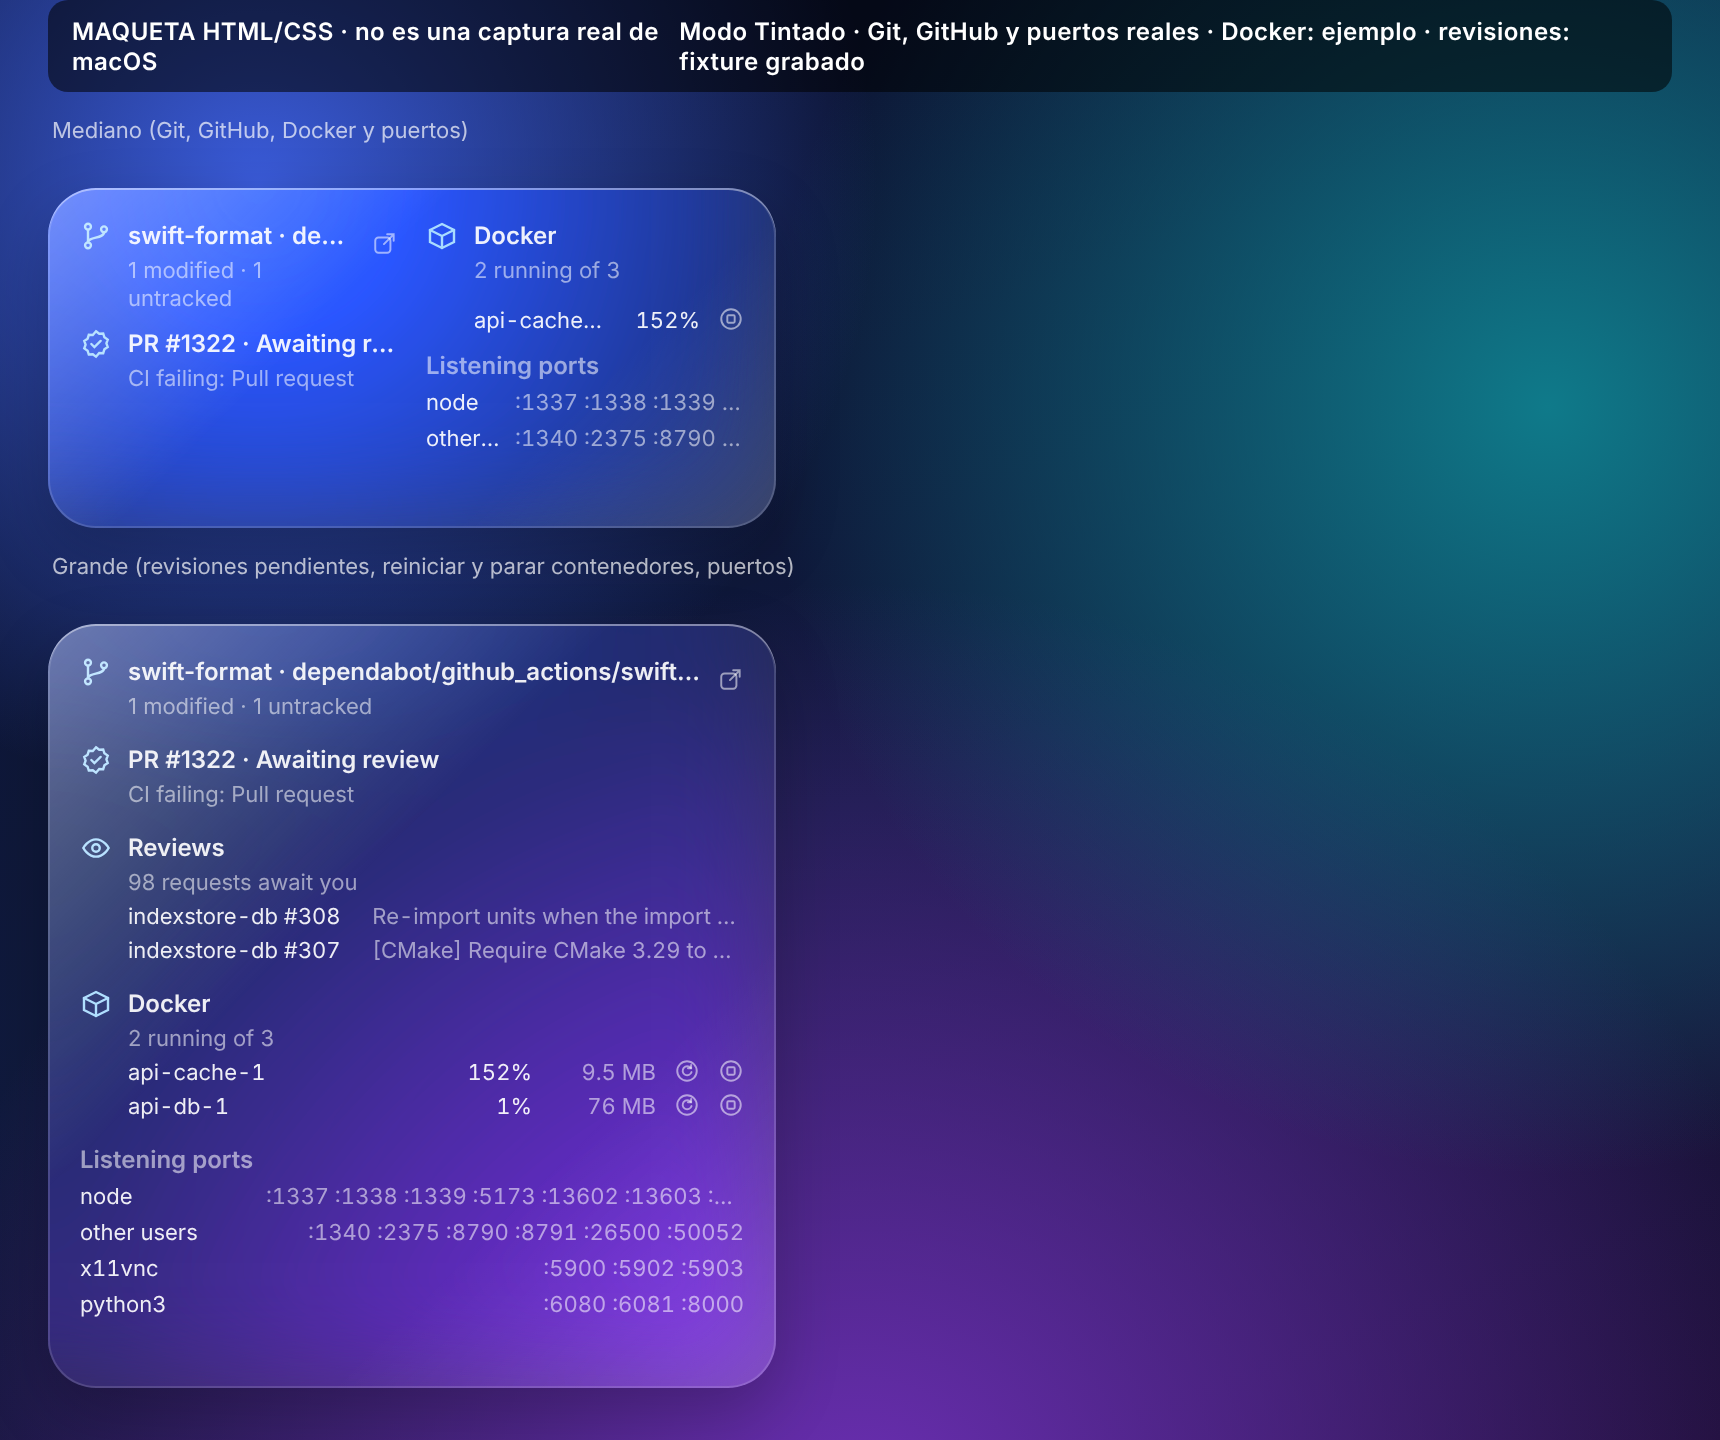
\includegraphics[width=0.9\textwidth]{images/mockup-context-tinted.png}
\caption{\maqueta{} · Nuevo en la fase 3 · Widget de contexto, modo
tintado.}
\end{figure}

\begin{figure}[H]
\centering
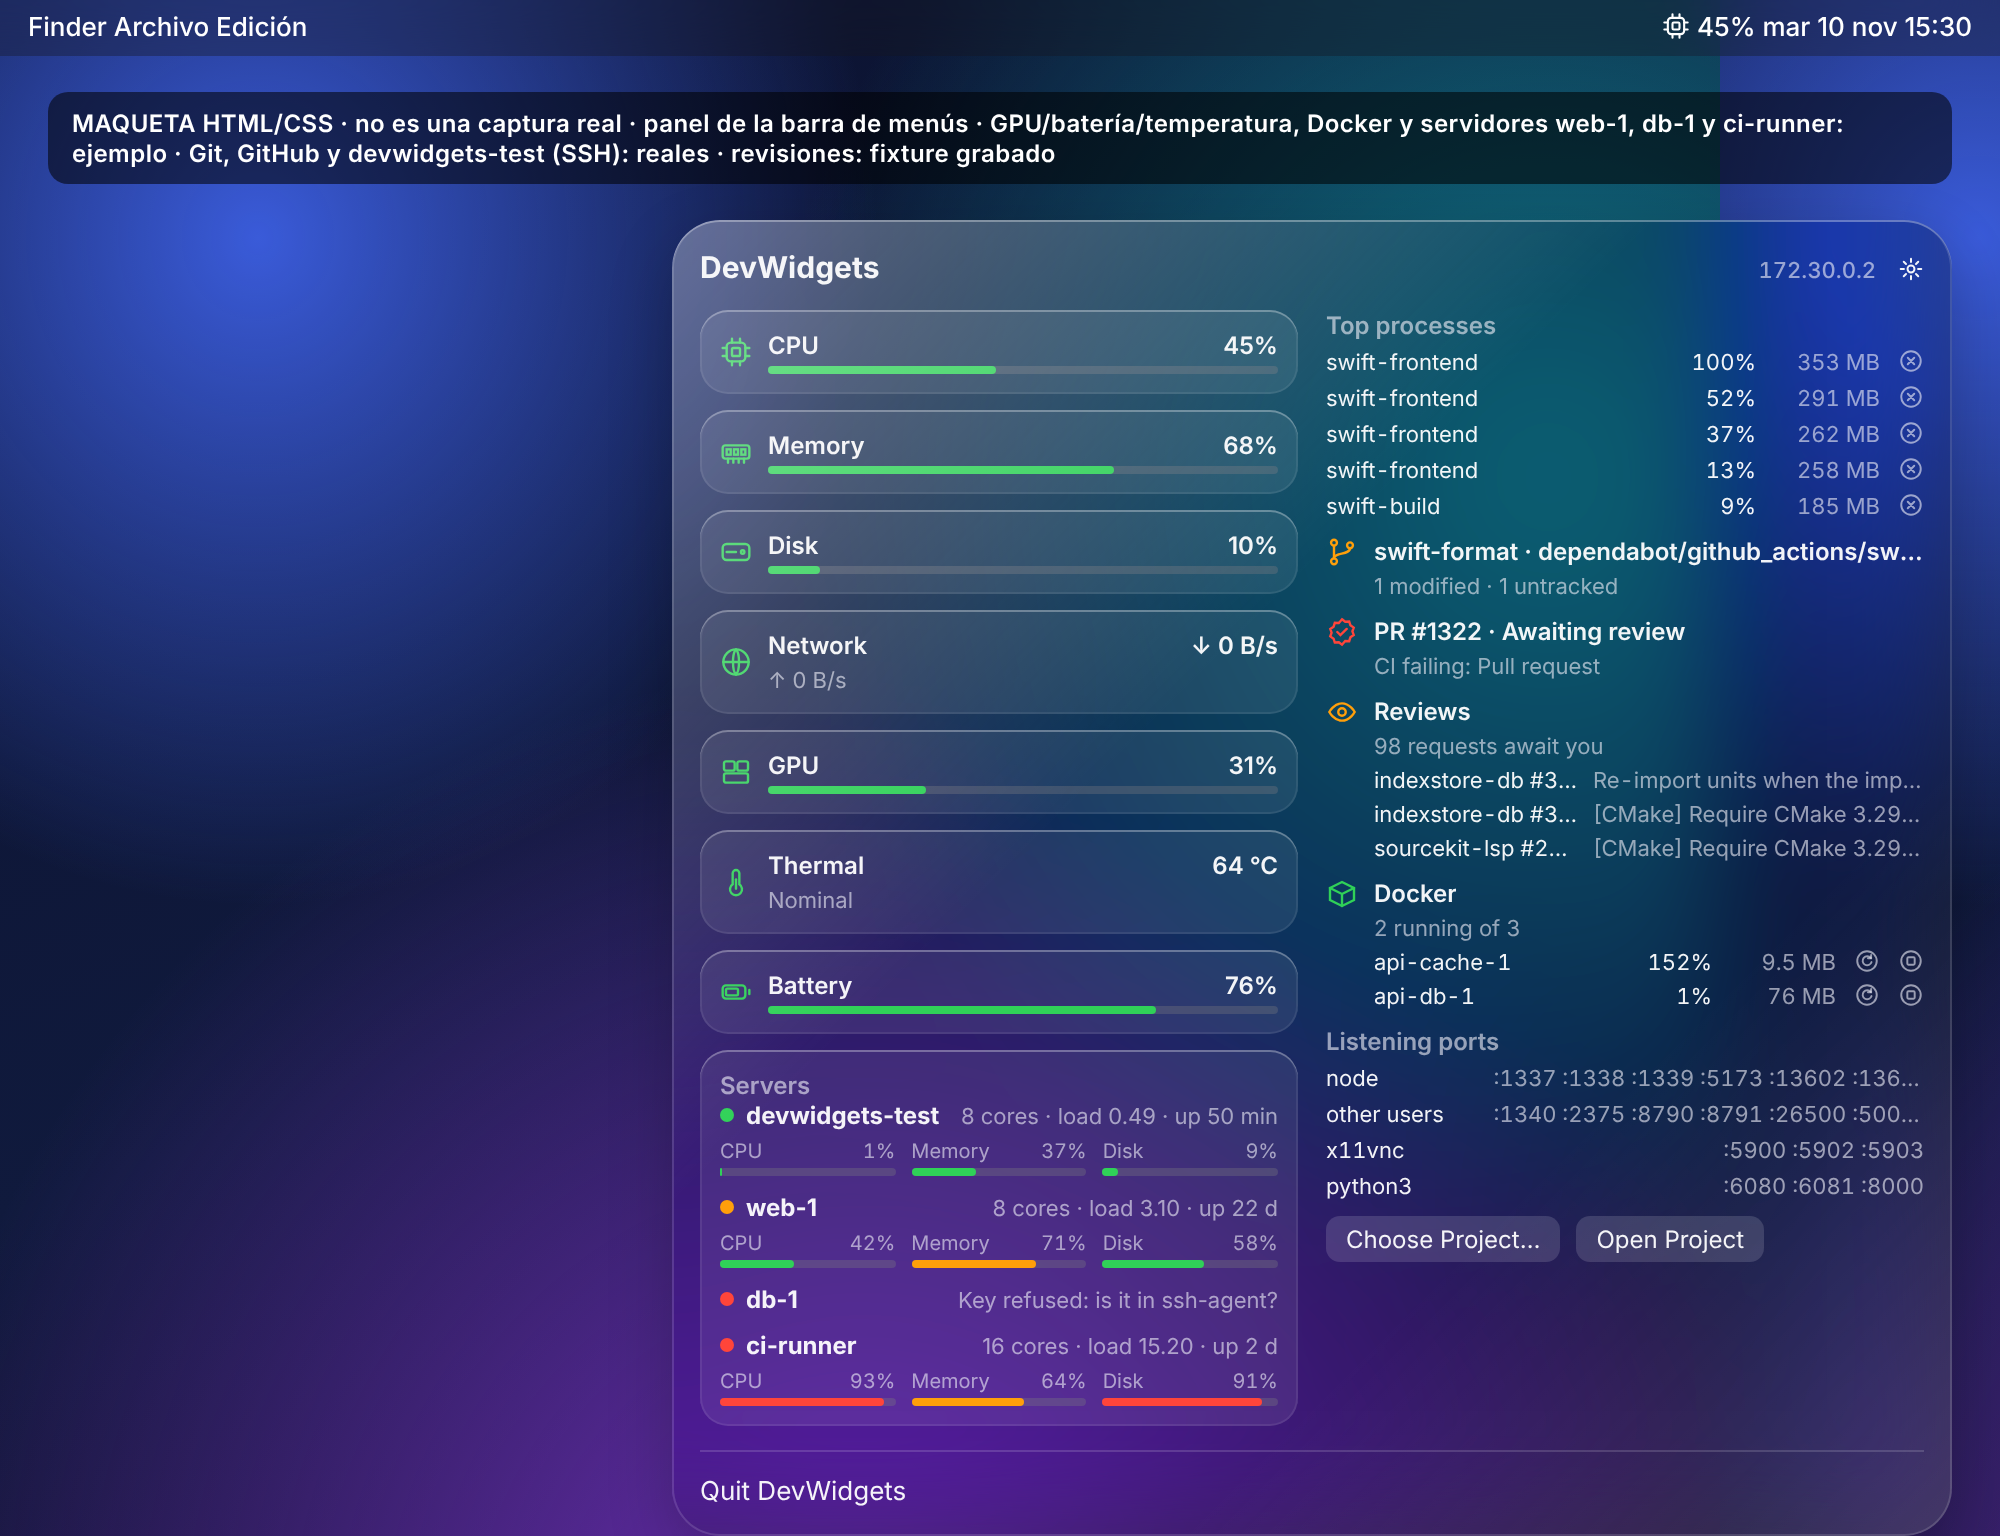
\includegraphics[width=\textwidth]{images/mockup-menubar-panel.png}
\caption{\maqueta{} · Actualizado en la fase 5 · Panel de la barra de
menús: métricas y servidores (fase 5) a la izquierda; revisiones
pendientes y reiniciar contenedor (fase 5); procesos con botón de cerrar, Git,
GitHub, Docker con botón de parar, puertos, ``Choose Project\ldots''
y ``Open Project'' a la derecha; engranaje de Ajustes. Git, GitHub,
puertos y \texttt{devwidgets-test} reales; revisiones grabadas; GPU,
temperatura, batería, Docker y los demás servidores: valores de
ejemplo.}
\end{figure}

\begin{figure}[H]
\centering
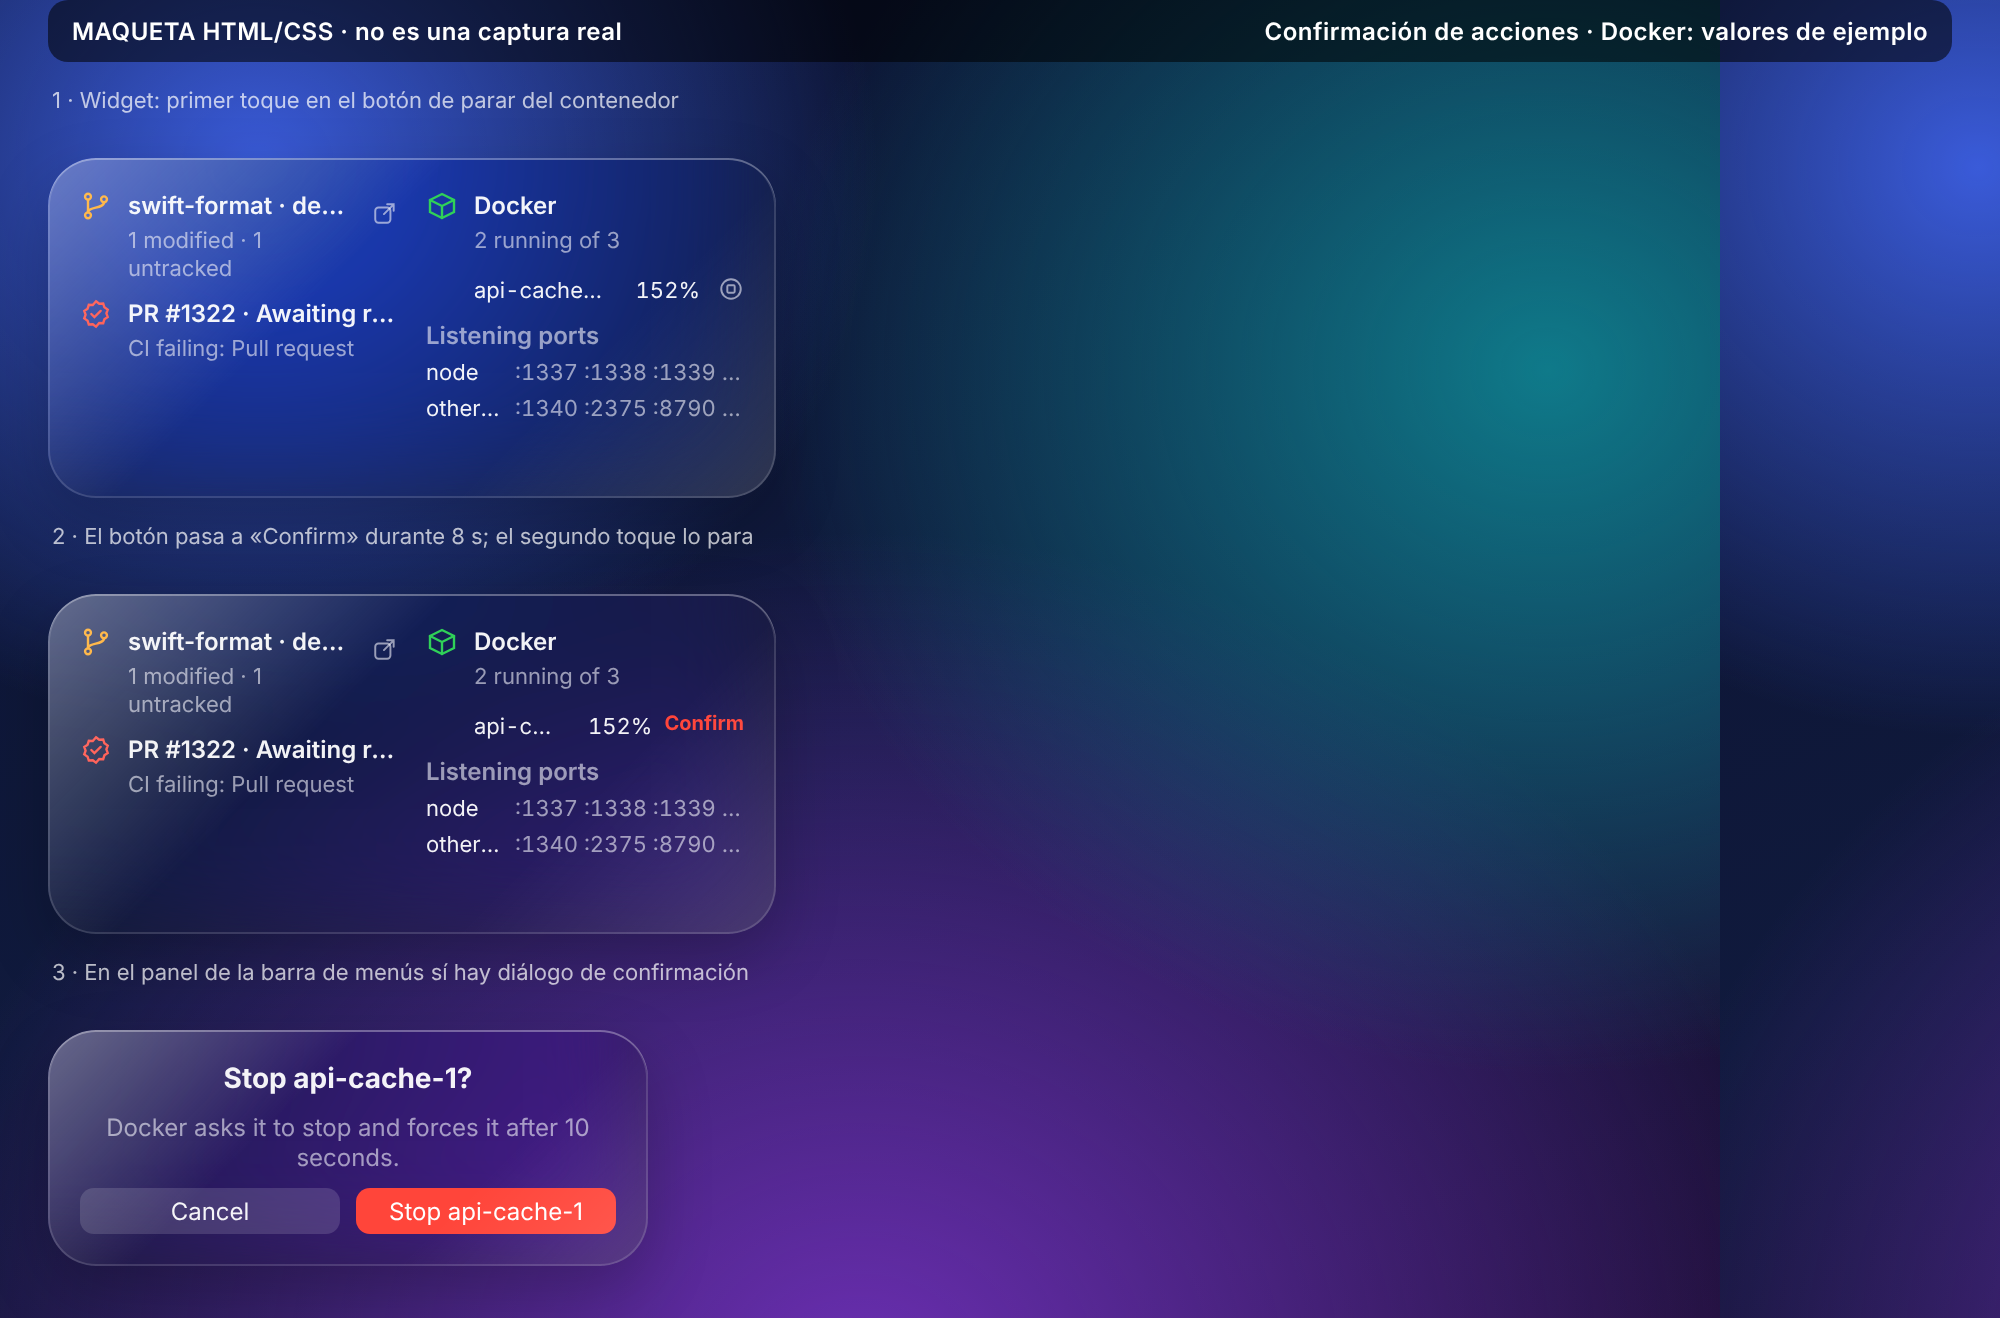
\includegraphics[width=0.9\textwidth]{images/mockup-actions-confirm.png}
\caption{\maqueta{} · Nuevo en la fase 4 · Confirmación de acciones:
en el widget, el primer toque arma la acción y el botón pasa a
``Confirm'' durante 8\,s; en el panel, diálogo del sistema. Docker:
valores de ejemplo.}
\end{figure}

\begin{figure}[H]
\centering
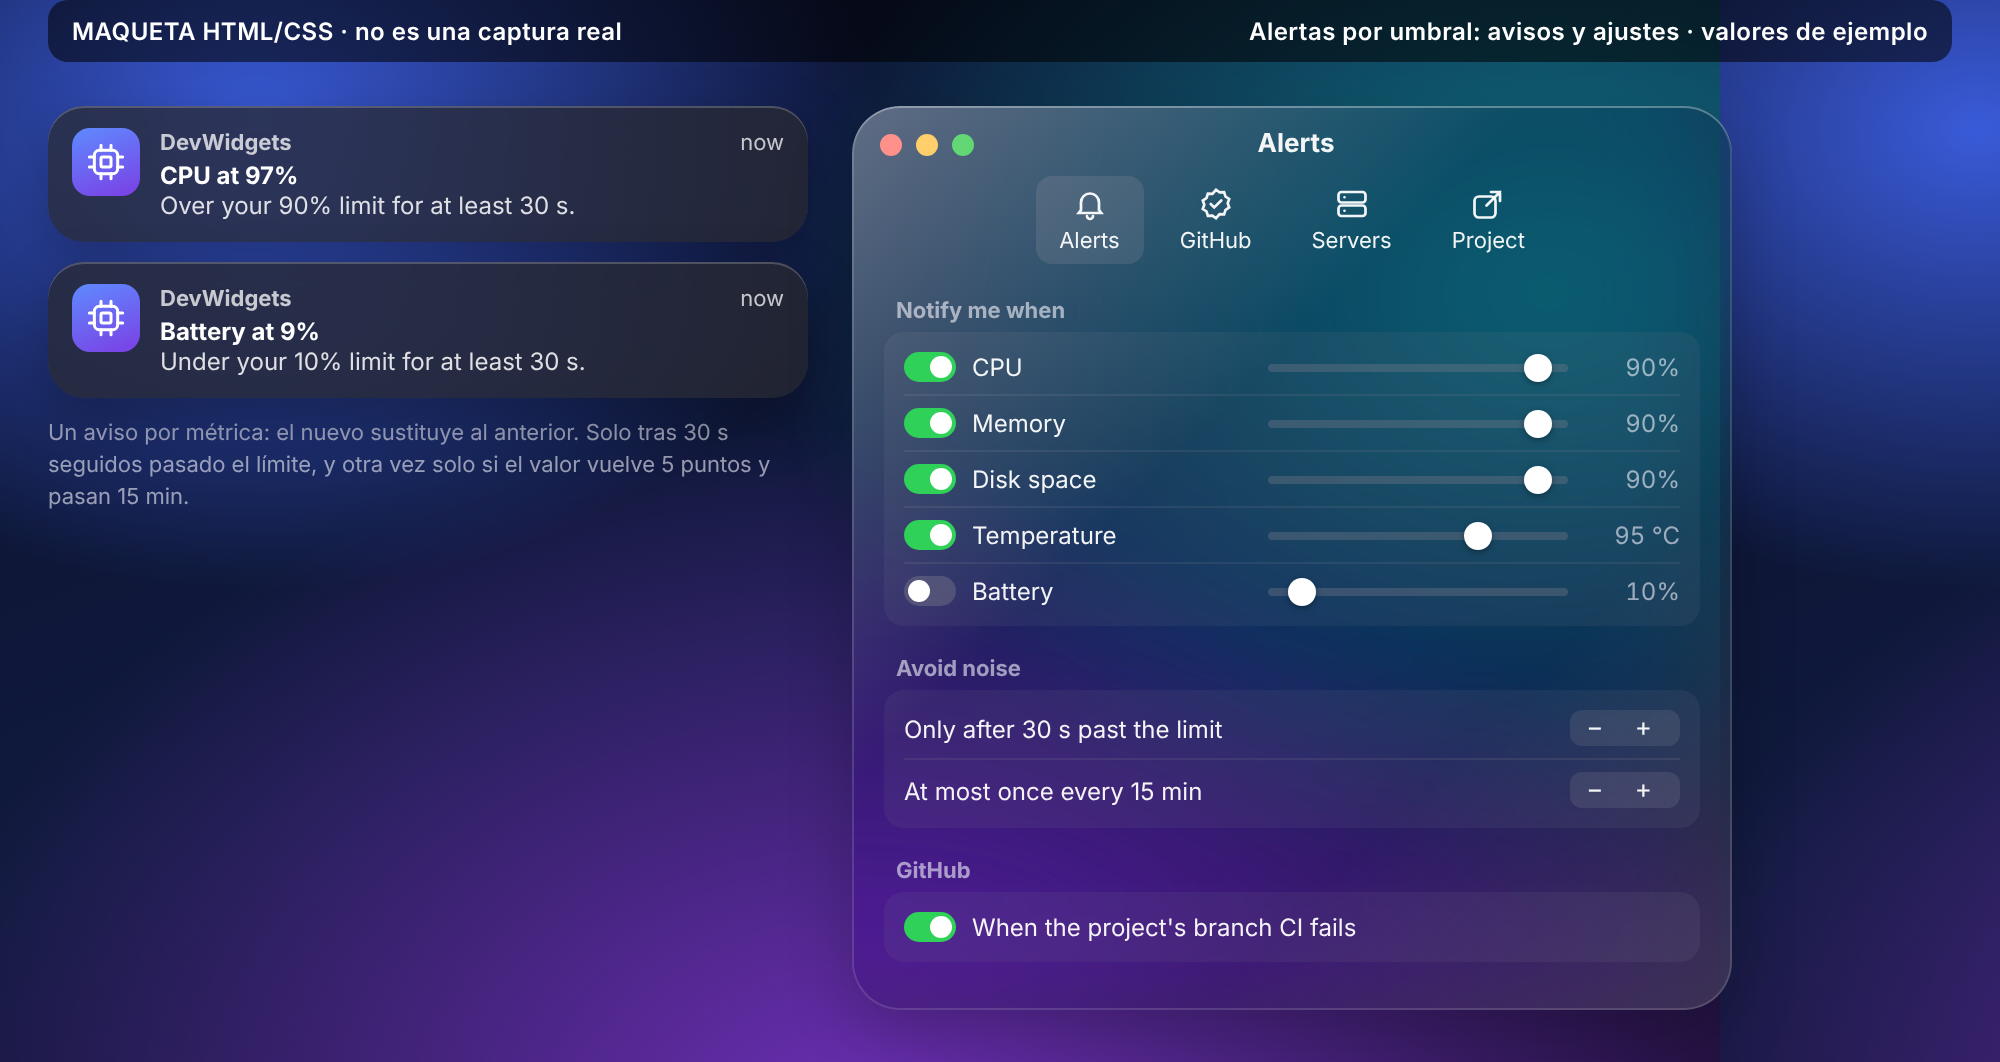
\includegraphics[width=\textwidth]{images/mockup-alerts.png}
\caption{\maqueta{} · Nuevo en la fase 4 · Alertas: dos avisos de
ejemplo y la pestaña de Ajustes con los umbrales y el antirruido.
Desde la fase 5, interruptor del aviso de CI fallido. Valores de
ejemplo.}
\end{figure}

\begin{figure}[H]
\centering
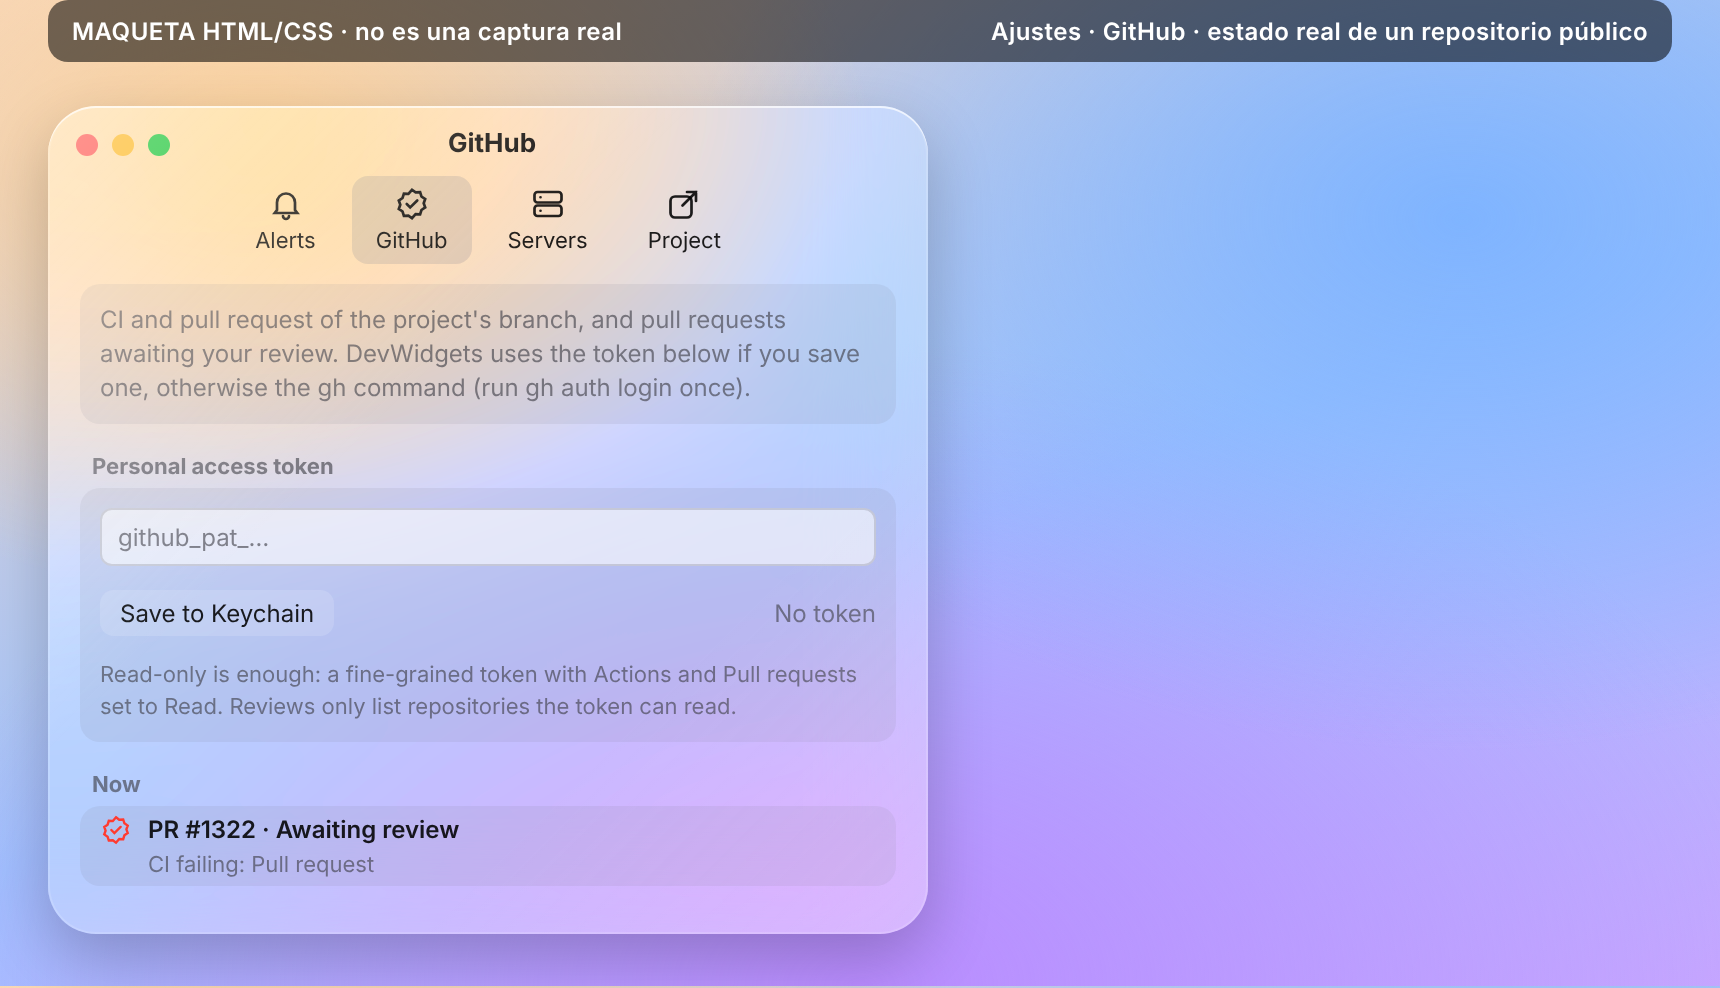
\includegraphics[width=0.75\textwidth]{images/mockup-settings-github.png}
\caption{\maqueta{} · Actualizado en la fase 5 · Ajustes de GitHub:
token en el Llavero (o \texttt{gh}) y estado actual; nueva pestaña
Servers. Estado real de un repositorio público.}
\end{figure}

\begin{figure}[H]
\centering
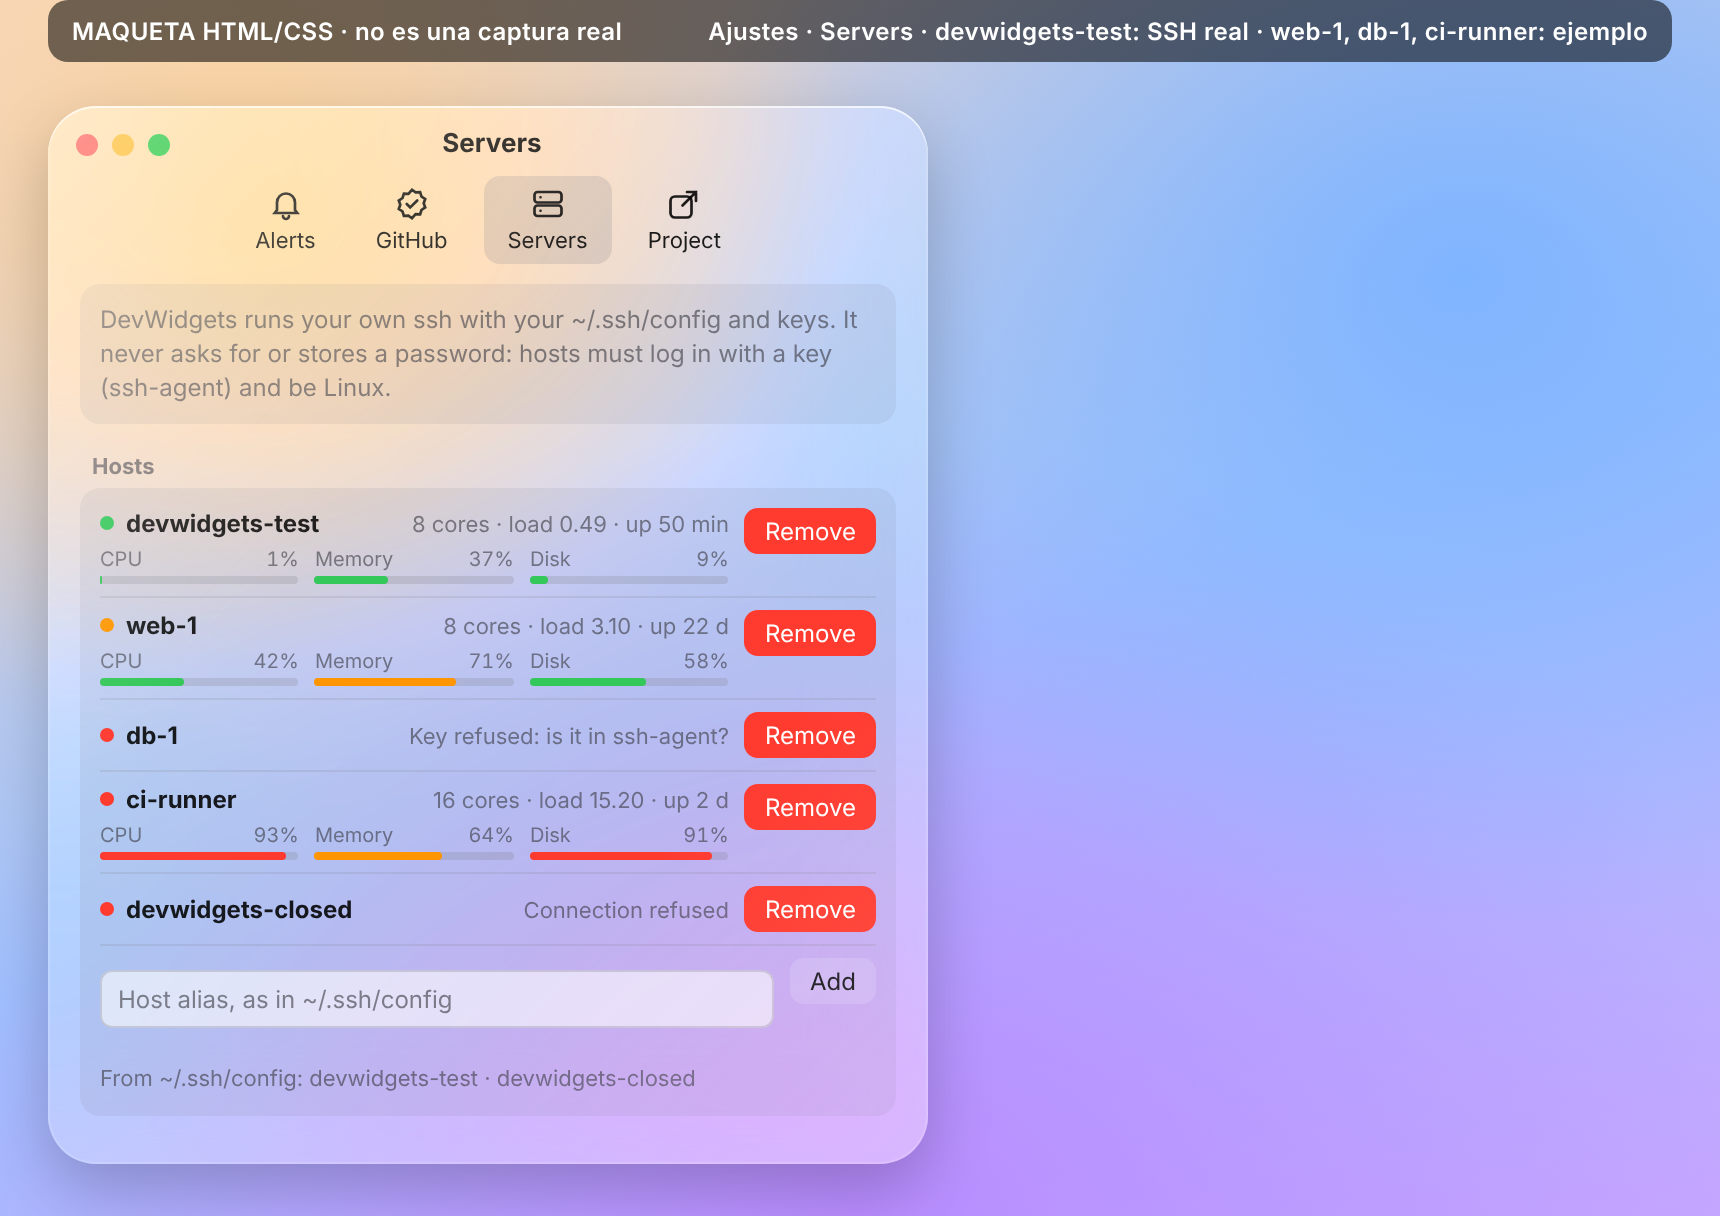
\includegraphics[width=0.75\textwidth]{images/mockup-settings-servers.png}
\caption{\maqueta{} · Nuevo en la fase 5 · Ajustes, pestaña Servers:
alias de \texttt{\textasciitilde/.ssh/config}, estado de cada uno y
sugerencias. \texttt{devwidgets-test} y \texttt{devwidgets-closed}
reales; el resto, ejemplo.}
\end{figure}

\begin{figure}[H]
\centering
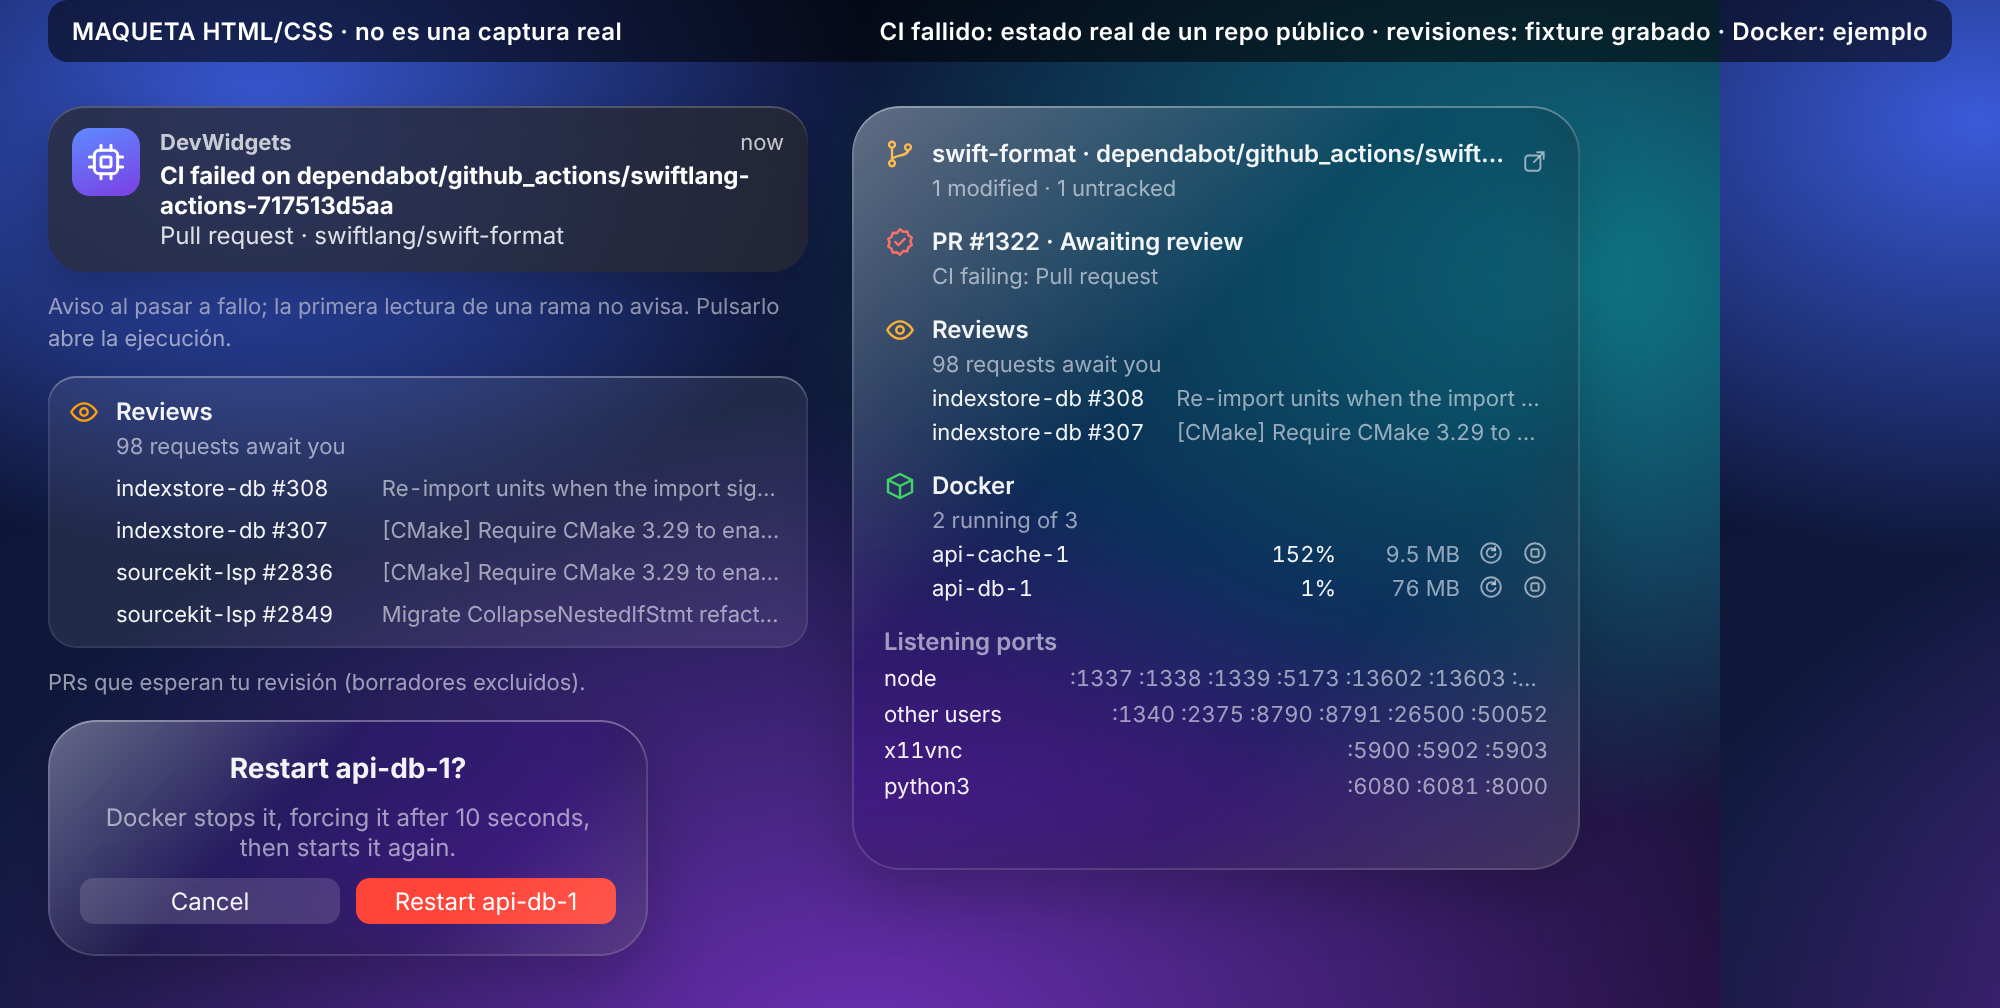
\includegraphics[width=\textwidth]{images/mockup-reviews-ci.png}
\caption{\maqueta{} · Nuevo en la fase 5 · Aviso de CI fallido (estado
real de \texttt{swift-format}), lista de pull requests pendientes de
revisión (búsqueda grabada con un revisor explícito), diálogo de
reiniciar y widget de contexto grande con revisiones y botones de
reiniciar y parar. Docker: ejemplo.}
\end{figure}

\section{Limitaciones conocidas}
\begin{itemize}
  \item \textbf{Temperatura en macOS}: solo estado térmico, sin
    grados (no hay API pública; leer el SMC sería frágil y privado).
  \item \textbf{GPU en Linux}: solo AMD (\texttt{gpu\_busy\_percent}).
    NVIDIA necesita NVML y llegará con la versión de Linux.
  \item \textbf{Procesos en macOS}: sin privilegios solo se ven los
    del usuario; los del sistema (\texttt{kernel\_task},
    \texttt{WindowServer}) no aparecen.
  \item \textbf{Disco en macOS}: se suman todos los
    \texttt{IOBlockStorageDriver}, también discos externos e imágenes
    montadas.
  \item \textbf{Histórico}: 5 minutos a 1 muestra/s, guardado en el
    snapshot. Los widgets lo ven cada vez que WidgetKit los recarga
    (unos 60\,s), no en continuo.
  \item \textbf{Puertos}: solo TCP en escucha. Sin privilegios, los
    de otros usuarios aparecen como ``other users'' (en Linux) o no
    aparecen (en macOS, \texttt{lsof}).
  \item \textbf{Docker}: un contexto remoto lento puede agotar los 5\,s
    y mostrarse como ``Not running''. La CPU de un contenedor es la
    que da \texttt{docker stats} (100\,\% = un núcleo).
  \item \textbf{Git}: un solo proyecto; en repositorios enormes
    \texttt{git status} puede tardar. Los submódulos cuentan como
    cambios del repositorio principal.
  \item \textbf{Contexto en widgets}: mejorado en la fase 4 (recarga
    al cambiar, como mucho cada 30\,s), pero WidgetKit puede retrasar
    las recargas. La CPU de los contenedores en el widget puede estar
    desfasada, porque no provoca recargas.
  \item \textbf{GitHub}: la búsqueda de revisiones no admite ETags
    (se consulta cada 5\,min); como mucho 10 pull requests. Solo
    \texttt{github.com}, no GitHub Enterprise. La consulta anónima
    solo existe en la sonda.
  \item \textbf{Servidores}: solo Linux; un disco por servidor; sin
    procesos ni contenedores remotos. Las sugerencias siguen
    \texttt{Include}, pero no evalúan bloques \texttt{Match}. Un
    servidor que pide contraseña o 2FA aparece como clave rechazada
    (y no como ``caído'').
  \item \textbf{Linux, bandeja}: GNOME no tiene bandeja sin la
    extensión AppIndicator; sin ella, la app es una ventana normal
    (cerrarla la cierra). El icono no tiene menú contextual: un clic
    muestra u oculta el panel.
  \item \textbf{Linux, aspecto}: GTK no tiene desenfoque del fondo de
    la ventana; el ``cristal'' es translucidez, bordes y sombras. Sin
    GPU, las animaciones gastan más CPU.
  \item \textbf{Linux, empaquetado}: solo \texttt{.deb} para
    \texttt{amd64}; Flatpak sin construir y con acceso limitado al
    sistema; ni RPM ni arm64.
  \item \textbf{Sockets de \texttt{ControlMaster}} en \texttt{/tmp}
    (rutas cortas: el límite de un socket Unix es de 104 bytes); si la
    carpeta no es privada, se conecta sin compartir.
  \item \textbf{Acciones}: cerrar un proceso solo envía SIGTERM y
    solo funciona con procesos del usuario; un fallo de permisos se
    muestra como rechazo.
  \item Espacio de disco con \texttt{statvfs}: en APFS no incluye el
    espacio purgable.
  \item WidgetKit puede ignorar parte de las recargas pedidas.
  \item La lógica de presentación de las maquetas de macOS sigue
    duplicada en JavaScript hasta que haya capturas reales.
\end{itemize}

\section{Estado general y lo que falta}\label{sec:estado}
\paragraph{Estado.} El núcleo (métricas, contexto, GitHub,
servidores, alertas y acciones) está completo y probado en Linux. La
app de Linux funciona y se instala con un \texttt{.deb}. La app y los
widgets de macOS compilan con Xcode y la app arranca; falta firmarlos
con tu equipo y verlos en el escritorio. Ninguna parte se ha publicado.

\paragraph{Necesita un Mac (o el runner \texttt{macos-26}).}
\begin{itemize}
  \item[$\checkmark$] Compilar \texttt{DevWidgetsDarwin}, la sonda y
    las pruebas con SwiftPM en un Mac real (sección~\ref{sec:mac}).
  \item[$\checkmark$] Comprobar los tipos de la app, los widgets y los
    App Intents (sin errores tras 6 correcciones).
  \item[$\checkmark$] Generar el proyecto con XcodeGen y compilar la
    \texttt{.app}, la extensión y los App Intents con
    \texttt{xcodebuild} (sección~\ref{sec:xcodebuild}).
  \item[$\checkmark$] Cristal del sistema y diseño más denso
    (sección~\ref{sec:cristal}).
  \item[$\checkmark$] Imágenes reales de los widgets con
    \texttt{ImageRenderer}, claro y oscuro, en todos los tamaños.
  \item[$\square$] Capturas del escritorio real (Liquid Glass, modo
    tintado) y de las ventanas de la app.
  \item[$\checkmark$] Firmar con tu equipo; App Group con prefijo de
    equipo, sin registros (sección~\ref{sec:appgroup}).
  \item[$\square$] Añadir los widgets al escritorio y probar el doble
    toque.
  \item[$\square$] Distribuir: Developer ID, notarización y DMG
    (sección~\ref{sec:distribucion}; requiere la cuenta de pago).
  \item[$\checkmark$] Valores reales de GPU (clave), disco, memoria,
    batería y estado térmico en reposo (sección~\ref{sec:mac}).
  \item[$\square$] GPU bajo carga, número exacto de procesos visibles
    y estado térmico con calor.
  \item[$\square$] Llavero (token), notificaciones, \texttt{ssh} con
    el agente de macOS, \texttt{lsof}, abrir el proyecto.
\end{itemize}

\paragraph{Necesita publicar el repositorio (tu decisión).}
\begin{itemize}
  \item[$\square$] Subirlo a GitHub (puede ser privado) para que el
    flujo \texttt{ci.yml} compile en \texttt{macos-26} y en Linux.
  \item[$\square$] Página web en los metadatos (quita el único aviso
    de \texttt{lintian} y AppStream) y, si quieres, publicar el
    \texttt{.deb} como \emph{release}.
  \item[$\square$] Elegir licencia (hoy ``todos los derechos
    reservados'' en \texttt{copyright}).
\end{itemize}

\paragraph{Se puede hacer sin Mac ni publicar.}
\begin{itemize}
  \item[$\square$] Construir y probar el Flatpak con
    \texttt{flatpak-spawn --host}.
  \item[$\square$] Probar en GNOME, KDE y Wayland reales.
  \item[$\square$] GitHub con sesión y Docker real.
  \item[$\square$] Menú en el icono de la bandeja; GPU NVIDIA.
\end{itemize}

\section{Registro de cambios}
\subsection*{Fase 6, adenda 3 · App Group para cualquier usuario · 10 de noviembre de 2026}
\begin{itemize}
  \item App Group con prefijo del equipo, leído del
    \texttt{Info.plist}; equipo solo en \texttt{project.yml}.
  \item El panel avisa si los widgets no reciben datos; el widget
    vacío ya no dice que la app está cerrada.
  \item Sección de distribución en el README y en el informe.
\end{itemize}

\subsection*{Fase 6, adenda 2 · Xcode y cristal nativo · 10 de noviembre de 2026}
\begin{itemize}
  \item XcodeGen y \texttt{xcodebuild} con Xcode 27.2: app, extensión
    y App Intents compilan sin errores ni avisos; app firmada \emph{ad
    hoc} en marcha y extensión registrada. La firma real necesita un
    equipo (App Group).
  \item Cristal: sin fondo propio (\texttt{containerBackground} del
    sistema), color solo para avisos, gráficas según
    \texttt{widgetRenderingMode}, tipografía como los widgets de Apple.
  \item Espacio: pequeño al estilo del widget de batería, filas que
    llenan el mediano, más filas en contexto, servidores y procesos.
  \item Imágenes en cristal, oscuro y claro;
    \texttt{tools/compose\_widget\_renders.py} y
    \texttt{tools/compose\_comparison.py} (solo los widgets, sobre
    fondo transparente, sin fondo de pantalla ni capturas del
    escritorio).
\end{itemize}

\subsection*{Fase 6, adenda · Primera compilación en Mac · 10 de noviembre de 2026}
\begin{itemize}
  \item Corregidos los errores de compilación de
    \texttt{DevWidgetsDarwin} y el aviso de \texttt{readSysctl}.
  \item La sonda usa el lector de macOS en macOS; prueba de cerrar
    procesos portable; suite \texttt{DarwinReaderTests}.
  \item \texttt{tools/swift\_test\_clt.sh} para probar con solo las
    Command Line Tools; sin avisos de ficheros sin declarar.
  \item \texttt{swift build} y \texttt{swift test} (235 pruebas) en verde
    en un Mac real; lecturas reales comparadas
    (sección~\ref{sec:mac}).
  \item \texttt{tools/check\_macos\_clt.sh}: comprobación de tipos de
    la app y los widgets; 6 errores corregidos (concurrencia,
    \texttt{MetricHeader}, \texttt{AppEnum} público, gráficas vacías
    en las vistas previas, alineación del widget pequeño, barras de
    servidores).
  \item \texttt{macOS/Render} y \texttt{tools/render\_widgets\_clt.sh}:
    imágenes reales de los widgets, que sustituyen a sus maquetas;
    \texttt{LayoutFamily} para elegir el tamaño fuera de WidgetKit.
\end{itemize}

\subsection*{Fase 6 · 10 de noviembre de 2026}
\begin{itemize}
  \item App de Linux (\texttt{devwidgets-linux}) con GTK~4 y
    libadwaita por C directo: panel con tamaños de macOS, aspecto de
    cristal, claro y oscuro, bandeja StatusNotifierItem,
    notificaciones, ajustes, acciones con confirmación.
  \item \texttt{DevWidgetsLinuxShell} (lógica sin GTK, con pruebas).
  \item Núcleo: \texttt{SSHConfigReader} con \texttt{Include}, disco
    remoto elegible, \texttt{ServerDownMonitor},
    \texttt{DeveloperContextRefresher}. 232 pruebas.
  \item macOS (sin compilar): aviso de servidor caído, disco por
    servidor, sugerencias con \texttt{Include}, código común movido al
    núcleo.
  \item Paquete \texttt{.deb} (\texttt{tools/package\_deb.sh}),
    \texttt{.desktop}, AppStream, icono, página de manual; manifiesto
    Flatpak experimental.
  \item Correcciones de fases anteriores
    (sección~\ref{sec:correcciones6}).
  \item Capturas reales de Linux e informe v6.
\end{itemize}

\subsection*{Fase 5 · 10 de noviembre de 2026}
\begin{itemize}
  \item Núcleo: servidores por SSH (\texttt{RemoteHost},
    \texttt{RemoteProbe}, \texttt{SSHReader}, \texttt{RemoteTracker}),
    caché de ETags (\texttt{GitHubClient}), revisiones pendientes,
    \texttt{CIFailureMonitor}, \texttt{ContainerController} con
    reiniciar, \texttt{BlockingWork}, \texttt{ReloadThrottle}. 198
    pruebas.
  \item macOS (sin compilar): widget de servidores, sección de
    servidores en el panel, pestaña de Ajustes, revisiones en panel y
    widget, aviso de CI que abre la ejecución, botón de reiniciar.
  \item \texttt{devwidgets-probe servers} y \texttt{reviews};
    \texttt{tools/ssh\_test\_server.sh}.
  \item Correcciones de fases anteriores
    (sección~\ref{sec:correcciones5}).
  \item Maquetas nuevas e informe v5.
\end{itemize}

\subsection*{Fase 4 · 10 de noviembre de 2026}
\begin{itemize}
  \item Núcleo: GitHub (remotos, pull request, CI, revisiones,
    transportes REST y \texttt{gh}, calendario con límite de
    peticiones), alertas con antirruido, acciones (bandeja,
    confirmación, cerrar proceso, parar contenedor),
    \texttt{ContextChangeTracker}. 151 pruebas.
  \item macOS (sin compilar): App Intents de los widgets, token en el
    Llavero, notificaciones, ventana de Ajustes, abrir proyecto,
    botones en panel y widgets.
  \item Objetivo \texttt{DevWidgetsPresentation} compilado en Linux.
  \item \texttt{devwidgets-probe github}.
  \item Correcciones de fases anteriores
    (sección~\ref{sec:correcciones4}).
  \item Maquetas nuevas e informe v4.
\end{itemize}

\subsection*{Fase 3 · 10 de noviembre de 2026}
\begin{itemize}
  \item Núcleo: \texttt{CommandRunner} con límite de tiempo, Docker
    (\texttt{ps}/\texttt{stats}), puertos (\texttt{/proc/net} y
    \texttt{lsof}), Git (\texttt{porcelain=v2}),
    \texttt{DeveloperContext}, \texttt{JSONFileStore}. 102 pruebas.
  \item macOS (sin compilar): \texttt{DeveloperContextModel} cada
    10\,s, selector de proyecto, widget de contexto mediano y grande,
    panel en dos columnas.
  \item \texttt{devwidgets-probe context}.
  \item Correcciones de fases anteriores
    (sección~\ref{sec:correcciones3}).
  \item Maquetas nuevas e informe v3.
\end{itemize}

\subsection*{Fase 2 · 10 de noviembre de 2026}
\begin{itemize}
  \item Núcleo: GPU, temperatura, batería, ranking de procesos, IP
    local, histórico de red, interfaces físicas, lectores de
    \texttt{/sys} y \texttt{/proc/[pid]/stat}. 74 pruebas.
  \item macOS (sin compilar): red de 64 bits, E/S de disco y GPU por
    IOKit, batería, estado térmico y procesos con \texttt{libproc}.
  \item Widgets grande y extra grande con Swift Charts; métricas
    nuevas en el widget configurable y en la barra de menús.
  \item Correcciones de la fase 1 (sección~\ref{sec:correcciones}).
  \item Maquetas nuevas, plan del runner de macOS e informe v2.
\end{itemize}

\subsection*{Fase 1 · 10 de noviembre de 2026}
\begin{itemize}
  \item Repositorio, plan por fases, README y CI preparado.
  \item Herramientas de calidad: swift-format, SwiftLint y
    \texttt{check\_style.py} con autotest; \texttt{tools/lint.sh}.
  \item \texttt{DevWidgetsCore}: CPU, RAM/swap/presión, disco,
    red, niveles de carga, histórico, snapshots, lectores de
    \texttt{/proc}. 51 pruebas.
  \item \texttt{DevWidgetsDarwin}: lector de macOS (sin compilar).
  \item App de barra de menús y widgets pequeño y mediano con
    métrica elegible (sin compilar).
  \item Maquetas en modo claro, oscuro y tintado, e informe v1.
\end{itemize}
\end{document}
